\documentclass[conference]{IEEEtran}
\IEEEoverridecommandlockouts
\usepackage{cite}
\usepackage{amsmath,amssymb,amsfonts}
\usepackage{graphicx}
\usepackage{textcomp}
\usepackage{xcolor}
\usepackage{booktabs}
\usepackage{array}
\usepackage{multirow}
\usepackage{balance}
\usepackage[hidelinks]{hyperref}

% Protocol v1 numbers, generated from results/v1 by scripts/a4_protocol_v1.py --tables.
% Allen atlas numbers, generated from results/large_scale by scripts/large_scale/make_tables.py.
% \V{key} prints one value. An unknown key prints ??key in bold and warns, so nothing goes stale silently.
\makeatletter
\newcommand{\V}[1]{\ifcsname v@#1\endcsname\csname v@#1\endcsname\else\textbf{??\detokenize{#1}}\PackageWarning{numbers}{undefined value #1}\fi}
\makeatother
% Generated by scripts/a4_protocol_v1.py from results/v1. Do not edit by hand.
% seeds 3 to 9 confirmatory, PBMC14K seeds [0, 1, 2, 3, 4]
\expandafter\def\csname v@A3.C2.leiden\endcsname{0.118}
\expandafter\def\csname v@A3.C2.mica\endcsname{0.197}
\expandafter\def\csname v@A3.C3.five.leiden\endcsname{0.177}
\expandafter\def\csname v@A3.C3.five.mica\endcsname{0.534}
\expandafter\def\csname v@A3.C3.four.mica\endcsname{0.231}
\expandafter\def\csname v@A3.C5.leiden\endcsname{0.635}
\expandafter\def\csname v@A3.C5.mica\endcsname{0.473}
\expandafter\def\csname v@A3.F.leiden\endcsname{0.543}
\expandafter\def\csname v@A3.F.mica\endcsname{0.662}
\expandafter\def\csname v@A3.M.leiden\endcsname{0.452}
\expandafter\def\csname v@A3.M.mica\endcsname{0.473}
\expandafter\def\csname v@AMI.F.kmeans\endcsname{0.525}
\expandafter\def\csname v@AMI.F.leiden\endcsname{0.677}
\expandafter\def\csname v@AMI.F.mica\endcsname{0.771}
\expandafter\def\csname v@AMI.M.kmeans\endcsname{0.461}
\expandafter\def\csname v@AMI.M.leiden\endcsname{0.592}
\expandafter\def\csname v@AMI.M.mica\endcsname{0.575}
\expandafter\def\csname v@C1.F.gap.s02\endcsname{0.119}
\expandafter\def\csname v@C1.F.leads\endcsname{7 of 7}
\expandafter\def\csname v@C1.F.verdict\endcsname{holds}
\expandafter\def\csname v@C1.M.gap.s02\endcsname{0.020}
\expandafter\def\csname v@C1.M.leads\endcsname{3 of 7}
\expandafter\def\csname v@C1.M.verdict\endcsname{fails}
\expandafter\def\csname v@C2.kmeans\endcsname{0.079}
\expandafter\def\csname v@C2.leiden\endcsname{0.179}
\expandafter\def\csname v@C2.leiden.s02\endcsname{0.118}
\expandafter\def\csname v@C2.mica\endcsname{0.292}
\expandafter\def\csname v@C2.mica.s02\endcsname{0.198}
\expandafter\def\csname v@C2.verdict\endcsname{holds}
\expandafter\def\csname v@C3.five_smallest.kmeans.atone\endcsname{7}
\expandafter\def\csname v@C3.five_smallest.kmeans.share\endcsname{0.092}
\expandafter\def\csname v@C3.five_smallest.kmeans.span\endcsname{2.0}
\expandafter\def\csname v@C3.five_smallest.leiden.atone\endcsname{7}
\expandafter\def\csname v@C3.five_smallest.leiden.share\endcsname{0.142}
\expandafter\def\csname v@C3.five_smallest.leiden.span\endcsname{3.2}
\expandafter\def\csname v@C3.five_smallest.mica.atone\endcsname{45}
\expandafter\def\csname v@C3.five_smallest.mica.share\endcsname{0.493}
\expandafter\def\csname v@C3.five_smallest.mica.span\endcsname{10.4}
\expandafter\def\csname v@C3.four_larger.kmeans.atone\endcsname{1}
\expandafter\def\csname v@C3.four_larger.kmeans.share\endcsname{0.083}
\expandafter\def\csname v@C3.four_larger.kmeans.span\endcsname{1.5}
\expandafter\def\csname v@C3.four_larger.leiden.atone\endcsname{5}
\expandafter\def\csname v@C3.four_larger.leiden.share\endcsname{0.082}
\expandafter\def\csname v@C3.four_larger.leiden.span\endcsname{1.2}
\expandafter\def\csname v@C3.four_larger.mica.atone\endcsname{5}
\expandafter\def\csname v@C3.four_larger.mica.share\endcsname{0.231}
\expandafter\def\csname v@C3.four_larger.mica.span\endcsname{4.2}
\expandafter\def\csname v@C3.verdict\endcsname{holds}
\expandafter\def\csname v@C4.ties\endcsname{4 of 5}
\expandafter\def\csname v@C4.verdict\endcsname{holds}
\expandafter\def\csname v@C5.verdict\endcsname{holds}
\expandafter\def\csname v@E2.mid.F.kmeansminusleiden\endcsname{-0.142}
\expandafter\def\csname v@E2.mid.F.leidenminuskmeans\endcsname{0.142}
\expandafter\def\csname v@E2.mid.F.micaminuskmeans\endcsname{0.199}
\expandafter\def\csname v@E2.mid.M.kmeansminusleiden\endcsname{-0.084}
\expandafter\def\csname v@E2.mid.M.leidenminuskmeans\endcsname{0.084}
\expandafter\def\csname v@E2.mid.M.micaminuskmeans\endcsname{0.082}
\expandafter\def\csname v@E2.original.F.kmeansminusleiden\endcsname{-0.210}
\expandafter\def\csname v@E2.original.F.leidenminuskmeans\endcsname{0.210}
\expandafter\def\csname v@E2.original.F.micaminuskmeans\endcsname{0.195}
\expandafter\def\csname v@E2.original.M.kmeansminusleiden\endcsname{-0.276}
\expandafter\def\csname v@E2.original.M.leidenminuskmeans\endcsname{0.276}
\expandafter\def\csname v@E2.original.M.micaminuskmeans\endcsname{0.078}
\expandafter\def\csname v@E3.addedabove3\endcsname{389}
\expandafter\def\csname v@E3.addedatmost3\endcsname{64}
\expandafter\def\csname v@E3.medianpick2or3\endcsname{7 of 9}
\expandafter\def\csname v@E3.mid.F\endcsname{0.591}
\expandafter\def\csname v@E3.mid.M\endcsname{0.454}
\expandafter\def\csname v@E3.midoldcounts.F\endcsname{0.656}
\expandafter\def\csname v@E3.midoldcounts.M\endcsname{0.630}
\expandafter\def\csname v@E3.original.F\endcsname{0.662}
\expandafter\def\csname v@E3.original.M\endcsname{0.650}
\expandafter\def\csname v@E3.originalonepercount.F\endcsname{0.707}
\expandafter\def\csname v@E3.originalonepercount.M\endcsname{0.687}
\expandafter\def\csname v@E3.plainmaxpicksnewcount\endcsname{26 of 63}
\expandafter\def\csname v@E4.mid.kmeans.change\endcsname{0.032}
\expandafter\def\csname v@E4.mid.kmeans.same\endcsname{77 of 95}
\expandafter\def\csname v@E4.mid.leiden.change\endcsname{0.091}
\expandafter\def\csname v@E4.mid.leiden.same\endcsname{66 of 95}
\expandafter\def\csname v@E4.mid.mica.change\endcsname{0.026}
\expandafter\def\csname v@E4.mid.mica.same\endcsname{84 of 95}
\expandafter\def\csname v@E4.original.kmeans.change\endcsname{0.028}
\expandafter\def\csname v@E4.original.kmeans.same\endcsname{82 of 95}
\expandafter\def\csname v@E4.original.leiden.change\endcsname{0.082}
\expandafter\def\csname v@E4.original.leiden.same\endcsname{44 of 95}
\expandafter\def\csname v@E4.original.mica.change\endcsname{0.035}
\expandafter\def\csname v@E4.original.mica.same\endcsname{79 of 95}
\expandafter\def\csname v@E5.S0.mid.F.flips\endcsname{1}
\expandafter\def\csname v@E5.S0.mid.F.leidenwins\endcsname{3}
\expandafter\def\csname v@E5.S0.mid.F.level\endcsname{1}
\expandafter\def\csname v@E5.S0.mid.F.loo\endcsname{-0.028}
\expandafter\def\csname v@E5.S0.mid.F.loods\endcsname{Buettner}
\expandafter\def\csname v@E5.S0.mid.F.micawins\endcsname{5}
\expandafter\def\csname v@E5.S0.mid.F.seedleads\endcsname{7 of 7}
\expandafter\def\csname v@E5.S0.mid.M.flips\endcsname{3}
\expandafter\def\csname v@E5.S0.mid.M.leidenwins\endcsname{3}
\expandafter\def\csname v@E5.S0.mid.M.level\endcsname{2}
\expandafter\def\csname v@E5.S0.mid.M.loo\endcsname{0.051}
\expandafter\def\csname v@E5.S0.mid.M.loods\endcsname{Pollen}
\expandafter\def\csname v@E5.S0.mid.M.micawins\endcsname{4}
\expandafter\def\csname v@E5.S0.mid.M.seedleads\endcsname{3 of 7}
\expandafter\def\csname v@E5.S0.original.F.flips\endcsname{3}
\expandafter\def\csname v@E5.S0.original.F.leidenwins\endcsname{4}
\expandafter\def\csname v@E5.S0.original.F.level\endcsname{0}
\expandafter\def\csname v@E5.S0.original.F.loo\endcsname{0.042}
\expandafter\def\csname v@E5.S0.original.F.loods\endcsname{Klein}
\expandafter\def\csname v@E5.S0.original.F.micawins\endcsname{5}
\expandafter\def\csname v@E5.S0.original.F.seedleads\endcsname{5 of 7}
\expandafter\def\csname v@E5.S0.original.M.flips\endcsname{0}
\expandafter\def\csname v@E5.S0.original.M.leidenwins\endcsname{6}
\expandafter\def\csname v@E5.S0.original.M.level\endcsname{0}
\expandafter\def\csname v@E5.S0.original.M.loo\endcsname{-0.139}
\expandafter\def\csname v@E5.S0.original.M.loods\endcsname{Pollen}
\expandafter\def\csname v@E5.S0.original.M.micawins\endcsname{3}
\expandafter\def\csname v@E5.S0.original.M.seedleads\endcsname{0 of 7}
\expandafter\def\csname v@E5.S1.mid.F.flips\endcsname{0}
\expandafter\def\csname v@E5.S1.mid.F.leidenwins\endcsname{4}
\expandafter\def\csname v@E5.S1.mid.F.level\endcsname{1}
\expandafter\def\csname v@E5.S1.mid.F.loo\endcsname{0.069}
\expandafter\def\csname v@E5.S1.mid.F.loods\endcsname{Buettner}
\expandafter\def\csname v@E5.S1.mid.F.micawins\endcsname{4}
\expandafter\def\csname v@E5.S1.mid.F.seedleads\endcsname{7 of 7}
\expandafter\def\csname v@E5.S1.mid.M.flips\endcsname{0}
\expandafter\def\csname v@E5.S1.mid.M.leidenwins\endcsname{2}
\expandafter\def\csname v@E5.S1.mid.M.level\endcsname{3}
\expandafter\def\csname v@E5.S1.mid.M.loo\endcsname{0.023}
\expandafter\def\csname v@E5.S1.mid.M.loods\endcsname{Buettner}
\expandafter\def\csname v@E5.S1.mid.M.micawins\endcsname{4}
\expandafter\def\csname v@E5.S1.mid.M.seedleads\endcsname{5 of 7}
\expandafter\def\csname v@E5.S1.original.F.flips\endcsname{2}
\expandafter\def\csname v@E5.S1.original.F.leidenwins\endcsname{5}
\expandafter\def\csname v@E5.S1.original.F.level\endcsname{0}
\expandafter\def\csname v@E5.S1.original.F.loo\endcsname{-0.063}
\expandafter\def\csname v@E5.S1.original.F.loods\endcsname{Buettner}
\expandafter\def\csname v@E5.S1.original.F.micawins\endcsname{4}
\expandafter\def\csname v@E5.S1.original.F.seedleads\endcsname{7 of 7}
\expandafter\def\csname v@E5.S3G.mid.F.flips\endcsname{0}
\expandafter\def\csname v@E5.S3G.mid.F.leidenwins\endcsname{4}
\expandafter\def\csname v@E5.S3G.mid.F.level\endcsname{1}
\expandafter\def\csname v@E5.S3G.mid.F.loo\endcsname{0.008}
\expandafter\def\csname v@E5.S3G.mid.F.loods\endcsname{Buettner}
\expandafter\def\csname v@E5.S3G.mid.F.micawins\endcsname{4}
\expandafter\def\csname v@E5.S3G.mid.F.seedleads\endcsname{7 of 7}
\expandafter\def\csname v@E5.S3G.original.F.flips\endcsname{1}
\expandafter\def\csname v@E5.S3G.original.F.leidenwins\endcsname{4}
\expandafter\def\csname v@E5.S3G.original.F.level\endcsname{0}
\expandafter\def\csname v@E5.S3G.original.F.loo\endcsname{-0.012}
\expandafter\def\csname v@E5.S3G.original.F.loods\endcsname{Buettner}
\expandafter\def\csname v@E5.S3G.original.F.micawins\endcsname{5}
\expandafter\def\csname v@E5.S3G.original.F.seedleads\endcsname{6 of 7}
\expandafter\def\csname v@E5k.S0.mid.F.kmeanswins\endcsname{2}
\expandafter\def\csname v@E5k.S0.mid.F.level\endcsname{1}
\expandafter\def\csname v@E5k.S0.mid.F.loo\endcsname{0.132}
\expandafter\def\csname v@E5k.S0.mid.F.loods\endcsname{Usoskin}
\expandafter\def\csname v@E5k.S0.mid.F.micawins\endcsname{6}
\expandafter\def\csname v@E5k.S0.mid.M.kmeanswins\endcsname{3}
\expandafter\def\csname v@E5k.S0.mid.M.level\endcsname{2}
\expandafter\def\csname v@E5k.S0.mid.M.loo\endcsname{0.001}
\expandafter\def\csname v@E5k.S0.mid.M.loods\endcsname{Usoskin}
\expandafter\def\csname v@E5k.S0.mid.M.micawins\endcsname{4}
\expandafter\def\csname v@E5k.S0.original.F.kmeanswins\endcsname{2}
\expandafter\def\csname v@E5k.S0.original.F.level\endcsname{1}
\expandafter\def\csname v@E5k.S0.original.F.loo\endcsname{0.128}
\expandafter\def\csname v@E5k.S0.original.F.loods\endcsname{Usoskin}
\expandafter\def\csname v@E5k.S0.original.F.micawins\endcsname{6}
\expandafter\def\csname v@E5k.S0.original.M.kmeanswins\endcsname{3}
\expandafter\def\csname v@E5k.S0.original.M.level\endcsname{2}
\expandafter\def\csname v@E5k.S0.original.M.loo\endcsname{-0.003}
\expandafter\def\csname v@E5k.S0.original.M.loods\endcsname{Usoskin}
\expandafter\def\csname v@E5k.S0.original.M.micawins\endcsname{4}
\expandafter\def\csname v@F1.verdict\endcsname{holds}
\expandafter\def\csname v@FC.identical\endcsname{6,709}
\expandafter\def\csname v@FC.matrices\endcsname{6,709}
\expandafter\def\csname v@FC.verdict\endcsname{holds}
\expandafter\def\csname v@L.agree.arigap\endcsname{0.088}
\expandafter\def\csname v@L.agree.n\endcsname{160}
\expandafter\def\csname v@L.buettner.kmeans.ariF\endcsname{0.291}
\expandafter\def\csname v@L.buettner.kmeans.ariM\endcsname{0.291}
\expandafter\def\csname v@L.buettner.kmeans.floorF\endcsname{7 of 7}
\expandafter\def\csname v@L.buettner.kmeans.floorM\endcsname{7 of 7}
\expandafter\def\csname v@L.buettner.kmeans.kF\endcsname{2}
\expandafter\def\csname v@L.buettner.kmeans.kM\endcsname{2}
\expandafter\def\csname v@L.buettner.kmeans.share\endcsname{6}
\expandafter\def\csname v@L.buettner.kmeans.span\endcsname{0}
\expandafter\def\csname v@L.buettner.kmeans.tiedhi\endcsname{2}
\expandafter\def\csname v@L.buettner.kmeans.tiedlo\endcsname{2}
\expandafter\def\csname v@L.buettner.kmeans.truek\endcsname{3}
\expandafter\def\csname v@L.buettner.leiden.ariF\endcsname{0.204}
\expandafter\def\csname v@L.buettner.leiden.ariM\endcsname{0.134}
\expandafter\def\csname v@L.buettner.leiden.floorF\endcsname{3 of 7}
\expandafter\def\csname v@L.buettner.leiden.floorM\endcsname{5 of 7}
\expandafter\def\csname v@L.buettner.leiden.kF\endcsname{2\textrm{-}3}
\expandafter\def\csname v@L.buettner.leiden.kM\endcsname{2\textrm{-}3}
\expandafter\def\csname v@L.buettner.leiden.share\endcsname{6}
\expandafter\def\csname v@L.buettner.leiden.span\endcsname{0}
\expandafter\def\csname v@L.buettner.leiden.tiedhi\endcsname{2}
\expandafter\def\csname v@L.buettner.leiden.tiedlo\endcsname{2}
\expandafter\def\csname v@L.buettner.leiden.truek\endcsname{3}
\expandafter\def\csname v@L.buettner.mica.ariF\endcsname{0.934}
\expandafter\def\csname v@L.buettner.mica.ariM\endcsname{0.474}
\expandafter\def\csname v@L.buettner.mica.floorF\endcsname{0 of 7}
\expandafter\def\csname v@L.buettner.mica.floorM\endcsname{4 of 7}
\expandafter\def\csname v@L.buettner.mica.kF\endcsname{3\textrm{-}4}
\expandafter\def\csname v@L.buettner.mica.kM\endcsname{2\textrm{-}3}
\expandafter\def\csname v@L.buettner.mica.share\endcsname{12}
\expandafter\def\csname v@L.buettner.mica.span\endcsname{1}
\expandafter\def\csname v@L.buettner.mica.tiedhi\endcsname{3}
\expandafter\def\csname v@L.buettner.mica.tiedlo\endcsname{2}
\expandafter\def\csname v@L.buettner.mica.truek\endcsname{3}
\expandafter\def\csname v@L.chung.kmeans.ariF\endcsname{0.119}
\expandafter\def\csname v@L.chung.kmeans.ariM\endcsname{0.119}
\expandafter\def\csname v@L.chung.kmeans.floorF\endcsname{1 of 7}
\expandafter\def\csname v@L.chung.kmeans.floorM\endcsname{1 of 7}
\expandafter\def\csname v@L.chung.kmeans.kF\endcsname{2\textrm{-}5}
\expandafter\def\csname v@L.chung.kmeans.kM\endcsname{2\textrm{-}5}
\expandafter\def\csname v@L.chung.kmeans.share\endcsname{6}
\expandafter\def\csname v@L.chung.kmeans.span\endcsname{0}
\expandafter\def\csname v@L.chung.kmeans.tiedhi\endcsname{3}
\expandafter\def\csname v@L.chung.kmeans.tiedlo\endcsname{3}
\expandafter\def\csname v@L.chung.kmeans.truek\endcsname{4}
\expandafter\def\csname v@L.chung.leiden.ariF\endcsname{0.319}
\expandafter\def\csname v@L.chung.leiden.ariM\endcsname{0.129}
\expandafter\def\csname v@L.chung.leiden.floorF\endcsname{0 of 7}
\expandafter\def\csname v@L.chung.leiden.floorM\endcsname{0 of 7}
\expandafter\def\csname v@L.chung.leiden.kF\endcsname{3\textrm{-}7}
\expandafter\def\csname v@L.chung.leiden.kM\endcsname{3}
\expandafter\def\csname v@L.chung.leiden.share\endcsname{27}
\expandafter\def\csname v@L.chung.leiden.span\endcsname{4}
\expandafter\def\csname v@L.chung.leiden.tiedhi\endcsname{7}
\expandafter\def\csname v@L.chung.leiden.tiedlo\endcsname{3}
\expandafter\def\csname v@L.chung.leiden.truek\endcsname{4}
\expandafter\def\csname v@L.chung.mica.ariF\endcsname{0.480}
\expandafter\def\csname v@L.chung.mica.ariM\endcsname{0.100}
\expandafter\def\csname v@L.chung.mica.floorF\endcsname{0 of 7}
\expandafter\def\csname v@L.chung.mica.floorM\endcsname{7 of 7}
\expandafter\def\csname v@L.chung.mica.kF\endcsname{10\textrm{-}12}
\expandafter\def\csname v@L.chung.mica.kM\endcsname{2}
\expandafter\def\csname v@L.chung.mica.share\endcsname{50}
\expandafter\def\csname v@L.chung.mica.span\endcsname{10}
\expandafter\def\csname v@L.chung.mica.tiedhi\endcsname{12}
\expandafter\def\csname v@L.chung.mica.tiedlo\endcsname{2}
\expandafter\def\csname v@L.chung.mica.truek\endcsname{4}
\expandafter\def\csname v@L.disagree.arigap\endcsname{0.471}
\expandafter\def\csname v@L.disagree.mica\endcsname{23}
\expandafter\def\csname v@L.disagree.n\endcsname{29}
\expandafter\def\csname v@L.floor.F.ari\endcsname{0.355}
\expandafter\def\csname v@L.floor.F.n\endcsname{49}
\expandafter\def\csname v@L.floor.M.ari\endcsname{0.349}
\expandafter\def\csname v@L.floor.M.n\endcsname{106}
\expandafter\def\csname v@L.gap\endcsname{5}
\expandafter\def\csname v@L.goolam.kmeans.ariF\endcsname{0.883}
\expandafter\def\csname v@L.goolam.kmeans.ariM\endcsname{0.883}
\expandafter\def\csname v@L.goolam.kmeans.floorF\endcsname{0 of 7}
\expandafter\def\csname v@L.goolam.kmeans.floorM\endcsname{0 of 7}
\expandafter\def\csname v@L.goolam.kmeans.kF\endcsname{3}
\expandafter\def\csname v@L.goolam.kmeans.kM\endcsname{3}
\expandafter\def\csname v@L.goolam.kmeans.share\endcsname{7}
\expandafter\def\csname v@L.goolam.kmeans.span\endcsname{0}
\expandafter\def\csname v@L.goolam.kmeans.tiedhi\endcsname{3}
\expandafter\def\csname v@L.goolam.kmeans.tiedlo\endcsname{3}
\expandafter\def\csname v@L.goolam.kmeans.truek\endcsname{5}
\expandafter\def\csname v@L.goolam.leiden.ariF\endcsname{0.429}
\expandafter\def\csname v@L.goolam.leiden.ariM\endcsname{0.619}
\expandafter\def\csname v@L.goolam.leiden.floorF\endcsname{3 of 7}
\expandafter\def\csname v@L.goolam.leiden.floorM\endcsname{5 of 7}
\expandafter\def\csname v@L.goolam.leiden.kF\endcsname{2\textrm{-}3}
\expandafter\def\csname v@L.goolam.leiden.kM\endcsname{2\textrm{-}3}
\expandafter\def\csname v@L.goolam.leiden.share\endcsname{13}
\expandafter\def\csname v@L.goolam.leiden.span\endcsname{1}
\expandafter\def\csname v@L.goolam.leiden.tiedhi\endcsname{3}
\expandafter\def\csname v@L.goolam.leiden.tiedlo\endcsname{2}
\expandafter\def\csname v@L.goolam.leiden.truek\endcsname{5}
\expandafter\def\csname v@L.goolam.mica.ariF\endcsname{0.447}
\expandafter\def\csname v@L.goolam.mica.ariM\endcsname{0.883}
\expandafter\def\csname v@L.goolam.mica.floorF\endcsname{0 of 7}
\expandafter\def\csname v@L.goolam.mica.floorM\endcsname{3 of 7}
\expandafter\def\csname v@L.goolam.mica.kF\endcsname{6\textrm{-}8}
\expandafter\def\csname v@L.goolam.mica.kM\endcsname{2\textrm{-}3}
\expandafter\def\csname v@L.goolam.mica.share\endcsname{40}
\expandafter\def\csname v@L.goolam.mica.span\endcsname{5}
\expandafter\def\csname v@L.goolam.mica.tiedhi\endcsname{7}
\expandafter\def\csname v@L.goolam.mica.tiedlo\endcsname{2}
\expandafter\def\csname v@L.goolam.mica.truek\endcsname{5}
\expandafter\def\csname v@L.interior.F.ari\endcsname{0.639}
\expandafter\def\csname v@L.interior.F.n\endcsname{140}
\expandafter\def\csname v@L.interior.M.ari\endcsname{0.565}
\expandafter\def\csname v@L.interior.M.n\endcsname{83}
\expandafter\def\csname v@L.klein.kmeans.ariF\endcsname{0.413}
\expandafter\def\csname v@L.klein.kmeans.ariM\endcsname{0.413}
\expandafter\def\csname v@L.klein.kmeans.floorF\endcsname{7 of 7}
\expandafter\def\csname v@L.klein.kmeans.floorM\endcsname{7 of 7}
\expandafter\def\csname v@L.klein.kmeans.kF\endcsname{2}
\expandafter\def\csname v@L.klein.kmeans.kM\endcsname{2}
\expandafter\def\csname v@L.klein.kmeans.share\endcsname{7}
\expandafter\def\csname v@L.klein.kmeans.span\endcsname{0}
\expandafter\def\csname v@L.klein.kmeans.tiedhi\endcsname{2}
\expandafter\def\csname v@L.klein.kmeans.tiedlo\endcsname{2}
\expandafter\def\csname v@L.klein.kmeans.truek\endcsname{4}
\expandafter\def\csname v@L.klein.leiden.ariF\endcsname{0.501}
\expandafter\def\csname v@L.klein.leiden.ariM\endcsname{0.501}
\expandafter\def\csname v@L.klein.leiden.floorF\endcsname{7 of 7}
\expandafter\def\csname v@L.klein.leiden.floorM\endcsname{7 of 7}
\expandafter\def\csname v@L.klein.leiden.kF\endcsname{2}
\expandafter\def\csname v@L.klein.leiden.kM\endcsname{2}
\expandafter\def\csname v@L.klein.leiden.share\endcsname{6}
\expandafter\def\csname v@L.klein.leiden.span\endcsname{0}
\expandafter\def\csname v@L.klein.leiden.tiedhi\endcsname{2}
\expandafter\def\csname v@L.klein.leiden.tiedlo\endcsname{2}
\expandafter\def\csname v@L.klein.leiden.truek\endcsname{4}
\expandafter\def\csname v@L.klein.mica.ariF\endcsname{0.501}
\expandafter\def\csname v@L.klein.mica.ariM\endcsname{0.501}
\expandafter\def\csname v@L.klein.mica.floorF\endcsname{7 of 7}
\expandafter\def\csname v@L.klein.mica.floorM\endcsname{7 of 7}
\expandafter\def\csname v@L.klein.mica.kF\endcsname{2}
\expandafter\def\csname v@L.klein.mica.kM\endcsname{2}
\expandafter\def\csname v@L.klein.mica.share\endcsname{29}
\expandafter\def\csname v@L.klein.mica.span\endcsname{4}
\expandafter\def\csname v@L.klein.mica.tiedhi\endcsname{6}
\expandafter\def\csname v@L.klein.mica.tiedlo\endcsname{2}
\expandafter\def\csname v@L.klein.mica.truek\endcsname{4}
\expandafter\def\csname v@L.kolodziejczyk.kmeans.ariF\endcsname{0.716}
\expandafter\def\csname v@L.kolodziejczyk.kmeans.ariM\endcsname{0.716}
\expandafter\def\csname v@L.kolodziejczyk.kmeans.floorF\endcsname{0 of 7}
\expandafter\def\csname v@L.kolodziejczyk.kmeans.floorM\endcsname{0 of 7}
\expandafter\def\csname v@L.kolodziejczyk.kmeans.kF\endcsname{3}
\expandafter\def\csname v@L.kolodziejczyk.kmeans.kM\endcsname{3}
\expandafter\def\csname v@L.kolodziejczyk.kmeans.share\endcsname{11}
\expandafter\def\csname v@L.kolodziejczyk.kmeans.span\endcsname{1}
\expandafter\def\csname v@L.kolodziejczyk.kmeans.tiedhi\endcsname{3}
\expandafter\def\csname v@L.kolodziejczyk.kmeans.tiedlo\endcsname{2}
\expandafter\def\csname v@L.kolodziejczyk.kmeans.truek\endcsname{3}
\expandafter\def\csname v@L.kolodziejczyk.leiden.ariF\endcsname{0.838}
\expandafter\def\csname v@L.kolodziejczyk.leiden.ariM\endcsname{0.630}
\expandafter\def\csname v@L.kolodziejczyk.leiden.floorF\endcsname{0 of 7}
\expandafter\def\csname v@L.kolodziejczyk.leiden.floorM\endcsname{5 of 7}
\expandafter\def\csname v@L.kolodziejczyk.leiden.kF\endcsname{3\textrm{-}4}
\expandafter\def\csname v@L.kolodziejczyk.leiden.kM\endcsname{2\textrm{-}3}
\expandafter\def\csname v@L.kolodziejczyk.leiden.share\endcsname{24}
\expandafter\def\csname v@L.kolodziejczyk.leiden.span\endcsname{3}
\expandafter\def\csname v@L.kolodziejczyk.leiden.tiedhi\endcsname{5}
\expandafter\def\csname v@L.kolodziejczyk.leiden.tiedlo\endcsname{2}
\expandafter\def\csname v@L.kolodziejczyk.leiden.truek\endcsname{3}
\expandafter\def\csname v@L.kolodziejczyk.mica.ariF\endcsname{0.722}
\expandafter\def\csname v@L.kolodziejczyk.mica.ariM\endcsname{0.630}
\expandafter\def\csname v@L.kolodziejczyk.mica.floorF\endcsname{0 of 7}
\expandafter\def\csname v@L.kolodziejczyk.mica.floorM\endcsname{7 of 7}
\expandafter\def\csname v@L.kolodziejczyk.mica.kF\endcsname{3\textrm{-}5}
\expandafter\def\csname v@L.kolodziejczyk.mica.kM\endcsname{2}
\expandafter\def\csname v@L.kolodziejczyk.mica.share\endcsname{22}
\expandafter\def\csname v@L.kolodziejczyk.mica.span\endcsname{3}
\expandafter\def\csname v@L.kolodziejczyk.mica.tiedhi\endcsname{5}
\expandafter\def\csname v@L.kolodziejczyk.mica.tiedlo\endcsname{2}
\expandafter\def\csname v@L.kolodziejczyk.mica.truek\endcsname{3}
\expandafter\def\csname v@L.moved.kmeans\endcsname{12 of 63}
\expandafter\def\csname v@L.moved.leiden\endcsname{35 of 63}
\expandafter\def\csname v@L.moved.mica\endcsname{22 of 63}
\expandafter\def\csname v@L.ownnever2.kmeans\endcsname{0}
\expandafter\def\csname v@L.ownnever2.leiden\endcsname{5}
\expandafter\def\csname v@L.ownnever2.mica\endcsname{0}
\expandafter\def\csname v@L.pollen.kmeans.ariF\endcsname{0.266}
\expandafter\def\csname v@L.pollen.kmeans.ariM\endcsname{0.266}
\expandafter\def\csname v@L.pollen.kmeans.floorF\endcsname{0 of 7}
\expandafter\def\csname v@L.pollen.kmeans.floorM\endcsname{0 of 7}
\expandafter\def\csname v@L.pollen.kmeans.kF\endcsname{3\textrm{-}9}
\expandafter\def\csname v@L.pollen.kmeans.kM\endcsname{3\textrm{-}9}
\expandafter\def\csname v@L.pollen.kmeans.share\endcsname{12}
\expandafter\def\csname v@L.pollen.kmeans.span\endcsname{6}
\expandafter\def\csname v@L.pollen.kmeans.tiedhi\endcsname{9}
\expandafter\def\csname v@L.pollen.kmeans.tiedlo\endcsname{3}
\expandafter\def\csname v@L.pollen.kmeans.truek\endcsname{11}
\expandafter\def\csname v@L.pollen.leiden.ariF\endcsname{0.828}
\expandafter\def\csname v@L.pollen.leiden.ariM\endcsname{0.509}
\expandafter\def\csname v@L.pollen.leiden.floorF\endcsname{0 of 7}
\expandafter\def\csname v@L.pollen.leiden.floorM\endcsname{0 of 7}
\expandafter\def\csname v@L.pollen.leiden.kF\endcsname{7\textrm{-}10}
\expandafter\def\csname v@L.pollen.leiden.kM\endcsname{3\textrm{-}10}
\expandafter\def\csname v@L.pollen.leiden.share\endcsname{22}
\expandafter\def\csname v@L.pollen.leiden.span\endcsname{5}
\expandafter\def\csname v@L.pollen.leiden.tiedhi\endcsname{10}
\expandafter\def\csname v@L.pollen.leiden.tiedlo\endcsname{5}
\expandafter\def\csname v@L.pollen.leiden.truek\endcsname{11}
\expandafter\def\csname v@L.pollen.mica.ariF\endcsname{0.906}
\expandafter\def\csname v@L.pollen.mica.ariM\endcsname{0.087}
\expandafter\def\csname v@L.pollen.mica.floorF\endcsname{0 of 7}
\expandafter\def\csname v@L.pollen.mica.floorM\endcsname{7 of 7}
\expandafter\def\csname v@L.pollen.mica.kF\endcsname{13\textrm{-}18}
\expandafter\def\csname v@L.pollen.mica.kM\endcsname{2}
\expandafter\def\csname v@L.pollen.mica.share\endcsname{72}
\expandafter\def\csname v@L.pollen.mica.span\endcsname{15}
\expandafter\def\csname v@L.pollen.mica.tiedhi\endcsname{17}
\expandafter\def\csname v@L.pollen.mica.tiedlo\endcsname{2}
\expandafter\def\csname v@L.pollen.mica.truek\endcsname{11}
\expandafter\def\csname v@L.runs\endcsname{189}
\expandafter\def\csname v@L.usoskin.kmeans.ariF\endcsname{0.089}
\expandafter\def\csname v@L.usoskin.kmeans.ariM\endcsname{0.089}
\expandafter\def\csname v@L.usoskin.kmeans.floorF\endcsname{7 of 7}
\expandafter\def\csname v@L.usoskin.kmeans.floorM\endcsname{7 of 7}
\expandafter\def\csname v@L.usoskin.kmeans.kF\endcsname{2}
\expandafter\def\csname v@L.usoskin.kmeans.kM\endcsname{2}
\expandafter\def\csname v@L.usoskin.kmeans.share\endcsname{6}
\expandafter\def\csname v@L.usoskin.kmeans.span\endcsname{0}
\expandafter\def\csname v@L.usoskin.kmeans.tiedhi\endcsname{2}
\expandafter\def\csname v@L.usoskin.kmeans.tiedlo\endcsname{2}
\expandafter\def\csname v@L.usoskin.kmeans.truek\endcsname{4}
\expandafter\def\csname v@L.usoskin.leiden.ariF\endcsname{0.696}
\expandafter\def\csname v@L.usoskin.leiden.ariM\endcsname{0.696}
\expandafter\def\csname v@L.usoskin.leiden.floorF\endcsname{0 of 7}
\expandafter\def\csname v@L.usoskin.leiden.floorM\endcsname{0 of 7}
\expandafter\def\csname v@L.usoskin.leiden.kF\endcsname{3\textrm{-}6}
\expandafter\def\csname v@L.usoskin.leiden.kM\endcsname{3\textrm{-}6}
\expandafter\def\csname v@L.usoskin.leiden.share\endcsname{11}
\expandafter\def\csname v@L.usoskin.leiden.span\endcsname{1}
\expandafter\def\csname v@L.usoskin.leiden.tiedhi\endcsname{5}
\expandafter\def\csname v@L.usoskin.leiden.tiedlo\endcsname{3}
\expandafter\def\csname v@L.usoskin.leiden.truek\endcsname{4}
\expandafter\def\csname v@L.usoskin.mica.ariF\endcsname{0.818}
\expandafter\def\csname v@L.usoskin.mica.ariM\endcsname{0.818}
\expandafter\def\csname v@L.usoskin.mica.floorF\endcsname{0 of 7}
\expandafter\def\csname v@L.usoskin.mica.floorM\endcsname{1 of 7}
\expandafter\def\csname v@L.usoskin.mica.kF\endcsname{3}
\expandafter\def\csname v@L.usoskin.mica.kM\endcsname{2\textrm{-}3}
\expandafter\def\csname v@L.usoskin.mica.share\endcsname{12}
\expandafter\def\csname v@L.usoskin.mica.span\endcsname{1}
\expandafter\def\csname v@L.usoskin.mica.tiedhi\endcsname{3}
\expandafter\def\csname v@L.usoskin.mica.tiedlo\endcsname{2}
\expandafter\def\csname v@L.usoskin.mica.truek\endcsname{4}
\expandafter\def\csname v@L.yan.kmeans.ariF\endcsname{0.764}
\expandafter\def\csname v@L.yan.kmeans.ariM\endcsname{0.189}
\expandafter\def\csname v@L.yan.kmeans.floorF\endcsname{0 of 7}
\expandafter\def\csname v@L.yan.kmeans.floorM\endcsname{6 of 7}
\expandafter\def\csname v@L.yan.kmeans.kF\endcsname{5}
\expandafter\def\csname v@L.yan.kmeans.kM\endcsname{2\textrm{-}3}
\expandafter\def\csname v@L.yan.kmeans.share\endcsname{25}
\expandafter\def\csname v@L.yan.kmeans.span\endcsname{3}
\expandafter\def\csname v@L.yan.kmeans.tiedhi\endcsname{5}
\expandafter\def\csname v@L.yan.kmeans.tiedlo\endcsname{2}
\expandafter\def\csname v@L.yan.kmeans.truek\endcsname{8}
\expandafter\def\csname v@L.yan.leiden.ariF\endcsname{0.765}
\expandafter\def\csname v@L.yan.leiden.ariM\endcsname{0.496}
\expandafter\def\csname v@L.yan.leiden.floorF\endcsname{0 of 7}
\expandafter\def\csname v@L.yan.leiden.floorM\endcsname{0 of 7}
\expandafter\def\csname v@L.yan.leiden.kF\endcsname{3\textrm{-}7}
\expandafter\def\csname v@L.yan.leiden.kM\endcsname{3}
\expandafter\def\csname v@L.yan.leiden.share\endcsname{13}
\expandafter\def\csname v@L.yan.leiden.span\endcsname{1}
\expandafter\def\csname v@L.yan.leiden.tiedhi\endcsname{4}
\expandafter\def\csname v@L.yan.leiden.tiedlo\endcsname{3}
\expandafter\def\csname v@L.yan.leiden.truek\endcsname{8}
\expandafter\def\csname v@L.yan.mica.ariF\endcsname{0.496}
\expandafter\def\csname v@L.yan.mica.ariM\endcsname{0.189}
\expandafter\def\csname v@L.yan.mica.floorF\endcsname{0 of 7}
\expandafter\def\csname v@L.yan.mica.floorM\endcsname{5 of 7}
\expandafter\def\csname v@L.yan.mica.kF\endcsname{17\textrm{-}19}
\expandafter\def\csname v@L.yan.mica.kM\endcsname{2\textrm{-}3}
\expandafter\def\csname v@L.yan.mica.share\endcsname{80}
\expandafter\def\csname v@L.yan.mica.span\endcsname{17}
\expandafter\def\csname v@L.yan.mica.tiedhi\endcsname{19}
\expandafter\def\csname v@L.yan.mica.tiedlo\endcsname{2}
\expandafter\def\csname v@L.yan.mica.truek\endcsname{8}
\expandafter\def\csname v@L.zeisel.kmeans.ariF\endcsname{0.495}
\expandafter\def\csname v@L.zeisel.kmeans.ariM\endcsname{0.364}
\expandafter\def\csname v@L.zeisel.kmeans.floorF\endcsname{2 of 7}
\expandafter\def\csname v@L.zeisel.kmeans.floorM\endcsname{5 of 7}
\expandafter\def\csname v@L.zeisel.kmeans.kF\endcsname{2\textrm{-}3}
\expandafter\def\csname v@L.zeisel.kmeans.kM\endcsname{2\textrm{-}3}
\expandafter\def\csname v@L.zeisel.kmeans.share\endcsname{11}
\expandafter\def\csname v@L.zeisel.kmeans.span\endcsname{1}
\expandafter\def\csname v@L.zeisel.kmeans.tiedhi\endcsname{3}
\expandafter\def\csname v@L.zeisel.kmeans.tiedlo\endcsname{2}
\expandafter\def\csname v@L.zeisel.kmeans.truek\endcsname{7}
\expandafter\def\csname v@L.zeisel.leiden.ariF\endcsname{0.735}
\expandafter\def\csname v@L.zeisel.leiden.ariM\endcsname{0.370}
\expandafter\def\csname v@L.zeisel.leiden.floorF\endcsname{3 of 7}
\expandafter\def\csname v@L.zeisel.leiden.floorM\endcsname{4 of 7}
\expandafter\def\csname v@L.zeisel.leiden.kF\endcsname{2\textrm{-}8}
\expandafter\def\csname v@L.zeisel.leiden.kM\endcsname{2\textrm{-}8}
\expandafter\def\csname v@L.zeisel.leiden.share\endcsname{11}
\expandafter\def\csname v@L.zeisel.leiden.span\endcsname{2}
\expandafter\def\csname v@L.zeisel.leiden.tiedhi\endcsname{8}
\expandafter\def\csname v@L.zeisel.leiden.tiedlo\endcsname{2}
\expandafter\def\csname v@L.zeisel.leiden.truek\endcsname{7}
\expandafter\def\csname v@L.zeisel.mica.ariF\endcsname{0.518}
\expandafter\def\csname v@L.zeisel.mica.ariM\endcsname{0.386}
\expandafter\def\csname v@L.zeisel.mica.floorF\endcsname{2 of 7}
\expandafter\def\csname v@L.zeisel.mica.floorM\endcsname{6 of 7}
\expandafter\def\csname v@L.zeisel.mica.kF\endcsname{2\textrm{-}3}
\expandafter\def\csname v@L.zeisel.mica.kM\endcsname{2\textrm{-}3}
\expandafter\def\csname v@L.zeisel.mica.share\endcsname{29}
\expandafter\def\csname v@L.zeisel.mica.span\endcsname{5}
\expandafter\def\csname v@L.zeisel.mica.tiedhi\endcsname{7}
\expandafter\def\csname v@L.zeisel.mica.tiedlo\endcsname{2}
\expandafter\def\csname v@L.zeisel.mica.truek\endcsname{7}
\expandafter\def\csname v@R0.compared\endcsname{60}
\expandafter\def\csname v@R0.mismatch\endcsname{0}
\expandafter\def\csname v@R0.pbmcleiden.compared\endcsname{3}
\expandafter\def\csname v@R0.pbmcleiden.mismatch\endcsname{0}
\expandafter\def\csname v@R0.small.compared\endcsname{54}
\expandafter\def\csname v@R0.small.mismatch\endcsname{0}
\expandafter\def\csname v@S0.dense.F.kmeans\endcsname{0.448}
\expandafter\def\csname v@S0.dense.F.kmeans.all\endcsname{0.448}
\expandafter\def\csname v@S0.dense.F.kmeans.s02\endcsname{0.433}
\expandafter\def\csname v@S0.dense.F.leiden\endcsname{0.570}
\expandafter\def\csname v@S0.dense.F.leiden.all\endcsname{0.561}
\expandafter\def\csname v@S0.dense.F.leiden.s02\endcsname{0.544}
\expandafter\def\csname v@S0.dense.F.mica\endcsname{0.647}
\expandafter\def\csname v@S0.dense.F.mica.all\endcsname{0.653}
\expandafter\def\csname v@S0.dense.F.mica.s02\endcsname{0.662}
\expandafter\def\csname v@S0.dense.M.kmeans\endcsname{0.370}
\expandafter\def\csname v@S0.dense.M.kmeans.all\endcsname{0.369}
\expandafter\def\csname v@S0.dense.M.kmeans.s02\endcsname{0.401}
\expandafter\def\csname v@S0.dense.M.leiden\endcsname{0.420}
\expandafter\def\csname v@S0.dense.M.leiden.all\endcsname{0.417}
\expandafter\def\csname v@S0.dense.M.leiden.s02\endcsname{0.414}
\expandafter\def\csname v@S0.dense.M.mica\endcsname{0.452}
\expandafter\def\csname v@S0.dense.M.mica.all\endcsname{0.455}
\expandafter\def\csname v@S0.dense.M.mica.s02\endcsname{0.473}
\expandafter\def\csname v@S0.high.F.kmeans\endcsname{0.448}
\expandafter\def\csname v@S0.high.F.kmeans.all\endcsname{0.448}
\expandafter\def\csname v@S0.high.F.kmeans.s02\endcsname{0.433}
\expandafter\def\csname v@S0.high.F.leiden\endcsname{0.579}
\expandafter\def\csname v@S0.high.F.leiden.all\endcsname{0.590}
\expandafter\def\csname v@S0.high.F.leiden.s02\endcsname{0.573}
\expandafter\def\csname v@S0.high.F.mica\endcsname{0.647}
\expandafter\def\csname v@S0.high.F.mica.all\endcsname{0.653}
\expandafter\def\csname v@S0.high.F.mica.s02\endcsname{0.662}
\expandafter\def\csname v@S0.high.M.kmeans\endcsname{0.370}
\expandafter\def\csname v@S0.high.M.kmeans.all\endcsname{0.369}
\expandafter\def\csname v@S0.high.M.kmeans.s02\endcsname{0.401}
\expandafter\def\csname v@S0.high.M.leiden\endcsname{0.481}
\expandafter\def\csname v@S0.high.M.leiden.all\endcsname{0.485}
\expandafter\def\csname v@S0.high.M.leiden.s02\endcsname{0.489}
\expandafter\def\csname v@S0.high.M.mica\endcsname{0.452}
\expandafter\def\csname v@S0.high.M.mica.all\endcsname{0.455}
\expandafter\def\csname v@S0.high.M.mica.s02\endcsname{0.473}
\expandafter\def\csname v@S0.low.F.kmeans\endcsname{0.448}
\expandafter\def\csname v@S0.low.F.kmeans.all\endcsname{0.448}
\expandafter\def\csname v@S0.low.F.kmeans.s02\endcsname{0.433}
\expandafter\def\csname v@S0.low.F.leiden\endcsname{0.563}
\expandafter\def\csname v@S0.low.F.leiden.all\endcsname{0.560}
\expandafter\def\csname v@S0.low.F.leiden.s02\endcsname{0.525}
\expandafter\def\csname v@S0.low.F.mica\endcsname{0.647}
\expandafter\def\csname v@S0.low.F.mica.all\endcsname{0.653}
\expandafter\def\csname v@S0.low.F.mica.s02\endcsname{0.662}
\expandafter\def\csname v@S0.low.M.kmeans\endcsname{0.370}
\expandafter\def\csname v@S0.low.M.kmeans.all\endcsname{0.369}
\expandafter\def\csname v@S0.low.M.kmeans.s02\endcsname{0.401}
\expandafter\def\csname v@S0.low.M.leiden\endcsname{0.445}
\expandafter\def\csname v@S0.low.M.leiden.all\endcsname{0.456}
\expandafter\def\csname v@S0.low.M.leiden.s02\endcsname{0.486}
\expandafter\def\csname v@S0.low.M.mica\endcsname{0.452}
\expandafter\def\csname v@S0.low.M.mica.all\endcsname{0.455}
\expandafter\def\csname v@S0.low.M.mica.s02\endcsname{0.473}
\expandafter\def\csname v@S0.mid.F.kmeans\endcsname{0.448}
\expandafter\def\csname v@S0.mid.F.kmeans.all\endcsname{0.448}
\expandafter\def\csname v@S0.mid.F.kmeans.s02\endcsname{0.433}
\expandafter\def\csname v@S0.mid.F.leiden\endcsname{0.591}
\expandafter\def\csname v@S0.mid.F.leiden.all\endcsname{0.611}
\expandafter\def\csname v@S0.mid.F.leiden.s02\endcsname{0.543}
\expandafter\def\csname v@S0.mid.F.leiden.seedmax\endcsname{0.597}
\expandafter\def\csname v@S0.mid.F.leiden.seedmin\endcsname{0.519}
\expandafter\def\csname v@S0.mid.F.mica\endcsname{0.647}
\expandafter\def\csname v@S0.mid.F.mica.all\endcsname{0.653}
\expandafter\def\csname v@S0.mid.F.mica.s02\endcsname{0.662}
\expandafter\def\csname v@S0.mid.F.mica.seedmax\endcsname{0.672}
\expandafter\def\csname v@S0.mid.F.mica.seedmin\endcsname{0.641}
\expandafter\def\csname v@S0.mid.M.kmeans\endcsname{0.370}
\expandafter\def\csname v@S0.mid.M.kmeans.all\endcsname{0.369}
\expandafter\def\csname v@S0.mid.M.kmeans.s02\endcsname{0.401}
\expandafter\def\csname v@S0.mid.M.leiden\endcsname{0.454}
\expandafter\def\csname v@S0.mid.M.leiden.all\endcsname{0.453}
\expandafter\def\csname v@S0.mid.M.leiden.s02\endcsname{0.452}
\expandafter\def\csname v@S0.mid.M.leiden.seedmax\endcsname{0.546}
\expandafter\def\csname v@S0.mid.M.leiden.seedmin\endcsname{0.399}
\expandafter\def\csname v@S0.mid.M.mica\endcsname{0.452}
\expandafter\def\csname v@S0.mid.M.mica.all\endcsname{0.455}
\expandafter\def\csname v@S0.mid.M.mica.s02\endcsname{0.473}
\expandafter\def\csname v@S0.mid.M.mica.seedmax\endcsname{0.554}
\expandafter\def\csname v@S0.mid.M.mica.seedmin\endcsname{0.424}
\expandafter\def\csname v@S0.original.F.kmeans\endcsname{0.452}
\expandafter\def\csname v@S0.original.F.kmeans.all\endcsname{0.450}
\expandafter\def\csname v@S0.original.F.kmeans.s02\endcsname{0.433}
\expandafter\def\csname v@S0.original.F.leiden\endcsname{0.662}
\expandafter\def\csname v@S0.original.F.leiden.all\endcsname{0.651}
\expandafter\def\csname v@S0.original.F.leiden.s02\endcsname{0.632}
\expandafter\def\csname v@S0.original.F.mica\endcsname{0.647}
\expandafter\def\csname v@S0.original.F.mica.all\endcsname{0.653}
\expandafter\def\csname v@S0.original.F.mica.s02\endcsname{0.661}
\expandafter\def\csname v@S0.original.M.kmeans\endcsname{0.374}
\expandafter\def\csname v@S0.original.M.kmeans.all\endcsname{0.372}
\expandafter\def\csname v@S0.original.M.kmeans.s02\endcsname{0.401}
\expandafter\def\csname v@S0.original.M.leiden\endcsname{0.650}
\expandafter\def\csname v@S0.original.M.leiden.all\endcsname{0.646}
\expandafter\def\csname v@S0.original.M.leiden.s02\endcsname{0.635}
\expandafter\def\csname v@S0.original.M.mica\endcsname{0.452}
\expandafter\def\csname v@S0.original.M.mica.all\endcsname{0.455}
\expandafter\def\csname v@S0.original.M.mica.s02\endcsname{0.473}
\expandafter\def\csname v@S1.dense.F.kmeans\endcsname{0.434}
\expandafter\def\csname v@S1.dense.F.kmeans.all\endcsname{0.440}
\expandafter\def\csname v@S1.dense.F.kmeans.s02\endcsname{0.433}
\expandafter\def\csname v@S1.dense.F.leiden\endcsname{0.503}
\expandafter\def\csname v@S1.dense.F.leiden.all\endcsname{0.489}
\expandafter\def\csname v@S1.dense.F.leiden.s02\endcsname{0.475}
\expandafter\def\csname v@S1.dense.F.mica\endcsname{0.679}
\expandafter\def\csname v@S1.dense.F.mica.all\endcsname{0.679}
\expandafter\def\csname v@S1.dense.F.mica.s02\endcsname{0.678}
\expandafter\def\csname v@S1.dense.M.kmeans\endcsname{0.404}
\expandafter\def\csname v@S1.dense.M.kmeans.all\endcsname{0.403}
\expandafter\def\csname v@S1.dense.M.kmeans.s02\endcsname{0.389}
\expandafter\def\csname v@S1.dense.M.leiden\endcsname{0.398}
\expandafter\def\csname v@S1.dense.M.leiden.all\endcsname{0.398}
\expandafter\def\csname v@S1.dense.M.leiden.s02\endcsname{0.398}
\expandafter\def\csname v@S1.dense.M.mica\endcsname{0.486}
\expandafter\def\csname v@S1.dense.M.mica.all\endcsname{0.486}
\expandafter\def\csname v@S1.dense.M.mica.s02\endcsname{0.486}
\expandafter\def\csname v@S1.high.F.kmeans\endcsname{0.434}
\expandafter\def\csname v@S1.high.F.kmeans.all\endcsname{0.440}
\expandafter\def\csname v@S1.high.F.kmeans.s02\endcsname{0.433}
\expandafter\def\csname v@S1.high.F.leiden\endcsname{0.537}
\expandafter\def\csname v@S1.high.F.leiden.all\endcsname{0.537}
\expandafter\def\csname v@S1.high.F.leiden.s02\endcsname{0.543}
\expandafter\def\csname v@S1.high.F.mica\endcsname{0.679}
\expandafter\def\csname v@S1.high.F.mica.all\endcsname{0.679}
\expandafter\def\csname v@S1.high.F.mica.s02\endcsname{0.678}
\expandafter\def\csname v@S1.high.M.kmeans\endcsname{0.404}
\expandafter\def\csname v@S1.high.M.kmeans.all\endcsname{0.403}
\expandafter\def\csname v@S1.high.M.kmeans.s02\endcsname{0.389}
\expandafter\def\csname v@S1.high.M.leiden\endcsname{0.483}
\expandafter\def\csname v@S1.high.M.leiden.all\endcsname{0.506}
\expandafter\def\csname v@S1.high.M.leiden.s02\endcsname{0.525}
\expandafter\def\csname v@S1.high.M.mica\endcsname{0.486}
\expandafter\def\csname v@S1.high.M.mica.all\endcsname{0.486}
\expandafter\def\csname v@S1.high.M.mica.s02\endcsname{0.486}
\expandafter\def\csname v@S1.low.F.kmeans\endcsname{0.434}
\expandafter\def\csname v@S1.low.F.kmeans.all\endcsname{0.440}
\expandafter\def\csname v@S1.low.F.kmeans.s02\endcsname{0.433}
\expandafter\def\csname v@S1.low.F.leiden\endcsname{0.411}
\expandafter\def\csname v@S1.low.F.leiden.all\endcsname{0.411}
\expandafter\def\csname v@S1.low.F.leiden.s02\endcsname{0.447}
\expandafter\def\csname v@S1.low.F.mica\endcsname{0.679}
\expandafter\def\csname v@S1.low.F.mica.all\endcsname{0.679}
\expandafter\def\csname v@S1.low.F.mica.s02\endcsname{0.678}
\expandafter\def\csname v@S1.low.M.kmeans\endcsname{0.404}
\expandafter\def\csname v@S1.low.M.kmeans.all\endcsname{0.403}
\expandafter\def\csname v@S1.low.M.kmeans.s02\endcsname{0.389}
\expandafter\def\csname v@S1.low.M.leiden\endcsname{0.418}
\expandafter\def\csname v@S1.low.M.leiden.all\endcsname{0.418}
\expandafter\def\csname v@S1.low.M.leiden.s02\endcsname{0.410}
\expandafter\def\csname v@S1.low.M.mica\endcsname{0.486}
\expandafter\def\csname v@S1.low.M.mica.all\endcsname{0.486}
\expandafter\def\csname v@S1.low.M.mica.s02\endcsname{0.486}
\expandafter\def\csname v@S1.mid.F.kmeans\endcsname{0.434}
\expandafter\def\csname v@S1.mid.F.kmeans.all\endcsname{0.440}
\expandafter\def\csname v@S1.mid.F.kmeans.s02\endcsname{0.433}
\expandafter\def\csname v@S1.mid.F.leiden\endcsname{0.528}
\expandafter\def\csname v@S1.mid.F.leiden.all\endcsname{0.525}
\expandafter\def\csname v@S1.mid.F.leiden.s02\endcsname{0.491}
\expandafter\def\csname v@S1.mid.F.mica\endcsname{0.679}
\expandafter\def\csname v@S1.mid.F.mica.all\endcsname{0.679}
\expandafter\def\csname v@S1.mid.F.mica.s02\endcsname{0.678}
\expandafter\def\csname v@S1.mid.M.kmeans\endcsname{0.404}
\expandafter\def\csname v@S1.mid.M.kmeans.all\endcsname{0.403}
\expandafter\def\csname v@S1.mid.M.kmeans.s02\endcsname{0.389}
\expandafter\def\csname v@S1.mid.M.leiden\endcsname{0.428}
\expandafter\def\csname v@S1.mid.M.leiden.all\endcsname{0.412}
\expandafter\def\csname v@S1.mid.M.leiden.s02\endcsname{0.455}
\expandafter\def\csname v@S1.mid.M.mica\endcsname{0.486}
\expandafter\def\csname v@S1.mid.M.mica.all\endcsname{0.486}
\expandafter\def\csname v@S1.mid.M.mica.s02\endcsname{0.486}
\expandafter\def\csname v@S1.original.F.kmeans\endcsname{0.438}
\expandafter\def\csname v@S1.original.F.kmeans.all\endcsname{0.443}
\expandafter\def\csname v@S1.original.F.kmeans.s02\endcsname{0.433}
\expandafter\def\csname v@S1.original.F.leiden\endcsname{0.657}
\expandafter\def\csname v@S1.original.F.leiden.all\endcsname{0.658}
\expandafter\def\csname v@S1.original.F.leiden.s02\endcsname{0.660}
\expandafter\def\csname v@S1.original.F.mica\endcsname{0.679}
\expandafter\def\csname v@S1.original.F.mica.all\endcsname{0.677}
\expandafter\def\csname v@S1.original.F.mica.s02\endcsname{0.666}
\expandafter\def\csname v@S1.original.M.kmeans\endcsname{0.404}
\expandafter\def\csname v@S1.original.M.kmeans.all\endcsname{0.403}
\expandafter\def\csname v@S1.original.M.kmeans.s02\endcsname{0.389}
\expandafter\def\csname v@S1.original.M.leiden\endcsname{0.623}
\expandafter\def\csname v@S1.original.M.leiden.all\endcsname{0.634}
\expandafter\def\csname v@S1.original.M.leiden.s02\endcsname{0.647}
\expandafter\def\csname v@S1.original.M.mica\endcsname{0.486}
\expandafter\def\csname v@S1.original.M.mica.all\endcsname{0.486}
\expandafter\def\csname v@S1.original.M.mica.s02\endcsname{0.486}
\expandafter\def\csname v@S3.failed\endcsname{282}
\expandafter\def\csname v@S3.failed.buettner\endcsname{21 of 923}
\expandafter\def\csname v@S3.failed.chung\endcsname{111 of 940}
\expandafter\def\csname v@S3.failed.goolam\endcsname{64 of 930}
\expandafter\def\csname v@S3.failed.klein\endcsname{29 of 958}
\expandafter\def\csname v@S3.failed.kolodziejczyk\endcsname{10 of 957}
\expandafter\def\csname v@S3.failed.pbmc14k\endcsname{5 of 618}
\expandafter\def\csname v@S3.failed.pollen\endcsname{10 of 957}
\expandafter\def\csname v@S3.failed.usoskin\endcsname{0 of 951}
\expandafter\def\csname v@S3.failed.yan\endcsname{32 of 941}
\expandafter\def\csname v@S3.failed.zeisel\endcsname{0 of 748}
\expandafter\def\csname v@S3.nochoice.kmeans\endcsname{83 of 190}
\expandafter\def\csname v@S3.nochoice.leiden\endcsname{36 of 190}
\expandafter\def\csname v@S3.nochoice.mica\endcsname{106 of 190}
\expandafter\def\csname v@S3.settings\endcsname{8,923}
\expandafter\def\csname v@S3G.mid.F.kmeans\endcsname{0.446}
\expandafter\def\csname v@S3G.mid.F.kmeans.all\endcsname{0.449}
\expandafter\def\csname v@S3G.mid.F.kmeans.s02\endcsname{0.467}
\expandafter\def\csname v@S3G.mid.F.leiden\endcsname{0.591}
\expandafter\def\csname v@S3G.mid.F.leiden.all\endcsname{0.600}
\expandafter\def\csname v@S3G.mid.F.leiden.s02\endcsname{0.589}
\expandafter\def\csname v@S3G.mid.F.mica\endcsname{0.679}
\expandafter\def\csname v@S3G.mid.F.mica.all\endcsname{0.678}
\expandafter\def\csname v@S3G.mid.F.mica.s02\endcsname{0.678}
\expandafter\def\csname v@S3G.original.F.kmeans\endcsname{0.457}
\expandafter\def\csname v@S3G.original.F.kmeans.all\endcsname{0.456}
\expandafter\def\csname v@S3G.original.F.kmeans.s02\endcsname{0.470}
\expandafter\def\csname v@S3G.original.F.leiden\endcsname{0.608}
\expandafter\def\csname v@S3G.original.F.leiden.all\endcsname{0.608}
\expandafter\def\csname v@S3G.original.F.leiden.s02\endcsname{0.658}
\expandafter\def\csname v@S3G.original.F.mica\endcsname{0.676}
\expandafter\def\csname v@S3G.original.F.mica.all\endcsname{0.675}
\expandafter\def\csname v@S3G.original.F.mica.s02\endcsname{0.666}
\expandafter\def\csname v@S3G2.mid.F.kmeans\endcsname{0.414}
\expandafter\def\csname v@S3G2.mid.F.kmeans.all\endcsname{0.437}
\expandafter\def\csname v@S3G2.mid.F.kmeans.s02\endcsname{0.465}
\expandafter\def\csname v@S3G2.mid.F.leiden\endcsname{0.621}
\expandafter\def\csname v@S3G2.mid.F.leiden.all\endcsname{0.628}
\expandafter\def\csname v@S3G2.mid.F.leiden.s02\endcsname{0.622}
\expandafter\def\csname v@S3G2.mid.F.mica\endcsname{0.695}
\expandafter\def\csname v@S3G2.mid.F.mica.all\endcsname{0.704}
\expandafter\def\csname v@S3G2.mid.F.mica.s02\endcsname{0.714}
\expandafter\def\csname v@S3G2.original.F.kmeans\endcsname{0.424}
\expandafter\def\csname v@S3G2.original.F.kmeans.all\endcsname{0.447}
\expandafter\def\csname v@S3G2.original.F.kmeans.s02\endcsname{0.473}
\expandafter\def\csname v@S3G2.original.F.leiden\endcsname{0.608}
\expandafter\def\csname v@S3G2.original.F.leiden.all\endcsname{0.608}
\expandafter\def\csname v@S3G2.original.F.leiden.s02\endcsname{0.658}
\expandafter\def\csname v@S3G2.original.F.mica\endcsname{0.693}
\expandafter\def\csname v@S3G2.original.F.mica.all\endcsname{0.698}
\expandafter\def\csname v@S3G2.original.F.mica.s02\endcsname{0.702}
\expandafter\def\csname v@cost.small.kmeans.median\endcsname{1.4}
\expandafter\def\csname v@cost.small.leiden.median\endcsname{1.0}
\expandafter\def\csname v@cost.small.mica.median\endcsname{1.0}
\expandafter\def\csname v@pbmc.S0.dense.F.kmeans\endcsname{0.385}
\expandafter\def\csname v@pbmc.S0.dense.F.kmeans.k\endcsname{4\textrm{-}5}
\expandafter\def\csname v@pbmc.S0.dense.F.kmeans.seeds\endcsname{5}
\expandafter\def\csname v@pbmc.S0.dense.F.leiden\endcsname{0.604}
\expandafter\def\csname v@pbmc.S0.dense.F.leiden.k\endcsname{4\textrm{-}5}
\expandafter\def\csname v@pbmc.S0.dense.F.leiden.seeds\endcsname{5}
\expandafter\def\csname v@pbmc.S0.dense.F.mica\endcsname{0.395}
\expandafter\def\csname v@pbmc.S0.dense.F.mica.k\endcsname{4\textrm{-}5}
\expandafter\def\csname v@pbmc.S0.dense.F.mica.seeds\endcsname{5}
\expandafter\def\csname v@pbmc.S0.dense.M.kmeans\endcsname{0.385}
\expandafter\def\csname v@pbmc.S0.dense.M.kmeans.k\endcsname{4}
\expandafter\def\csname v@pbmc.S0.dense.M.kmeans.seeds\endcsname{5}
\expandafter\def\csname v@pbmc.S0.dense.M.leiden\endcsname{0.604}
\expandafter\def\csname v@pbmc.S0.dense.M.leiden.k\endcsname{4\textrm{-}5}
\expandafter\def\csname v@pbmc.S0.dense.M.leiden.seeds\endcsname{5}
\expandafter\def\csname v@pbmc.S0.dense.M.mica\endcsname{0.395}
\expandafter\def\csname v@pbmc.S0.dense.M.mica.k\endcsname{4\textrm{-}5}
\expandafter\def\csname v@pbmc.S0.dense.M.mica.seeds\endcsname{5}
\expandafter\def\csname v@pbmc.S0.high.F.kmeans\endcsname{0.385}
\expandafter\def\csname v@pbmc.S0.high.F.kmeans.k\endcsname{4\textrm{-}5}
\expandafter\def\csname v@pbmc.S0.high.F.kmeans.seeds\endcsname{5}
\expandafter\def\csname v@pbmc.S0.high.F.leiden\endcsname{0.605}
\expandafter\def\csname v@pbmc.S0.high.F.leiden.k\endcsname{4\textrm{-}5}
\expandafter\def\csname v@pbmc.S0.high.F.leiden.seeds\endcsname{5}
\expandafter\def\csname v@pbmc.S0.high.F.mica\endcsname{0.395}
\expandafter\def\csname v@pbmc.S0.high.F.mica.k\endcsname{4}
\expandafter\def\csname v@pbmc.S0.high.F.mica.seeds\endcsname{5}
\expandafter\def\csname v@pbmc.S0.high.M.kmeans\endcsname{0.385}
\expandafter\def\csname v@pbmc.S0.high.M.kmeans.k\endcsname{4}
\expandafter\def\csname v@pbmc.S0.high.M.kmeans.seeds\endcsname{5}
\expandafter\def\csname v@pbmc.S0.high.M.leiden\endcsname{0.397}
\expandafter\def\csname v@pbmc.S0.high.M.leiden.k\endcsname{4}
\expandafter\def\csname v@pbmc.S0.high.M.leiden.seeds\endcsname{5}
\expandafter\def\csname v@pbmc.S0.high.M.mica\endcsname{0.395}
\expandafter\def\csname v@pbmc.S0.high.M.mica.k\endcsname{4}
\expandafter\def\csname v@pbmc.S0.high.M.mica.seeds\endcsname{5}
\expandafter\def\csname v@pbmc.S0.low.F.kmeans\endcsname{0.385}
\expandafter\def\csname v@pbmc.S0.low.F.kmeans.k\endcsname{4\textrm{-}5}
\expandafter\def\csname v@pbmc.S0.low.F.kmeans.seeds\endcsname{5}
\expandafter\def\csname v@pbmc.S0.low.F.leiden\endcsname{0.604}
\expandafter\def\csname v@pbmc.S0.low.F.leiden.k\endcsname{4\textrm{-}5}
\expandafter\def\csname v@pbmc.S0.low.F.leiden.seeds\endcsname{5}
\expandafter\def\csname v@pbmc.S0.low.F.mica\endcsname{0.395}
\expandafter\def\csname v@pbmc.S0.low.F.mica.k\endcsname{4\textrm{-}5}
\expandafter\def\csname v@pbmc.S0.low.F.mica.seeds\endcsname{5}
\expandafter\def\csname v@pbmc.S0.low.M.kmeans\endcsname{0.385}
\expandafter\def\csname v@pbmc.S0.low.M.kmeans.k\endcsname{4}
\expandafter\def\csname v@pbmc.S0.low.M.kmeans.seeds\endcsname{5}
\expandafter\def\csname v@pbmc.S0.low.M.leiden\endcsname{0.604}
\expandafter\def\csname v@pbmc.S0.low.M.leiden.k\endcsname{4\textrm{-}5}
\expandafter\def\csname v@pbmc.S0.low.M.leiden.seeds\endcsname{5}
\expandafter\def\csname v@pbmc.S0.low.M.mica\endcsname{0.395}
\expandafter\def\csname v@pbmc.S0.low.M.mica.k\endcsname{4\textrm{-}5}
\expandafter\def\csname v@pbmc.S0.low.M.mica.seeds\endcsname{5}
\expandafter\def\csname v@pbmc.S0.mid.F.kmeans\endcsname{0.385}
\expandafter\def\csname v@pbmc.S0.mid.F.kmeans.k\endcsname{4\textrm{-}5}
\expandafter\def\csname v@pbmc.S0.mid.F.kmeans.seeds\endcsname{5}
\expandafter\def\csname v@pbmc.S0.mid.F.leiden\endcsname{0.397}
\expandafter\def\csname v@pbmc.S0.mid.F.leiden.k\endcsname{4}
\expandafter\def\csname v@pbmc.S0.mid.F.leiden.seeds\endcsname{5}
\expandafter\def\csname v@pbmc.S0.mid.F.mica\endcsname{0.395}
\expandafter\def\csname v@pbmc.S0.mid.F.mica.k\endcsname{4\textrm{-}5}
\expandafter\def\csname v@pbmc.S0.mid.F.mica.seeds\endcsname{5}
\expandafter\def\csname v@pbmc.S0.mid.M.kmeans\endcsname{0.385}
\expandafter\def\csname v@pbmc.S0.mid.M.kmeans.k\endcsname{4}
\expandafter\def\csname v@pbmc.S0.mid.M.kmeans.seeds\endcsname{5}
\expandafter\def\csname v@pbmc.S0.mid.M.leiden\endcsname{0.397}
\expandafter\def\csname v@pbmc.S0.mid.M.leiden.k\endcsname{4}
\expandafter\def\csname v@pbmc.S0.mid.M.leiden.seeds\endcsname{5}
\expandafter\def\csname v@pbmc.S0.mid.M.mica\endcsname{0.395}
\expandafter\def\csname v@pbmc.S0.mid.M.mica.k\endcsname{4\textrm{-}5}
\expandafter\def\csname v@pbmc.S0.mid.M.mica.seeds\endcsname{5}
\expandafter\def\csname v@pbmc.S0.original.F.kmeans\endcsname{0.094}
\expandafter\def\csname v@pbmc.S0.original.F.kmeans.k\endcsname{2\textrm{-}5}
\expandafter\def\csname v@pbmc.S0.original.F.kmeans.seeds\endcsname{5}
\expandafter\def\csname v@pbmc.S0.original.F.leiden\endcsname{0.397}
\expandafter\def\csname v@pbmc.S0.original.F.leiden.k\endcsname{4}
\expandafter\def\csname v@pbmc.S0.original.F.leiden.seeds\endcsname{5}
\expandafter\def\csname v@pbmc.S0.original.F.mica\endcsname{0.624}
\expandafter\def\csname v@pbmc.S0.original.F.mica.k\endcsname{5}
\expandafter\def\csname v@pbmc.S0.original.F.mica.seeds\endcsname{5}
\expandafter\def\csname v@pbmc.S0.original.M.kmeans\endcsname{0.094}
\expandafter\def\csname v@pbmc.S0.original.M.kmeans.k\endcsname{2}
\expandafter\def\csname v@pbmc.S0.original.M.kmeans.seeds\endcsname{5}
\expandafter\def\csname v@pbmc.S0.original.M.leiden\endcsname{0.397}
\expandafter\def\csname v@pbmc.S0.original.M.leiden.k\endcsname{4}
\expandafter\def\csname v@pbmc.S0.original.M.leiden.seeds\endcsname{5}
\expandafter\def\csname v@pbmc.S0.original.M.mica\endcsname{0.624}
\expandafter\def\csname v@pbmc.S0.original.M.mica.k\endcsname{5}
\expandafter\def\csname v@pbmc.S0.original.M.mica.seeds\endcsname{5}
\expandafter\def\csname v@pbmc.S1.dense.F.kmeans\endcsname{0.385}
\expandafter\def\csname v@pbmc.S1.dense.F.kmeans.k\endcsname{4}
\expandafter\def\csname v@pbmc.S1.dense.F.kmeans.seeds\endcsname{5}
\expandafter\def\csname v@pbmc.S1.dense.F.leiden\endcsname{0.397}
\expandafter\def\csname v@pbmc.S1.dense.F.leiden.k\endcsname{4\textrm{-}5}
\expandafter\def\csname v@pbmc.S1.dense.F.leiden.seeds\endcsname{5}
\expandafter\def\csname v@pbmc.S1.dense.F.mica\endcsname{0.395}
\expandafter\def\csname v@pbmc.S1.dense.F.mica.k\endcsname{4\textrm{-}5}
\expandafter\def\csname v@pbmc.S1.dense.F.mica.seeds\endcsname{5}
\expandafter\def\csname v@pbmc.S1.dense.M.kmeans\endcsname{0.385}
\expandafter\def\csname v@pbmc.S1.dense.M.kmeans.k\endcsname{4}
\expandafter\def\csname v@pbmc.S1.dense.M.kmeans.seeds\endcsname{5}
\expandafter\def\csname v@pbmc.S1.dense.M.leiden\endcsname{0.397}
\expandafter\def\csname v@pbmc.S1.dense.M.leiden.k\endcsname{4\textrm{-}5}
\expandafter\def\csname v@pbmc.S1.dense.M.leiden.seeds\endcsname{5}
\expandafter\def\csname v@pbmc.S1.dense.M.mica\endcsname{0.395}
\expandafter\def\csname v@pbmc.S1.dense.M.mica.k\endcsname{4\textrm{-}5}
\expandafter\def\csname v@pbmc.S1.dense.M.mica.seeds\endcsname{5}
\expandafter\def\csname v@pbmc.S1.high.F.kmeans\endcsname{0.385}
\expandafter\def\csname v@pbmc.S1.high.F.kmeans.k\endcsname{4}
\expandafter\def\csname v@pbmc.S1.high.F.kmeans.seeds\endcsname{5}
\expandafter\def\csname v@pbmc.S1.high.F.leiden\endcsname{0.605}
\expandafter\def\csname v@pbmc.S1.high.F.leiden.k\endcsname{4\textrm{-}5}
\expandafter\def\csname v@pbmc.S1.high.F.leiden.seeds\endcsname{5}
\expandafter\def\csname v@pbmc.S1.high.F.mica\endcsname{0.395}
\expandafter\def\csname v@pbmc.S1.high.F.mica.k\endcsname{4\textrm{-}5}
\expandafter\def\csname v@pbmc.S1.high.F.mica.seeds\endcsname{5}
\expandafter\def\csname v@pbmc.S1.high.M.kmeans\endcsname{0.385}
\expandafter\def\csname v@pbmc.S1.high.M.kmeans.k\endcsname{4}
\expandafter\def\csname v@pbmc.S1.high.M.kmeans.seeds\endcsname{5}
\expandafter\def\csname v@pbmc.S1.high.M.leiden\endcsname{0.397}
\expandafter\def\csname v@pbmc.S1.high.M.leiden.k\endcsname{4}
\expandafter\def\csname v@pbmc.S1.high.M.leiden.seeds\endcsname{5}
\expandafter\def\csname v@pbmc.S1.high.M.mica\endcsname{0.395}
\expandafter\def\csname v@pbmc.S1.high.M.mica.k\endcsname{4}
\expandafter\def\csname v@pbmc.S1.high.M.mica.seeds\endcsname{5}
\expandafter\def\csname v@pbmc.S1.low.F.kmeans\endcsname{0.385}
\expandafter\def\csname v@pbmc.S1.low.F.kmeans.k\endcsname{4}
\expandafter\def\csname v@pbmc.S1.low.F.kmeans.seeds\endcsname{5}
\expandafter\def\csname v@pbmc.S1.low.F.leiden\endcsname{0.397}
\expandafter\def\csname v@pbmc.S1.low.F.leiden.k\endcsname{4\textrm{-}5}
\expandafter\def\csname v@pbmc.S1.low.F.leiden.seeds\endcsname{5}
\expandafter\def\csname v@pbmc.S1.low.F.mica\endcsname{0.395}
\expandafter\def\csname v@pbmc.S1.low.F.mica.k\endcsname{4\textrm{-}5}
\expandafter\def\csname v@pbmc.S1.low.F.mica.seeds\endcsname{5}
\expandafter\def\csname v@pbmc.S1.low.M.kmeans\endcsname{0.385}
\expandafter\def\csname v@pbmc.S1.low.M.kmeans.k\endcsname{4}
\expandafter\def\csname v@pbmc.S1.low.M.kmeans.seeds\endcsname{5}
\expandafter\def\csname v@pbmc.S1.low.M.leiden\endcsname{0.397}
\expandafter\def\csname v@pbmc.S1.low.M.leiden.k\endcsname{4\textrm{-}5}
\expandafter\def\csname v@pbmc.S1.low.M.leiden.seeds\endcsname{5}
\expandafter\def\csname v@pbmc.S1.low.M.mica\endcsname{0.395}
\expandafter\def\csname v@pbmc.S1.low.M.mica.k\endcsname{4}
\expandafter\def\csname v@pbmc.S1.low.M.mica.seeds\endcsname{5}
\expandafter\def\csname v@pbmc.S1.mid.F.kmeans\endcsname{0.385}
\expandafter\def\csname v@pbmc.S1.mid.F.kmeans.k\endcsname{4}
\expandafter\def\csname v@pbmc.S1.mid.F.kmeans.seeds\endcsname{5}
\expandafter\def\csname v@pbmc.S1.mid.F.leiden\endcsname{0.397}
\expandafter\def\csname v@pbmc.S1.mid.F.leiden.k\endcsname{4}
\expandafter\def\csname v@pbmc.S1.mid.F.leiden.seeds\endcsname{5}
\expandafter\def\csname v@pbmc.S1.mid.F.mica\endcsname{0.395}
\expandafter\def\csname v@pbmc.S1.mid.F.mica.k\endcsname{4\textrm{-}5}
\expandafter\def\csname v@pbmc.S1.mid.F.mica.seeds\endcsname{5}
\expandafter\def\csname v@pbmc.S1.mid.M.kmeans\endcsname{0.385}
\expandafter\def\csname v@pbmc.S1.mid.M.kmeans.k\endcsname{4}
\expandafter\def\csname v@pbmc.S1.mid.M.kmeans.seeds\endcsname{5}
\expandafter\def\csname v@pbmc.S1.mid.M.leiden\endcsname{0.397}
\expandafter\def\csname v@pbmc.S1.mid.M.leiden.k\endcsname{4}
\expandafter\def\csname v@pbmc.S1.mid.M.leiden.seeds\endcsname{5}
\expandafter\def\csname v@pbmc.S1.mid.M.mica\endcsname{0.395}
\expandafter\def\csname v@pbmc.S1.mid.M.mica.k\endcsname{4\textrm{-}5}
\expandafter\def\csname v@pbmc.S1.mid.M.mica.seeds\endcsname{5}
\expandafter\def\csname v@pbmc.S1.original.F.kmeans\endcsname{0.094}
\expandafter\def\csname v@pbmc.S1.original.F.kmeans.k\endcsname{2}
\expandafter\def\csname v@pbmc.S1.original.F.kmeans.seeds\endcsname{5}
\expandafter\def\csname v@pbmc.S1.original.F.leiden\endcsname{0.397}
\expandafter\def\csname v@pbmc.S1.original.F.leiden.k\endcsname{4}
\expandafter\def\csname v@pbmc.S1.original.F.leiden.seeds\endcsname{5}
\expandafter\def\csname v@pbmc.S1.original.F.mica\endcsname{0.625}
\expandafter\def\csname v@pbmc.S1.original.F.mica.k\endcsname{5}
\expandafter\def\csname v@pbmc.S1.original.F.mica.seeds\endcsname{5}
\expandafter\def\csname v@pbmc.S1.original.M.kmeans\endcsname{0.094}
\expandafter\def\csname v@pbmc.S1.original.M.kmeans.k\endcsname{2}
\expandafter\def\csname v@pbmc.S1.original.M.kmeans.seeds\endcsname{5}
\expandafter\def\csname v@pbmc.S1.original.M.leiden\endcsname{0.397}
\expandafter\def\csname v@pbmc.S1.original.M.leiden.k\endcsname{4}
\expandafter\def\csname v@pbmc.S1.original.M.leiden.seeds\endcsname{5}
\expandafter\def\csname v@pbmc.S1.original.M.mica\endcsname{0.625}
\expandafter\def\csname v@pbmc.S1.original.M.mica.k\endcsname{5}
\expandafter\def\csname v@pbmc.S1.original.M.mica.seeds\endcsname{5}
\expandafter\def\csname v@pbmc.S2.high.F.kmeans\endcsname{0.385}
\expandafter\def\csname v@pbmc.S2.high.F.kmeans.k\endcsname{4}
\expandafter\def\csname v@pbmc.S2.high.F.kmeans.seeds\endcsname{5}
\expandafter\def\csname v@pbmc.S2.high.F.leiden\endcsname{0.397}
\expandafter\def\csname v@pbmc.S2.high.F.leiden.k\endcsname{4}
\expandafter\def\csname v@pbmc.S2.high.F.leiden.seeds\endcsname{5}
\expandafter\def\csname v@pbmc.S2.high.F.mica\endcsname{0.395}
\expandafter\def\csname v@pbmc.S2.high.F.mica.k\endcsname{4\textrm{-}5}
\expandafter\def\csname v@pbmc.S2.high.F.mica.seeds\endcsname{5}
\expandafter\def\csname v@pbmc.S2.high.M.kmeans\endcsname{0.385}
\expandafter\def\csname v@pbmc.S2.high.M.kmeans.k\endcsname{4}
\expandafter\def\csname v@pbmc.S2.high.M.kmeans.seeds\endcsname{5}
\expandafter\def\csname v@pbmc.S2.high.M.leiden\endcsname{0.397}
\expandafter\def\csname v@pbmc.S2.high.M.leiden.k\endcsname{4}
\expandafter\def\csname v@pbmc.S2.high.M.leiden.seeds\endcsname{5}
\expandafter\def\csname v@pbmc.S2.high.M.mica\endcsname{0.395}
\expandafter\def\csname v@pbmc.S2.high.M.mica.k\endcsname{4}
\expandafter\def\csname v@pbmc.S2.high.M.mica.seeds\endcsname{5}
\expandafter\def\csname v@pbmc.S2.low.F.kmeans\endcsname{0.385}
\expandafter\def\csname v@pbmc.S2.low.F.kmeans.k\endcsname{4}
\expandafter\def\csname v@pbmc.S2.low.F.kmeans.seeds\endcsname{5}
\expandafter\def\csname v@pbmc.S2.low.F.leiden\endcsname{0.397}
\expandafter\def\csname v@pbmc.S2.low.F.leiden.k\endcsname{4\textrm{-}5}
\expandafter\def\csname v@pbmc.S2.low.F.leiden.seeds\endcsname{5}
\expandafter\def\csname v@pbmc.S2.low.F.mica\endcsname{0.395}
\expandafter\def\csname v@pbmc.S2.low.F.mica.k\endcsname{4\textrm{-}5}
\expandafter\def\csname v@pbmc.S2.low.F.mica.seeds\endcsname{5}
\expandafter\def\csname v@pbmc.S2.low.M.kmeans\endcsname{0.385}
\expandafter\def\csname v@pbmc.S2.low.M.kmeans.k\endcsname{4}
\expandafter\def\csname v@pbmc.S2.low.M.kmeans.seeds\endcsname{5}
\expandafter\def\csname v@pbmc.S2.low.M.leiden\endcsname{0.397}
\expandafter\def\csname v@pbmc.S2.low.M.leiden.k\endcsname{4\textrm{-}5}
\expandafter\def\csname v@pbmc.S2.low.M.leiden.seeds\endcsname{5}
\expandafter\def\csname v@pbmc.S2.low.M.mica\endcsname{0.395}
\expandafter\def\csname v@pbmc.S2.low.M.mica.k\endcsname{4\textrm{-}5}
\expandafter\def\csname v@pbmc.S2.low.M.mica.seeds\endcsname{5}
\expandafter\def\csname v@pbmc.S2.mid.F.kmeans\endcsname{0.385}
\expandafter\def\csname v@pbmc.S2.mid.F.kmeans.k\endcsname{4}
\expandafter\def\csname v@pbmc.S2.mid.F.kmeans.seeds\endcsname{5}
\expandafter\def\csname v@pbmc.S2.mid.F.leiden\endcsname{0.397}
\expandafter\def\csname v@pbmc.S2.mid.F.leiden.k\endcsname{4}
\expandafter\def\csname v@pbmc.S2.mid.F.leiden.seeds\endcsname{5}
\expandafter\def\csname v@pbmc.S2.mid.F.mica\endcsname{0.395}
\expandafter\def\csname v@pbmc.S2.mid.F.mica.k\endcsname{4\textrm{-}5}
\expandafter\def\csname v@pbmc.S2.mid.F.mica.seeds\endcsname{5}
\expandafter\def\csname v@pbmc.S2.mid.M.kmeans\endcsname{0.385}
\expandafter\def\csname v@pbmc.S2.mid.M.kmeans.k\endcsname{4}
\expandafter\def\csname v@pbmc.S2.mid.M.kmeans.seeds\endcsname{5}
\expandafter\def\csname v@pbmc.S2.mid.M.leiden\endcsname{0.397}
\expandafter\def\csname v@pbmc.S2.mid.M.leiden.k\endcsname{4}
\expandafter\def\csname v@pbmc.S2.mid.M.leiden.seeds\endcsname{5}
\expandafter\def\csname v@pbmc.S2.mid.M.mica\endcsname{0.395}
\expandafter\def\csname v@pbmc.S2.mid.M.mica.k\endcsname{4\textrm{-}5}
\expandafter\def\csname v@pbmc.S2.mid.M.mica.seeds\endcsname{5}
\expandafter\def\csname v@pbmc.S2.original.F.kmeans\endcsname{0.094}
\expandafter\def\csname v@pbmc.S2.original.F.kmeans.k\endcsname{2}
\expandafter\def\csname v@pbmc.S2.original.F.kmeans.seeds\endcsname{5}
\expandafter\def\csname v@pbmc.S2.original.F.leiden\endcsname{0.397}
\expandafter\def\csname v@pbmc.S2.original.F.leiden.k\endcsname{4}
\expandafter\def\csname v@pbmc.S2.original.F.leiden.seeds\endcsname{5}
\expandafter\def\csname v@pbmc.S2.original.F.mica\endcsname{0.624}
\expandafter\def\csname v@pbmc.S2.original.F.mica.k\endcsname{5}
\expandafter\def\csname v@pbmc.S2.original.F.mica.seeds\endcsname{5}
\expandafter\def\csname v@pbmc.S2.original.M.kmeans\endcsname{0.094}
\expandafter\def\csname v@pbmc.S2.original.M.kmeans.k\endcsname{2}
\expandafter\def\csname v@pbmc.S2.original.M.kmeans.seeds\endcsname{5}
\expandafter\def\csname v@pbmc.S2.original.M.leiden\endcsname{0.397}
\expandafter\def\csname v@pbmc.S2.original.M.leiden.k\endcsname{4}
\expandafter\def\csname v@pbmc.S2.original.M.leiden.seeds\endcsname{5}
\expandafter\def\csname v@pbmc.S2.original.M.mica\endcsname{0.624}
\expandafter\def\csname v@pbmc.S2.original.M.mica.k\endcsname{5}
\expandafter\def\csname v@pbmc.S2.original.M.mica.seeds\endcsname{5}
\expandafter\def\csname v@pbmc.S3G.mid.F.kmeans\endcsname{0.440}
\expandafter\def\csname v@pbmc.S3G.mid.F.kmeans.k\endcsname{5\textrm{-}6}
\expandafter\def\csname v@pbmc.S3G.mid.F.kmeans.seeds\endcsname{5}
\expandafter\def\csname v@pbmc.S3G.mid.F.leiden\endcsname{0.397}
\expandafter\def\csname v@pbmc.S3G.mid.F.leiden.k\endcsname{4}
\expandafter\def\csname v@pbmc.S3G.mid.F.leiden.seeds\endcsname{5}
\expandafter\def\csname v@pbmc.S3G.mid.F.mica\endcsname{0.590}
\expandafter\def\csname v@pbmc.S3G.mid.F.mica.k\endcsname{4\textrm{-}5}
\expandafter\def\csname v@pbmc.S3G.mid.F.mica.seeds\endcsname{5}
\expandafter\def\csname v@pbmc.S3G.original.F.kmeans\endcsname{0.094}
\expandafter\def\csname v@pbmc.S3G.original.F.kmeans.k\endcsname{2}
\expandafter\def\csname v@pbmc.S3G.original.F.kmeans.seeds\endcsname{5}
\expandafter\def\csname v@pbmc.S3G.original.F.leiden\endcsname{0.397}
\expandafter\def\csname v@pbmc.S3G.original.F.leiden.k\endcsname{4}
\expandafter\def\csname v@pbmc.S3G.original.F.leiden.seeds\endcsname{5}
\expandafter\def\csname v@pbmc.S3G.original.F.mica\endcsname{0.840}
\expandafter\def\csname v@pbmc.S3G.original.F.mica.k\endcsname{8}
\expandafter\def\csname v@pbmc.S3G.original.F.mica.seeds\endcsname{5}
\expandafter\def\csname v@pbmc.S3G2.mid.F.kmeans\endcsname{0.440}
\expandafter\def\csname v@pbmc.S3G2.mid.F.kmeans.k\endcsname{5\textrm{-}6}
\expandafter\def\csname v@pbmc.S3G2.mid.F.kmeans.seeds\endcsname{5}
\expandafter\def\csname v@pbmc.S3G2.mid.F.leiden\endcsname{0.397}
\expandafter\def\csname v@pbmc.S3G2.mid.F.leiden.k\endcsname{4}
\expandafter\def\csname v@pbmc.S3G2.mid.F.leiden.seeds\endcsname{5}
\expandafter\def\csname v@pbmc.S3G2.mid.F.mica\endcsname{0.590}
\expandafter\def\csname v@pbmc.S3G2.mid.F.mica.k\endcsname{4\textrm{-}5}
\expandafter\def\csname v@pbmc.S3G2.mid.F.mica.seeds\endcsname{5}
\expandafter\def\csname v@pbmc.S3G2.original.F.kmeans\endcsname{0.385}
\expandafter\def\csname v@pbmc.S3G2.original.F.kmeans.k\endcsname{4}
\expandafter\def\csname v@pbmc.S3G2.original.F.kmeans.seeds\endcsname{5}
\expandafter\def\csname v@pbmc.S3G2.original.F.leiden\endcsname{0.397}
\expandafter\def\csname v@pbmc.S3G2.original.F.leiden.k\endcsname{4}
\expandafter\def\csname v@pbmc.S3G2.original.F.leiden.seeds\endcsname{5}
\expandafter\def\csname v@pbmc.S3G2.original.F.mica\endcsname{0.840}
\expandafter\def\csname v@pbmc.S3G2.original.F.mica.k\endcsname{8}
\expandafter\def\csname v@pbmc.S3G2.original.F.mica.seeds\endcsname{5}
\expandafter\def\csname v@pbmc.S3V.mid.F.kmeans\endcsname{0.440}
\expandafter\def\csname v@pbmc.S3V.mid.F.kmeans.k\endcsname{5\textrm{-}6}
\expandafter\def\csname v@pbmc.S3V.mid.F.kmeans.nochoice\endcsname{0 of 5}
\expandafter\def\csname v@pbmc.S3V.mid.F.kmeans.seeds\endcsname{5}
\expandafter\def\csname v@pbmc.S3V.mid.F.leiden\endcsname{0.397}
\expandafter\def\csname v@pbmc.S3V.mid.F.leiden.k\endcsname{4}
\expandafter\def\csname v@pbmc.S3V.mid.F.leiden.nochoice\endcsname{0 of 5}
\expandafter\def\csname v@pbmc.S3V.mid.F.leiden.seeds\endcsname{5}
\expandafter\def\csname v@pbmc.S3V.mid.F.mica\endcsname{0.590}
\expandafter\def\csname v@pbmc.S3V.mid.F.mica.k\endcsname{4\textrm{-}5}
\expandafter\def\csname v@pbmc.S3V.mid.F.mica.nochoice\endcsname{0 of 5}
\expandafter\def\csname v@pbmc.S3V.mid.F.mica.seeds\endcsname{5}
\expandafter\def\csname v@pbmc.S3V.original.F.kmeans.nochoice\endcsname{5 of 5}
\expandafter\def\csname v@pbmc.S3V.original.F.leiden\endcsname{0.397}
\expandafter\def\csname v@pbmc.S3V.original.F.leiden.k\endcsname{4}
\expandafter\def\csname v@pbmc.S3V.original.F.leiden.nochoice\endcsname{0 of 5}
\expandafter\def\csname v@pbmc.S3V.original.F.leiden.seeds\endcsname{5}
\expandafter\def\csname v@pbmc.S3V.original.F.mica\endcsname{0.840}
\expandafter\def\csname v@pbmc.S3V.original.F.mica.k\endcsname{8}
\expandafter\def\csname v@pbmc.S3V.original.F.mica.nochoice\endcsname{0 of 5}
\expandafter\def\csname v@pbmc.S3V.original.F.mica.seeds\endcsname{5}
\expandafter\def\csname v@range.F.kmeans.max\endcsname{0.62}
\expandafter\def\csname v@range.F.kmeans.maxds\endcsname{Pollen}
\expandafter\def\csname v@range.F.kmeans.mean\endcsname{0.12}
\expandafter\def\csname v@range.F.leiden.max\endcsname{0.50}
\expandafter\def\csname v@range.F.leiden.maxds\endcsname{Zeisel}
\expandafter\def\csname v@range.F.leiden.mean\endcsname{0.23}
\expandafter\def\csname v@range.F.mica.max\endcsname{0.15}
\expandafter\def\csname v@range.F.mica.maxds\endcsname{Goolam}
\expandafter\def\csname v@range.F.mica.mean\endcsname{0.07}
\expandafter\def\csname v@range.M.kmeans.max\endcsname{0.59}
\expandafter\def\csname v@range.M.kmeans.maxds\endcsname{Pollen}
\expandafter\def\csname v@range.M.kmeans.mean\endcsname{0.14}
\expandafter\def\csname v@range.M.leiden.max\endcsname{0.55}
\expandafter\def\csname v@range.M.leiden.maxds\endcsname{Pollen}
\expandafter\def\csname v@range.M.leiden.mean\endcsname{0.17}
\expandafter\def\csname v@range.M.mica.max\endcsname{0.48}
\expandafter\def\csname v@range.M.mica.maxds\endcsname{Buettner}
\expandafter\def\csname v@range.M.mica.mean\endcsname{0.18}
\expandafter\def\csname v@variants.F.leiden.max\endcsname{0.591}
\expandafter\def\csname v@variants.F.leiden.min\endcsname{0.563}
\expandafter\def\csname v@variants.M.leiden.max\endcsname{0.481}
\expandafter\def\csname v@variants.M.leiden.min\endcsname{0.420}

\IfFileExists{numbers_large.tex}{% Allen atlas numbers, written by scripts/large_scale/make_tables.py. Do not edit by hand.
\expandafter\def\csname v@large.assign.minutes\endcsname{1}
\expandafter\def\csname v@large.assigned.kmeans.ari\endcsname{0.584}
\expandafter\def\csname v@large.assigned.kmeans.ari_assigned_cells\endcsname{0.584}
\expandafter\def\csname v@large.assigned.leiden.ari\endcsname{0.661}
\expandafter\def\csname v@large.assigned.leiden.ari_assigned_cells\endcsname{0.661}
\expandafter\def\csname v@large.assigned.mica.ari\endcsname{0.657}
\expandafter\def\csname v@large.assigned.mica.ari_assigned_cells\endcsname{0.657}
\expandafter\def\csname v@large.full.max_gb\endcsname{59}
\expandafter\def\csname v@large.full.minutes\endcsname{9}
\expandafter\def\csname v@large.full.minutes_cold\endcsname{20}
\expandafter\def\csname v@large.holdout.kmeans.acc\endcsname{98.1}
\expandafter\def\csname v@large.holdout.leiden.acc\endcsname{99.7}
\expandafter\def\csname v@large.holdout.mica.acc\endcsname{99.0}
\expandafter\def\csname v@large.kmeans.ami\endcsname{0.818}
\expandafter\def\csname v@large.kmeans.ari\endcsname{0.590}
\expandafter\def\csname v@large.kmeans.minutes\endcsname{1.3}
\expandafter\def\csname v@large.kmeans.peak_gb\endcsname{2}
\expandafter\def\csname v@large.kmeans.seed_ari_min\endcsname{0.855}
\expandafter\def\csname v@large.kmeans.vs_sample\endcsname{0.589}
\expandafter\def\csname v@large.leiden.ami\endcsname{0.873}
\expandafter\def\csname v@large.leiden.ari\endcsname{0.748}
\expandafter\def\csname v@large.leiden.default.ari\endcsname{0.522}
\expandafter\def\csname v@large.leiden.default.k\endcsname{93}
\expandafter\def\csname v@large.leiden.graph_minutes\endcsname{1}
\expandafter\def\csname v@large.leiden.k\endcsname{31}
\expandafter\def\csname v@large.leiden.k_at_pilot_res\endcsname{50}
\expandafter\def\csname v@large.leiden.k_seeds\endcsname{31 to 35}
\expandafter\def\csname v@large.leiden.minutes\endcsname{3}
\expandafter\def\csname v@large.leiden.n_res\endcsname{10}
\expandafter\def\csname v@large.leiden.peak_gb\endcsname{59}
\expandafter\def\csname v@large.leiden.pilot_res\endcsname{0.17}
\expandafter\def\csname v@large.leiden.res\endcsname{0.05}
\expandafter\def\csname v@large.leiden.seed_ari_min\endcsname{0.889}
\expandafter\def\csname v@large.max_process_gb\endcsname{18}
\expandafter\def\csname v@large.mica.extrap_days\endcsname{6 to 8}
\expandafter\def\csname v@large.mica.extrap_tb\endcsname{3.2}
\expandafter\def\csname v@large.mica.hours\endcsname{7.1}
\expandafter\def\csname v@large.mica.peak_gb\endcsname{140}
\expandafter\def\csname v@large.n_assigned\endcsname{2,241,350}
\expandafter\def\csname v@large.n_cells\endcsname{2,341,350}
\expandafter\def\csname v@large.n_genes\endcsname{30,520}
\expandafter\def\csname v@large.n_genes_raw\endcsname{32,285}
\expandafter\def\csname v@large.n_hvg\endcsname{2,000}
\expandafter\def\csname v@large.n_pcs\endcsname{50}
\expandafter\def\csname v@large.n_sample\endcsname{100,000}
\expandafter\def\csname v@large.prep.minutes\endcsname{6}
\expandafter\def\csname v@large.prep.peak_gb\endcsname{56}
\expandafter\def\csname v@large.read.minutes_cold\endcsname{12}
\expandafter\def\csname v@large.sample.kmeans.ari\endcsname{0.579}
\expandafter\def\csname v@large.sample.kmeans.k\endcsname{34}
\expandafter\def\csname v@large.sample.leiden.ari\endcsname{0.661}
\expandafter\def\csname v@large.sample.leiden.k\endcsname{35}
\expandafter\def\csname v@large.sample.mica.ari\endcsname{0.652}
\expandafter\def\csname v@large.sample.mica.k\endcsname{33}
\expandafter\def\csname v@large.sample.mica.res\endcsname{3.2}
\expandafter\def\csname v@large.sample.mica_default.ari\endcsname{0.582}
\expandafter\def\csname v@large.sample.mica_default.k\endcsname{44}
\expandafter\def\csname v@large.sample_pct\endcsname{4.3}
\expandafter\def\csname v@large.unseen_pct\endcsname{95.7}
}{}

\begin{document}

\title{When Clustering Methods Must Choose for Themselves: Label-Free Selection and Single-Cell Clustering Reliability\thanks{Course project for Clustering Algorithms, Missouri University of Science and Technology,
Fall 2026.}}

\author{
  \IEEEauthorblockN{
    Utshab Kumar Ghosh\IEEEauthorrefmark{1},
    Laraib Khan\IEEEauthorrefmark{2}, and
    Rhea Eckman\IEEEauthorrefmark{3}
  }
  \IEEEauthorblockA{
    % \IEEEauthorrefmark{1}Dept. of Computer Science,
    % \IEEEauthorrefmark{2}Dept. of Mechanical and Aerospace Engineering,\\
    % \IEEEauthorrefmark{3}Dept. of Engineering Management and Systems Engineering\\
    Missouri University of Science and Technology, Rolla, MO, USA\\
    \{\IEEEauthorrefmark{1}u.ghosh, \IEEEauthorrefmark{2}lktmy, \IEEEauthorrefmark{3}rehry\}@mst.edu
  }
}

\maketitle

\begin{abstract}
Benchmarks of single-cell clustering usually fix each method's setting with the reference labels, so
their rankings assume information a user does not have. We ask how the candidate settings and the
label-free rule that chooses among them affect the reliability of such a comparison. The case is
scMINER's mutual information clustering, MICA, against principal components followed by Leiden or by
$k$-means on the ten scMINER benchmark datasets, with settings chosen by subsampling stability in the
style of chooseR. After exploratory runs at three seeds, we fixed a protocol in advance and ran seven new
seeds on the nine small datasets and five on PBMC14K, scoring every run with our implementation and with
chooseR's own code. The candidates decide the plain-maximum ranking. On each method's own grid Leiden
leads MICA at every new seed, \V{S0.original.M.leiden} against \V{S0.original.M.mica} in mean adjusted
Rand index, and offered the same cluster counts the two are level. The reading of the scores and the
number of subsamples move the ranking as well, and the bootstrap interval moves individual choices: when
a coarse setting reproduces perfectly, chooseR's code cannot form its interval and makes no choice, which
happens in most MICA runs. MICA's lead under chooseR's reading holds at every seed but rests on one dataset.
We separate the checks these findings suggest into six that run on unlabeled data and ask whether a
choice is determined by the data, and five that need labels and judge a benchmark's ranking. On Pollen,
flat stability scores and disagreeing readings flag MICA's choice without labels, and the labels confirm
it: the two picks score \V{L.pollen.mica.ariF} and \V{L.pollen.mica.ariM}. On all \V{large.n_cells} cells
of the Allen mouse brain atlas, both baselines ran in under \V{large.full.max_hours} hours and
\V{large.full.max_gb}~GB, while MICA, which would need about 3.2~TB, ran on a 100,000-cell sample with
the other cells assigned to its clusters.
\end{abstract}

\begin{IEEEkeywords}
Single-cell RNA sequencing, label-free model selection, clustering stability, benchmark reliability,
mutual information clustering
\end{IEEEkeywords}

\section{Introduction}\label{sec:intro}
A biologist who has sequenced a new tissue wants to know which cell types are in it. The standard
route is to cluster the cells and inspect the groups, but every practical method has a setting that
controls how finely it divides the data. On Zeisel, which has 7 annotated cell types, a Leiden
pipeline returns 3 or 4 clusters at resolution 0.05, depending on the seed, and 21 at resolution
1.0, the setting Scanpy ships with. A user has to make that choice without knowing the answer,
because the number of cell types is usually what the experiment is trying to establish.

scMINER \cite{pan2025scminer} is a useful stress test for this problem because its MICA clustering
module replaces ordinary geometric similarity with binned mutual information between cell profiles.
The published benchmark reports strong clustering accuracy, but the reported settings are fixed with
reference labels: MICA is run at the true number of clusters, while graph-based methods are swept until
they reproduce that count. Ullmann et al. \cite{ullmann2023overoptimistic} show more generally that
tuning against ground truth can make a clustering method look better than it would to a user who does
not have those labels. The first question examined here is therefore not whether MICA can match known
cell types after tuning. It is whether its advantage survives when the setting itself must be chosen
without labels.

Related studies place this question beside three lines of work. First,
chooseR, MultiK, sc-SHC and CHOIR provide label-free or significance-based ways to select or merge
clusters \cite{pattersoncross2021chooser,liu2021multik,grabski2023significance,sant2025choir}, but the
reviewed studies do not report an application of these ideas to MICA's mutual-information clustering. Second,
methods such as minicore show that information-theoretic distances can be used at multi-million-cell
scale \cite{baker2021minicore}, while standard graph methods such as Leiden are already highly scalable
\cite{traag2019louvain}. That does not answer how expensive MICA's own mutual-information neighbour
graph is, or whether a faster approximation changes its clustering. Third, recent language-model
systems annotate clusters from marker genes and retrieved biological knowledge
\cite{hou2024gpt4,crowley2025anndictionary,xie2025cassia}. They generally assume that the partition has
already been chosen. The reviewed studies do not establish a method that uses scMINER's computed hidden-driver
activity as retrieval evidence. That interpretation question remains an extension, but the
language-model experiment has not yet been conducted, so this paper makes no annotation claim.

\textbf{Main question.} When the same label-free rule chooses the setting for both methods, does MICA
produce partitions closer to the known cell types than a principal-component and Leiden pipeline on
the same genes? Two supporting questions follow. How much of the answer is set by the selection rule
rather than by either clustering method, and under what conditions does the answer hold?

Our main rule is subsampling stability in the style of chooseR
\cite{pattersoncross2021chooser}. It reruns each method on random 80 percent subsamples and prefers
settings whose clusters survive resampling. As first specified, both methods chose among settings
producing at most 20 clusters. That shared cap did not give them the same candidate cluster counts, so
our primary comparison now offers both methods the same reachable counts, one setting per count.
Reference labels are used only afterwards to score the selected partition. The experiment covers all
ten scMINER benchmark datasets at three seeds, with the selection cost reported separately from the
cost of one clustering.

On the nine small datasets, MICA leads under both readings of the stability scores once the candidate
cluster counts are matched, with mean ARI 0.662 versus 0.543 under the finest-stable reading and 0.473
versus 0.452 under the plain maximum. The result is not a clean win. MICA's stability surface is often
flat near its maximum, especially on the smallest datasets, so the tie-break and the subsample draw can
move the selected partition by about as much as the gap between methods. On PBMC14K, the only large
benchmark dataset in the selection experiment, the methods tie under one reading and a 0.02 threshold
change reverses which method leads under the other. The main practical result is therefore that fair
candidate construction is necessary, but it does not remove the uncertainty of label-free selection.

We also test one scaling idea motivated by previous work on scalable information-theoretic methods. A correlation shortlist rescored with the
exact MICA distance builds the neighbour graph much faster than MICA's own search on PBMC14K and on a
100,000-cell Allen subset, while reaching similar neighbour recall. The shortcut is not uniformly
better: it needs three to four times the peak memory during graph construction and gives no better
downstream clustering. Together, these experiments separate two issues that the surrounding literature
usually treats independently: choosing a defensible partition without labels and paying for the
mutual-information graph that produces it.

Sections~\ref{sec:related} to~\ref{sec:design} cover the closest work, the methods and the design,
Section~\ref{sec:results} gives the results, and Sections~\ref{sec:discussion} and
\ref{sec:conclusion} state what follows from them and what remains open.
\section{Related Work}\label{sec:related}
The related literature can be organized into four complementary groups. They answer different parts of
our problem: MICA supplies the method under test, cluster-selection papers supply label-free rules,
scalable clustering papers show what is computationally possible, and language-model papers address
biological interpretation after a partition already exists. The experiments reported here address the first three groups. The annotation group defines a later question that is currently deferred.

\textbf{The method under test.} scMINER \cite{pan2025scminer} introduces MICA and reports a mean
adjusted Rand index (ARI) of 0.84 across ten labelled datasets, against 0.73 for Seurat and 0.68 for
Scanpy. MICA measures cell-cell similarity with binned mutual information. Below about 5,000 cells it
uses multidimensional scaling followed by k-means, while larger inputs use a mutual-information
neighbour graph, node2vec and Louvain. The published benchmark does not demonstrate label-free setting
selection. Its headline MICA scores use the true number of cell types, and the graph-based comparisons
sweep settings until the produced cluster count matches the truth. This makes MICA the right method for
our question, because its reported advantage is strong but the user-facing setting problem remains
open.

\textbf{Choosing the cluster count without reference labels.} chooseR
\cite{pattersoncross2021chooser} repeatedly clusters 80 percent subsamples, measures co-clustering
robustness and keeps a fine partition that remains above a stability threshold. MultiK
\cite{liu2021multik} also uses subsampling and consensus, but returns plausible values of $K$ rather
than one guaranteed answer. Yu et al. \cite{yu2022benchmarking} benchmarked 14 approaches to estimating
the number of cell types and found that good agreement with labels does not imply a correct cluster
count. Significance-based methods attack a different failure mode. sc-SHC
\cite{grabski2023significance} tests whether a hierarchical split is stronger than a fitted
single-population null, and CHOIR \cite{sant2025choir} deliberately overclusters and then merges sibling
clusters that a calibrated classifier cannot reliably distinguish. These methods show that stability
and validity are not the same thing. The reviewed studies do not report an application of these rules to
MICA's mutual-information partitions.

Our experiment uses chooseR's stability idea because it can be applied to both MICA and the same
PCA-Leiden baseline without reference labels. We also report a plain maximum of the same stability
scores. The comparison exposed a design issue that the selection papers do not settle: a common cap on
cluster count does not ensure that two methods are choosing from the same candidate counts. We
therefore repeat the comparison with matched reachable counts, one setting per count, and report the
selected count beside ARI and AMI.

\textbf{Evaluation when labels influence tuning.} Ullmann et al.
\cite{ullmann2023overoptimistic} show on general clustering problems that tuning against known labels
can inflate the apparent advantage of a new method. In single-cell data, Szmigiel et al.
\cite{szmigiel2025benchmarking} sweep Leiden and Louvain settings across multiple datasets and show
that software defaults can be weak or arbitrary. These studies establish the evaluation problem, but
they do not measure it for MICA. Our contribution is narrower and more direct: we take one published
MICA advantage and measure how much survives when the same label-free rule must choose settings for
both methods.

\textbf{Scaling mutual-information clustering.} MICA's large-data mode searches an approximate
nearest-neighbour graph under its mutual-information distance. HNSW \cite{malkov2020efficient} and
Faiss-style candidate generation followed by exact rescoring \cite{douze2024faiss} motivate our graph
comparison. Among scalable information-theoretic approaches, minicore \cite{baker2021minicore} as the closest
information-theoretic example at multi-million-cell scale, but minicore uses Jensen-Shannon,
Kullback-Leibler and Bhattacharyya divergences rather than mutual information between cell profiles.
Standard community detection such as Leiden \cite{traag2019louvain} scales well once a graph exists.
The open issue for us is therefore not whether large single-cell datasets can be clustered in general,
but whether MICA's particular neighbour graph can be made cheaper without changing the partition. Our
correlation shortlist addresses that question and is evaluated on recall, downstream clustering,
time and build memory rather than speed alone.

\textbf{Language-model and retrieval-based interpretation.} GPTCelltype
\cite{hou2024gpt4} showed that an LLM can assign biological names from marker lists. AnnDictionary
\cite{crowley2025anndictionary} expanded that comparison across many language models, while CASSIA
\cite{xie2025cassia} uses multiple agents and includes retrieval-oriented annotation components. Recent retrieval-augmented methods also use biological knowledge to support annotation. This literature addresses a different question from the present experiments because it generally starts from an
already formed cluster partition. Our planned interpretation arm asks whether scMINER's inferred
regulatory drivers, including hidden drivers with weak differential expression, add useful evidence
beyond marker genes. The reviewed studies do not establish an annotation method that tests that input. Since
our language-model experiment is deferred, we use this literature to define the remaining gap and do
not treat it as evidence for the clustering results reported here.
\section{Problem and Method}\label{sec:method}
We define the three pipelines, then the selection problem, then the stability rule in the two
implementations we compare, and finally the property that makes the rule affordable for MICA.

The input is a matrix $X \in \mathbb{R}^{n \times g}$ after preprocessing, with $n$ cells and $g$
genes. A clustering method takes $X$ and one setting $s$ and returns a partition $P_s$ of the cells,
with $|P_s|$ clusters. Reference labels $y$ exist for every dataset.

\textbf{MICA} is the clustering module of scMINER \cite{pan2025scminer}. We run the authors' code at
commit \texttt{54fae81} and our tested version of its steps for selection (Appendix~\ref{app:repro}). It
scores a pair of cells by binned mutual information. Each cell is discretised into
$b = \lfloor g^{1/3} \rfloor$ equal-width bins between that cell's own minimum and maximum value, giving
a discrete variable $C_i$ per cell. Graph mode turns this into the distance
\begin{equation}
D(i,j) \;=\; 1 - \frac{I(C_i; C_j)}{H(C_i, C_j)},
\label{eq:mi}
\end{equation}
where $I$ is mutual information and $H$ entropy, estimated from the joint histogram of the two cells'
bin codes across the $g$ genes. Small-data mode divides by $\sqrt{H(C_i)\,H(C_j)}$ instead. MICA
switches paths at 5,000 cells. Below that, \emph{small-data mode} applies classical multidimensional
scaling to its distance matrix, keeping 19 dimensions, and runs $k$-means, so the setting is the number
of clusters $k \in \{2,\dots,20\}$. Above it, \emph{graph mode} builds an 80 nearest neighbour graph under
Eq.~\ref{eq:mi}, embeds that graph with node2vec random walks, and runs Louvain over a resolution grid,
where a higher resolution gives fewer clusters. Nine of our ten datasets fall in small-data mode.

\textbf{PCA plus Leiden} is the pipeline most practitioners run: principal component analysis to 50
components, a 15 nearest neighbour graph on those components, and Leiden community detection
\cite{traag2019louvain} through Scanpy. Its setting is the resolution, and a higher one gives more
clusters.

\textbf{PCA plus $k$-means} is the textbook baseline: $k$-means with 50 restarts on the same 50
principal components. Its setting is $k$, so it offers the same menu of cluster counts as MICA's
small-data mode while sharing Leiden's representation. That makes it a control. Against Leiden the clustering step and its menu change, and against MICA only the representation does.

\textbf{The selection problem.} We require a \emph{selection rule}: a function mapping the candidate
set $\{P_s\}$ to one setting $\hat{s}$ using $X$ alone. The same rule is applied to every method, and
only afterwards is $P_{\hat{s}}$ scored against $y$.

\textbf{The stability rule.} Rerun the method on $B$ random subsamples of $80\%$ of the cells and
prefer settings whose clusters survive resampling, following chooseR \cite{pattersoncross2021chooser}.
For setting $s$, let $f_{ij}$ be the fraction of subsamples containing both cells $i$ and $j$ that place
them in the same cluster. Treating $1 - f_{ij}$ as a distance, the score $\sigma_s$ is the median across
clusters of the mean within-cluster silhouette taken against the full-data partition $P_s$. An interval
for $\sigma_s$ gives a threshold, the largest lower bound over the candidate settings, and chooseR keeps
the setting with the most clusters clearing it. We call this reading \emph{finest stable}. It encodes a
preference for fine partitions, and reproducibility says nothing about whether a split is real, so we
also report the plain maximum, $\hat{s} = \arg\max_s \sigma_s$ with ties going to fewer clusters, which
we call \emph{most stable}. We count each reading as a rule and call the choice between them the
tie-break.

\textbf{Two implementations of the interval.} chooseR's own code draws $B = 100$ subsamples and
computes the interval with a BCa bootstrap of 25,000 replicates over the per-cluster average
silhouettes, so it resamples clusters. Our implementation, used in the exploratory runs, drew $B = 25$ and
resampled cells within each cluster, taking a percentile interval from 2,000 draws. On PBMC14K it also
kept the co-clustering on a random 3,000 of the 13,605 cells. The score itself is the same statistic in
both. The intervals are not. Resampling clusters gives a wide interval when there are only two or three
clusters, and when every cluster average is equal, as for a partition that reproduces perfectly, BCa
cannot form an interval at all. Because the threshold is the highest lower bound, these details decide
which settings clear it. We therefore score every run four ways. S0 is ours at $B = 25$, the
original protocol. S1 is ours at $B = 100$. S2 is ours at $B = 100$ on all cells, for PBMC14K only. S3
is chooseR's own R code at $B = 100$, applied to our saved partitions (Section~\ref{sec:design}).

\textbf{Secondary rules.} The \emph{default} is the setting the software ships with: resolution 1.0
for Scanpy's Leiden, 1.822 for MICA's graph mode, scored at 1.8, the nearest point on its grid, and
four clusters for MICA's small-data mode. These are hard-coded with no stated derivation, so they may
carry label information. \emph{Silhouette} keeps the setting with the highest mean silhouette, computed for MICA and Leiden in one shared space, the 50 principal components, so that only the partitions differ.

\textbf{An exactness property.} For MICA, rerunning on a subsample would appear to need a new distance
matrix, the dominant cost. It does not. Cell $i$'s bins come from its own range and the histogram runs
over genes, so no term depends on a third cell, and the matrix restricted to a subset equals the matrix
computed from that subset alone. We compute it once per dataset and take submatrices, which a test
checks (Appendix~\ref{app:exact}). Every later step is redone per subsample.

\section{Experimental Design}\label{sec:design}
The comparison is paired: within a dataset and seed every method sees the same cells and the same
subsamples, and only the method and its candidates differ. The design also separates what we explored,
and could tune by looking, from what we then confirmed under a protocol fixed in advance.

\textbf{Data.} We use the ten labelled datasets of the scMINER benchmark in the processed form the authors
released, with all genes retained for every method (Table~\ref{tab:data}). They span 124 to 13,605
cells and 3 to 11 cell types. PBMC14K's labels are cell types fixed by antibody sorting before
sequencing \cite{zheng2017massively}. Several small datasets are labelled by experimental condition,
while Zeisel's labels came from the original authors clustering the same data \cite{zeisel2015cell},
which flatters any method resembling theirs. For scale we add the Allen whole mouse brain atlas
\cite{yao2023allen}, whose labels come from the atlas team's own clustering, so they too are a reference
rather than ground truth. Table~\ref{tab:datasets} gives the dimensions after preprocessing of the
datasets that represent ordinary, high-dimensional and large-scale data.

% Written by hand. The small datasets' sizes are docs/dataset_facts.csv (scripts/setup/dataset_facts.py),
% the Allen atlas's are \V{} values from numbers_large.tex (scripts/large_scale/make_tables.py).
\begin{table}[t]
\centering
\caption{The datasets, with their dimensions after preprocessing, and which of the three kinds of data
each one represents. Genes are the features MICA uses. The PCA pipelines use 2,000 of them, reduced to 50
principal components. The other five benchmark datasets have 124 to 317 cells
(Table~\ref{tab:data}).}
\label{tab:datasets}
\footnotesize
\setlength{\tabcolsep}{3pt}
\begin{tabular}{>{\raggedright\arraybackslash}p{1.65cm}rrr>{\raggedright\arraybackslash}p{2.35cm}}
\toprule
Dataset & Cells & Genes & Types & Kind of data \\
\midrule
PBMC14K & 13,605 & 8,846 & 7 & ordinary ($\geq$5,000 cells) \\
Zeisel & 2,903 & 14,890 & 7 & high-dimensional \\
Klein & 2,717 & 24,175 & 4 & high-dimensional \\
Kolodziejczyk & 704 & 13,698 & 3 & high-dimensional \\
Usoskin & 622 & 16,383 & 4 & high-dimensional \\
Allen atlas & \V{large.n_cells} & \V{large.n_genes} & 34 & large-scale ($\geq$2 million cells) \\
\bottomrule
\end{tabular}
\end{table}


\textbf{Candidate designs.} In the \emph{original} design, as first specified, each method chooses among
its own grid's settings whose full-data partition has 2 to 20 clusters. That caps the range without
matching it: the $k$ of MICA and of $k$-means covers all of it, but Leiden's resolution grid of 0.05 to 2.0 never does, and neither does MICA's graph-mode grid of 0.1 to 4.0 on PBMC14K, which gives no fewer than 5 clusters. In the \emph{matched} design every method is offered the counts from 2 to
20 that all of them reach on the full data, with one setting per count, the middle of the settings in
grid order that give it. One per count matters because the threshold is the highest lower bound among
the candidates, and a dense grid would give Leiden several chances at it for every one of MICA's.
Label-free probes on the full data showed that no resolution grid reaches every count: 300 log-spaced
Leiden resolutions from 0.001 to 50 still skip up to 5 of the 19 counts in a run, and MICA's graph mode
never gives fewer than 4 clusters on PBMC14K, even at a resolution of 30. To test whether the setting
that stands for a count matters, Leiden is also offered the first (\emph{low}) or last (\emph{high})
setting per count, or every setting giving a matched count (\emph{dense}). MICA's graph mode gets low
and high as well. $k$ has only one setting per count.

\textbf{What we explored and what we confirmed.} The original design ran first, for MICA and Leiden at
three seeds (0 to 2). The matched design was introduced after we had seen those results, and also ran
at seeds 0 to 2. Each design reached our repository in the same commit as its first results, the original on October 22 and the matched one on October 28. So the history shows that the matched design came later, but not that either design was fixed before its results. Table~\ref{tab:provenance} in
Appendix~\ref{app:provenance} gives this record for every design in the paper. Everything after that follows protocol v1
(\texttt{docs/protocol\_matched\_v1.md}). It fixes the methods, designs, scorers, seeds and the criteria
for confirming each exploratory finding, and it was tagged \texttt{matched-protocol-v1}
(commit \texttt{620f940}, November 12) before any run at a new seed. Before the tag we tested the code on Yan at seed 0, Kolodziejczyk at seed 1 and PBMC14K at seed 0 with 3 subsamples, and ran chooseR's code on the Yan partitions, as the protocol records. Each run refuses to start unless
the code it executes is the tagged code, and records that check. Seeds 3 to 9 on the nine small datasets
are the confirmatory runs. Seeds 0 to 2 were rerun under the same protocol, so that every seed has every
method and scorer. On PBMC14K, seeds 0 to 2 reuse the exploratory runs' subsamples, and Leiden's original-grid runs there reproduce them, so only seeds 3 and 4 are new for every method. MICA's node2vec and Louvain take no seed, so its partitions are new draws at all five.

\textbf{Scorers.} Every run draws 100 subsamples, and the first 25 are exactly the 25 the original
protocol drew at that seed. Every subsample partition is saved and scored four ways (Section~\ref{sec:method}):
S0 on the first 25, S1 on all 100, S2 on all 100 and all cells for PBMC14K, and S3 with chooseR's own R
code (commit \texttt{410bdbf} of its repository) on all 100. For S3, R reads our partitions and runs
chooseR's tally, scoring, silhouette, grouping and bootstrap functions unchanged, and its choice is
ported line for line. Where BCa cannot form an interval, chooseR's code produces no choice. We report
that as it is, and as the protocol declared, we also report two repairs: a point interval at the
median, which is our primary S3 reading, and dropping the setting.

\textbf{Use of labels.}\label{sec:labeluse} Labels are used in four places, none of which feeds a
label-free choice. They score the chosen partition, they fix the setting in the reproduction of the
published protocol and on the Allen atlas (Section~\ref{sec:large}), and they pick the resolution in the graph comparison of
Appendix~\ref{app:graph} so that only the graph differs. The transfer comparison also uses them, so it
is reported apart: each small dataset takes the setting with the best mean ARI over the other eight at
the same seed, with ties going to the smaller setting.

\textbf{Runs, measures and cost.} The main comparisons run at ten seeds on the nine small datasets and
five on PBMC14K. A seed redraws the subsamples and reinitialises every seeded step. MICA's and
$k$-means' 50 restarts are restarts within a run, not repeats. We report per-dataset medians over seeds
with the full range of chosen counts, and a range is the observed minimum and maximum, not a confidence
interval. In the text two methods are level when their mean or median scores differ by less than 0.02, the
margin C4 uses for a tie. The word plays no part in the verdicts. Four secondary results keep the seeds they had: the mode-against-size test (three), the shipped defaults (three), the transfer comparison (three) and the silhouette rule (one, so it shows no variation). They are not the
comparisons our conclusions rest on, and the computation went to the main comparison and the chooseR
check instead. Agreement with the labels is the ARI, with the adjusted mutual information (AMI) as a
second measure. We also report the number of clusters chosen, because a rule can reach a respectable
ARI with a badly wrong count. Cost is wall-clock time on one workstation with 120 cores and 754 GB,
every job on 8 threads and no GPU. Selection counts the candidate partitions, the subsample reruns and
the scoring, and is reported apart from the cost of clustering once.

\textbf{Large scale.} On the Allen atlas we keep every cell the atlas annotates as 10x v3, which the
atlas authors had already filtered, and the genes detected in at least 3 cells. Counts are normalised per
cell to counts per million and $\log_2(x+1)$, as for the other datasets. Unlike on the benchmark datasets, where every
method uses all genes, the PCA pipelines here use the 2,000 genes Scanpy's \texttt{seurat\_v3} method selects, computed on all cells by streaming the 13 region
files, and 50 principal components. Each is set to the atlas's 34 classes, as in the label-fixed
reproduction: $k$-means with $k = 34$ and 10 restarts, at seeds 0, 1 and 2, and Leiden on the 15 nearest
neighbour graph at the resolution whose cluster count is closest to 34, from the scMINER authors' grid of
0.01 to 2.0 in steps of 0.01, searched at \V{large.leiden.n_res} points around 34. We also report Leiden at its default resolution of 1.0, which uses no labels. The
selection rule itself is not run at this size. MICA cannot run on every cell. On a uniform random
sample of 100,000 cells (seed 0) it took \V{large.mica.hours} hours and \V{large.mica.peak_gb}~GB, which
scales to about \V{large.mica.extrap_days} days and \V{large.mica.extrap_tb}~TB for the whole atlas
(\texttt{docs/allen\_pilot.md}), against the 754~GB of our machine. We therefore use that sample's MICA run,
with the resolution picked by the published rule, and give every other cell the majority cluster of its
15 nearest sample cells in the full-data principal components. To check that step without labels, we
assign each tenth of the sample from the other nine tenths and count how often a cell gets back its own
cluster. Table~\ref{tab:large} keeps three kinds of result apart: full-data results, results on the sample, and
results on the sample with the other cells assigned. Time and peak memory are measured for every stage.

\section{Results}\label{sec:results}
We first recall the exploratory runs, then test their conclusions on the confirmatory
runs against the criteria protocol v1 fixed in advance (Table~\ref{tab:criteria}). We then ask why
matching the candidates changes the ranking, whether the setting that stands for a cluster count matters,
what chooseR's own code does with the same partitions, where the choice is ambiguous, and what holds on
PBMC14K. Unless stated otherwise, a mean is over the nine small datasets of the per-dataset medians at the
seven confirmatory seeds, 3 to 9, on matched candidates, scored as the original protocol (S0), and the
value from the exploratory seeds 0 to 2 follows in parentheses.

\begin{table*}[t]
\centering
\caption{The criteria fixed in protocol v1 before the confirmatory runs, with the exploratory value (seeds 0 to 2) and the value at the seven new seeds, 3 to 9, except C4 (PBMC14K, seeds 0 to 4) and FC (every seed). Mean ARI over the nine small datasets of the per-dataset medians, on matched candidates scored as the original protocol (S0), unless stated. A criterion of C1 holds if the mean is higher and MICA leads at 5 or more of the 7 per-seed means, and is weak if only the mean is higher.}
\label{tab:criteria}
\footnotesize
\setlength{\tabcolsep}{4pt}
\begin{tabular}{lllc}
\toprule
Criterion & Exploratory & Protocol v1 & Verdict \\
\midrule
C1, finest stable: MICA above Leiden & 0.662 vs 0.543 & 0.647 vs 0.591, leads at 7 of 7 seeds & holds \\
C1, most stable: MICA above Leiden & 0.473 vs 0.452 & 0.452 vs 0.454, leads at 3 of 7 seeds & fails \\
C2, the reading moves MICA more & 0.197 vs 0.118 & 0.292 vs 0.179 & holds \\
C3, MICA's flat top in the five smallest & 0.534 vs 0.231, Leiden 0.177 & 0.493 vs 0.231, Leiden 0.142 & holds \\
C4, PBMC14K tie under most stable, seeds 0 to 4 & 3 of 3 seeds & 4 of 5 & holds \\
C5, original grids: Leiden above MICA, most stable & 0.635 vs 0.473 & 0.650 vs 0.452 & holds \\
F1, chooseR's code: MICA above Leiden, finest & not run & 0.679 vs 0.591 & holds \\
FC, chooseR's tally equals ours & not run & 6,709 of 6,709 & holds \\
\bottomrule
\end{tabular}
\end{table*}


\subsection{The exploratory runs}
Under the authors' own protocol, on their released inputs, MICA reaches the published ARI within 0.05 on nine of ten datasets (Table~\ref{tab:repro}), the exception being Kolodziejczyk at 0.727, like the main run in the authors' notebook,
against a published 1.000. With labels fixing the setting, the nine small datasets average 0.809 for MICA
against 0.614 for PCA plus Leiden. In the exploratory runs, at seeds 0 to 2 with 25 subsamples, the stability rule
with a shared cap of 20 clusters reversed the ranking under the plain maximum, with Leiden ahead \V{A3.C5.leiden} to
\V{A3.C5.mica}. Offering both methods the same counts removed the reversal, and MICA then led under both readings,
\V{A3.F.mica} to \V{A3.F.leiden} and \V{A3.M.mica} to \V{A3.M.leiden}. We had introduced that matched design after seeing the first results.
Rerun under protocol v1, seeds 0 to 2 reproduce those outputs exactly on every column but time in all
\V{R0.small.compared} result folders of the nine small datasets, with \V{R0.small.mismatch} mismatches
(criterion R0), and Leiden's original-grid runs on PBMC14K at seeds 0 to 2 reproduce too. So the confirmatory runs differ from the
exploratory ones only in their seeds.

\begin{table*}[t]
\centering
\caption{The confirmatory runs of protocol v1: the stability rule on matched candidates at the seven new seeds, 3 to 9, scored as the original protocol (S0, the first 25 of the 100 subsamples). ARI of the chosen partition, median over the seven seeds, with the smallest and largest chosen count in parentheses and the number of cell types after each dataset name. No labels are used in the choice. The mean rows average the per-dataset medians over the nine datasets, for the confirmatory seeds, for the exploratory seeds 0 to 2 of Assignment 3, and for all ten.}
\label{tab:confirm}
\footnotesize
\setlength{\tabcolsep}{4pt}
\begin{tabular}{lcccccc}
\toprule
 & \multicolumn{3}{c}{Finest stable} & \multicolumn{3}{c}{Most stable} \\
\cmidrule(lr){2-4}\cmidrule(lr){5-7}
Dataset (types) & MICA & Leiden & $k$-means & MICA & Leiden & $k$-means \\
\midrule
Yan (8) & 0.496\,(17\textrm{-}19) & 0.765\,(3\textrm{-}7) & 0.764\,(5) & 0.189\,(2\textrm{-}3) & 0.496\,(3) & 0.189\,(2\textrm{-}3) \\
Goolam (5) & 0.447\,(6\textrm{-}8) & 0.429\,(2\textrm{-}3) & 0.883\,(3) & 0.883\,(2\textrm{-}3) & 0.619\,(2\textrm{-}3) & 0.883\,(3) \\
Buettner (3) & 0.934\,(3\textrm{-}4) & 0.204\,(2\textrm{-}3) & 0.291\,(2) & 0.474\,(2\textrm{-}3) & 0.134\,(2\textrm{-}3) & 0.291\,(2) \\
Pollen (11) & 0.906\,(13\textrm{-}18) & 0.828\,(7\textrm{-}10) & 0.266\,(3\textrm{-}9) & 0.087\,(2) & 0.509\,(3\textrm{-}10) & 0.266\,(3\textrm{-}9) \\
Chung (4) & 0.480\,(10\textrm{-}12) & 0.319\,(3\textrm{-}7) & 0.119\,(2\textrm{-}5) & 0.100\,(2) & 0.129\,(3) & 0.119\,(2\textrm{-}5) \\
Usoskin (4) & 0.818\,(3) & 0.696\,(3\textrm{-}6) & 0.089\,(2) & 0.818\,(2\textrm{-}3) & 0.696\,(3\textrm{-}6) & 0.089\,(2) \\
Kolodziejczyk (3) & 0.722\,(3\textrm{-}5) & 0.838\,(3\textrm{-}4) & 0.716\,(3) & 0.630\,(2) & 0.630\,(2\textrm{-}3) & 0.716\,(3) \\
Klein (4) & 0.501\,(2) & 0.501\,(2) & 0.413\,(2) & 0.501\,(2) & 0.501\,(2) & 0.413\,(2) \\
Zeisel (7) & 0.518\,(2\textrm{-}3) & 0.735\,(2\textrm{-}8) & 0.495\,(2\textrm{-}3) & 0.386\,(2\textrm{-}3) & 0.370\,(2\textrm{-}8) & 0.364\,(2\textrm{-}3) \\
\midrule
\textit{Mean, seeds 3 to 9} & \textbf{0.647} & \textbf{0.591} & \textbf{0.448} & \textbf{0.452} & \textbf{0.454} & \textbf{0.370} \\
\textit{Mean, seeds 0 to 2} & 0.662 & 0.543 & 0.433 & 0.473 & 0.452 & 0.401 \\
\textit{Mean, all ten seeds} & 0.653 & 0.611 & 0.448 & 0.455 & 0.453 & 0.369 \\
\bottomrule
\end{tabular}
\end{table*}


\subsection{Which conclusions hold at new seeds}\label{sec:confirm}
Table~\ref{tab:confirm} gives every dataset. Under the finest-stable reading MICA's mean is
\V{S0.mid.F.mica} against Leiden's \V{S0.mid.F.leiden} (\V{A3.F.mica} against \V{A3.F.leiden}), and MICA has the higher
per-seed mean at \V{C1.F.leads} new seeds, so this half of C1 holds. Under the plain maximum the two are level,
\V{S0.mid.M.mica} against \V{S0.mid.M.leiden} (\V{A3.M.mica} against \V{A3.M.leiden}), with MICA ahead at \V{C1.M.leads}
new seeds, so this half fails. The protocol had flagged it as fragile, since at seeds 0 to 2 the means were only \V{A3.M.mica} and \V{A3.M.leiden},
and the new seeds place that gap within the variation of the subsample draw. On the original grids the
reversal replicates (C5): under the plain maximum Leiden leads, \V{S0.original.M.leiden} against
\V{S0.original.M.mica}, and under the finest reading the two are level, \V{S0.original.F.mica} against
\V{S0.original.F.leiden}. The AMI gives the same order on matched candidates, \V{AMI.F.mica} against
\V{AMI.F.leiden} under the finest reading. Under the plain maximum it leans a little further towards
Leiden than the ARI does, \V{AMI.M.leiden} against \V{AMI.M.mica}, but the two stay level.
Appendix~\ref{app:ami} gives the AMI of the exploratory runs. PCA plus $k$-means scores lowest in every design, at
\V{S0.mid.F.kmeans} and \V{S0.mid.M.kmeans} on matched candidates.

A mean over nine datasets can hide how a lead is spread, so we also looked at each dataset, an analysis
the protocol did not fix in advance. Under the finest reading MICA has the higher median on
\V{E5.S0.mid.F.micawins} datasets and Leiden on \V{E5.S0.mid.F.leidenwins}, and all of MICA's lead
comes from Buettner, where Leiden's choice of 2 or 3 clusters scores far below MICA's
(Table~\ref{tab:confirm}). Without Buettner the gap is \V{E5.S0.mid.F.loo}. With 100 subsamples (S1) or
chooseR's code (S3) the lead survives leaving out any one dataset, though only just under chooseR's code,
\V{E5.S1.mid.F.loo} and \V{E5.S3G.mid.F.loo} without Buettner, and the datasets split
\V{E5.S1.mid.F.micawins} to \V{E5.S1.mid.F.leidenwins}. The reversal on the original grids is the sturdiest
result we have. Leiden leads at every new seed, has the higher median on \V{E5.S0.original.M.leidenwins}
of the nine datasets, and MICA minus Leiden is still \V{E5.S0.original.M.loo} without Pollen, the dataset
that favours Leiden most.

\begin{table}[t]
\centering
\caption{Why matching changes Leiden's score: its mean ARI over the nine small datasets as the candidate set changes one step at a time, seeds 3 to 9, original protocol (S0). Each step is rescored from the same partitions, so only the candidates differ.}
\label{tab:decomp}
\footnotesize
\setlength{\tabcolsep}{4pt}
\begin{tabular}{lcc}
\toprule
Leiden's candidates & Finest & Most \\
\midrule
Original grid, capped at 2 to 20 & 0.662 & 0.650 \\
Original grid, one setting per count & 0.707 & 0.687 \\
Matched grid, only counts the original grid reached & 0.656 & 0.630 \\
Matched grid, all matched counts & 0.591 & 0.454 \\
\bottomrule
\end{tabular}
\end{table}


\subsection{Why matching changes the ranking}\label{sec:why}
On the nine small datasets the change is in Leiden. Table~\ref{tab:decomp} rescores the same partitions while changing Leiden's
candidates one step at a time. Keeping one setting per count on its original grid does not lower its mean
under the plain maximum, \V{E3.original.M} to \V{E3.originalonepercount.M}. Moving to the matched grid
while offering only the counts the original grid reached gives \V{E3.midoldcounts.M}. Adding the counts
the original grid never produced, coarser and finer ones alike, lowers it to \V{E3.mid.M}. The plain
maximum takes the coarse ones: Leiden's plain-maximum pick is a count its original grid never produced in
\V{E3.plainmaxpicksnewcount} runs, and its median pick is 2 or 3 clusters on \V{E3.medianpick2or3}
datasets. The original grid had kept Leiden away from those partitions, as the exploratory runs found at three seeds. MICA's $k$ reaches those counts in both designs, and its plain-maximum pick is the same in every confirmatory run, so its mean does not move from \V{S0.mid.M.mica}.
Under the finest reading, adding those counts lowers Leiden's mean from \V{E3.midoldcounts.F} to
\V{E3.mid.F} by another route. A coarse partition that reproduces perfectly has a lower bound of 1.0, which
becomes the threshold, and then only a finer setting that also reproduces perfectly clears it. On Klein, matching gives Leiden such a 2-cluster partition, and none of its finer settings scores 1.0, so it takes 2 clusters at every new seed, at an ARI of 0.501 (Table~\ref{tab:confirm}), where its original grid gave 4 clusters at 0.973 at five new seeds and 5 clusters at 0.885 or 0.888 at the other two. Klein accounts for most of the fall, and
it is a large part of why MICA leads on matched candidates under that reading with 25 subsamples while the
two are level on the original grids. A selection rule's choice depends on which settings it is
shown, which is what Haslbeck and Wulff found for stability-based estimates of $k$
\cite{Haslbeck2020Corrected}: the uncorrected instability overshoots the true $k$ unless the candidates are limited, which is why they correct it.

PCA plus $k$-means separates two things the comparison of MICA and Leiden mixes. Against Leiden it shares
the representation, the 50 principal components, and changes the clustering step and its menu. Against
MICA in small-data mode it shares the clustering step and the menu, $k$-means over $k$, and changes only
the representation, principal components against the multidimensional scaling of the mutual information
distance. On matched candidates MICA leads $k$-means by \V{E2.mid.F.micaminuskmeans} under the finest
reading and by \V{E2.mid.M.micaminuskmeans} under the plain maximum, and Leiden leads $k$-means by
\V{E2.mid.F.leidenminuskmeans} and \V{E2.mid.M.leidenminuskmeans}. So with the menu and the clustering step held fixed, the mutual information representation gives the higher score under the finest reading, on \V{E5k.S0.mid.F.micawins} datasets against \V{E5k.S0.mid.F.kmeanswins}, and still by \V{E5k.S0.mid.F.loo} without \V{E5k.S0.mid.F.loods}. Under the plain maximum MICA is ahead on \V{E5k.S0.mid.M.micawins} datasets and $k$-means on \V{E5k.S0.mid.M.kmeanswins}, and without \V{E5k.S0.mid.M.loods} the gap is \V{E5k.S0.mid.M.loo}. This is the
closest our design comes to isolating the representation, and it holds for one benchmark and one rule.

\begin{table*}[t]
\centering
\caption{How far each method's mean ARI moves with the candidate design and the scorer. Means over the nine small datasets of the per-dataset medians, confirmatory seeds 3 to 9. The lowest, middle and highest setting per count and every setting differ only for Leiden, since $k$ has one setting per count. S1 scores the same partitions on all 100 subsamples. S3 is chooseR's own R code on all 100, with a point interval where its bootstrap gives none (the protocol's primary repair). chooseR has only the finest-stable reading, and the most-stable reading uses no interval, so it equals S1.}
\label{tab:designs}
\footnotesize
\setlength{\tabcolsep}{4pt}
\begin{tabular}{lcccccc}
\toprule
 & \multicolumn{3}{c}{Finest stable} & \multicolumn{3}{c}{Most stable} \\
\cmidrule(lr){2-4}\cmidrule(lr){5-7}
Design and scorer & MICA & Leiden & $k$-means & MICA & Leiden & $k$-means \\
\midrule
Original grids & 0.647 & 0.662 & 0.452 & 0.452 & 0.650 & 0.374 \\
Matched, middle setting & 0.647 & 0.591 & 0.448 & 0.452 & 0.454 & 0.370 \\
Matched, lowest setting & 0.647 & 0.563 & 0.448 & 0.452 & 0.445 & 0.370 \\
Matched, highest setting & 0.647 & 0.579 & 0.448 & 0.452 & 0.481 & 0.370 \\
Matched, every setting & 0.647 & 0.569 & 0.448 & 0.452 & 0.420 & 0.370 \\
Matched, 100 subsamples (S1) & 0.679 & 0.528 & 0.434 & 0.486 & 0.428 & 0.404 \\
Original, chooseR's code (S3) & 0.676 & 0.608 & 0.457 & n/a & n/a & n/a \\
Matched, chooseR's code (S3) & 0.679 & 0.591 & 0.446 & n/a & n/a & n/a \\
\bottomrule
\end{tabular}
\end{table*}


\subsection{Which setting stands for a count}\label{sec:variants}
Several Leiden resolutions give the same cluster count, and the matched design offers the middle one.
Offering the lowest, the highest or all of them moves Leiden's mean between \V{variants.F.leiden.min} and
\V{variants.F.leiden.max} under the finest reading and between \V{variants.M.leiden.min} and
\V{variants.M.leiden.max} under the plain maximum (Table~\ref{tab:designs}). The largest drop comes from
offering every setting under the plain maximum, \V{S0.dense.M.leiden}: more candidates per count give the
rule more chances at a coarse count with a high score. MICA and $k$-means have one setting per count, so
their means do not move. MICA's finest-stable lead holds under every variant, while under the plain
maximum the order depends on the variant. A user comparing methods should therefore report which setting
stands for each count, as the benchmarking guidelines of Van Mechelen et al. ask for every tuning choice
\cite{vanmechelen2023white}.

\subsection{chooseR's own code on the same partitions}\label{sec:chooser}
R's tally with chooseR's \texttt{find\_matches} and \texttt{percent\_match} gives the same co-clustering
frequency as ours in \V{FC.identical} of \V{FC.matrices} cross-checked matrices (FC), and its median is the
same statistic as our score. Counts of runs, settings and matrices in this subsection cover every seed, 0 to 9 on
the nine small datasets and 0 to 4 on PBMC14K. The interval is where the two part. As written, chooseR's code makes no
choice in \V{S3.nochoice.mica} MICA runs, \V{S3.nochoice.leiden} Leiden runs and \V{S3.nochoice.kmeans}
$k$-means runs, original and matched designs together. Its BCa bootstrap over the cluster averages gives no
interval for \V{S3.failed} of the \V{S3.settings} scored settings, because those averages are all equal or nearly so, and a single such setting leaves the threshold undefined. For MICA every such setting is a coarse partition, of 2 or 3 clusters, whose score is exactly 1.0, so its failures do not track dataset size: MICA makes no choice in every run on Klein and Kolodziejczyk, of 2,717 and 704 cells, but in none on Buettner, of 182. Leiden's failures are also partitions of 2 or 3 clusters, but two thirds of them score 0, not 1.0. Most failures of $k$-means are partitions of 13 to 20 clusters that score 0, and 29 are partitions of 2 to 4 clusters that score 1.0, as MICA's do. Failures are most common on Chung
(\V{S3.failed.chung}) and Goolam (\V{S3.failed.goolam}), two of the smallest datasets. With the repair the
protocol declared, a point interval at the median, MICA leads Leiden \V{S3G.mid.F.mica} against
\V{S3G.mid.F.leiden} under the finest reading (F1), and dropping the failed settings instead gives
\V{S3G2.mid.F.mica} against \V{S3G2.mid.F.leiden}. With the point-interval repair, chooseR's code and our scorer at the same 100 subsamples (S1) choose the same count in \V{E4.mid.mica.same} MICA runs and \V{E4.mid.leiden.same} Leiden runs. With
100 subsamples our own scorer widens MICA's finest-stable lead, \V{S1.mid.F.mica} against
\V{S1.mid.F.leiden}. So on matched candidates the three differences from chooseR, the number of subsamples, the bootstrap
and the resampling unit, change individual choices but not the direction of the finest-stable comparison.
On the original grids they do. There the two methods are level with 25 subsamples, but with 100 MICA
leads at \V{E5.S1.original.F.seedleads} new seeds, \V{S1.original.F.mica} against
\V{S1.original.F.leiden}, and under chooseR's code it leads by more, \V{S3G.original.F.mica} against
\V{S3G.original.F.leiden}. Both leads rest on Buettner, without which the gaps are
\V{E5.S1.original.F.loo} and \V{E5.S3G.original.F.loo}. As written, chooseR's code cannot be applied
when a coarse setting reproduces perfectly. The plain
maximum is more sensitive. With 100 subsamples the matched comparison moves from level to a MICA lead,
\V{S1.mid.M.mica} against \V{S1.mid.M.leiden} at \V{E5.S1.mid.M.seedleads} new seeds, while on the
original grids Leiden still leads, \V{S1.original.M.leiden} against \V{S1.original.M.mica}.

\begin{figure*}[t]
\centering
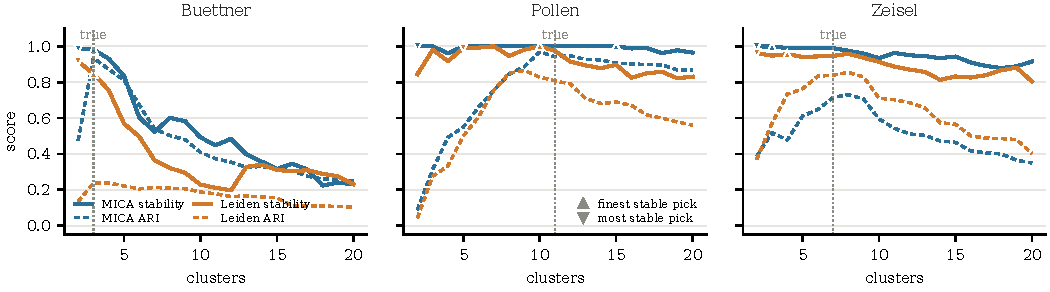
\includegraphics[width=\textwidth]{figures/a4_stability_curve.pdf}
\caption{Stability and accuracy against the number of clusters, for MICA and Leiden on three datasets,
from the confirmatory runs on matched candidates (medians over seeds 3 to 9, 25 subsamples). Solid lines
are the stability score the rule reads, and need no labels. Dashed lines are the ARI against the
reference labels. Triangles mark the counts the two readings picked, as a median over the seeds, and the
dotted line the true number of types. Where the solid line is flat, the rule has no basis for preferring
one setting over another, and its tie-break decides instead.}
\label{fig:curve}
\end{figure*}

\subsection{Where the choice is ambiguous}\label{sec:ambiguous}
Figure~\ref{fig:curve} shows the three shapes a stability curve takes. On Buettner MICA's stability falls
as clusters are added and the rule finds a clear maximum near the truth. On Pollen it stays at its
maximum across most of the range, leaving the threshold nothing to act on. On Zeisel it is nearly flat from 2 to
7 clusters, and its narrow intervals let the rule settle on 2 or 3, well below the truth. The flat top is mostly MICA's and sits in the smallest datasets (C3). On the five
datasets of at most 317 cells, \V{C3.five_smallest.mica.share} of MICA's settings score within 0.01 of its
best, against \V{C3.four_larger.mica.share} on the four larger ones and \V{C3.five_smallest.leiden.share}
for Leiden. When scores tie, the reading decides, and it moves MICA more (C2): the finest and plain-maximum
picks differ by \V{C2.mica} per dataset for MICA, \V{C2.leiden} for Leiden and \V{C2.kmeans} for $k$-means
(\V{A3.C2.mica} against \V{A3.C2.leiden} at seeds 0 to 2). A partition that reproduces perfectly need not be the right one, as
Ben-David, von Luxburg and P\'al showed for stability in general \cite{BenDavid2006Sober}, and von
Luxburg notes that stability becomes trivial when the perturbation is too small to change the clustering
\cite{vonLuxburg2010Stability}. On a few hundred cells, removing a fifth may be too small a change, which a test on smaller pools drawn from larger datasets could settle (Section~\ref{sec:conclusion}).

\begin{figure}[t]
\centering
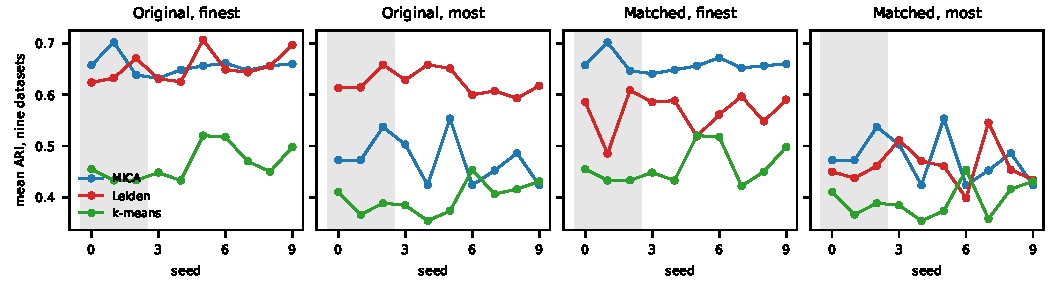
\includegraphics[width=\columnwidth]{figures/a4_seed_means.pdf}
\caption{Mean ARI over the nine small datasets at each seed, matched and original candidates, both readings,
original protocol (S0). Seeds 0 to 2 (shaded) are the exploratory runs, rerun under protocol
v1. A ranking read from one seed can differ from the ranking over ten.}
\label{fig:seeds}
\end{figure}

The subsample draw is the other source of ambiguity (Figure~\ref{fig:seeds}). Across the seven new seeds,
MICA's finest-stable mean ranges from \V{S0.mid.F.mica.seedmin} to \V{S0.mid.F.mica.seedmax} and Leiden's
from \V{S0.mid.F.leiden.seedmin} to \V{S0.mid.F.leiden.seedmax}. Per dataset, the draw moves Leiden's
finest-stable ARI by \V{range.F.leiden.mean} on average and MICA's by \V{range.F.mica.mean}. Under the plain
maximum it moves MICA's by \V{range.M.mica.mean} and Leiden's by \V{range.M.leiden.mean}, as much as
\V{range.M.leiden.max} on \V{range.M.leiden.maxds}. Under the plain maximum a ranking read from any one seed
can point either way.

\begin{table*}[t]
\centering
\caption{PBMC14K, the one large benchmark dataset and the only one in MICA's graph mode, at five seeds. ARI of the chosen partition, median over the seeds, with the range of chosen counts. MICA's node2vec and Louvain take no seed, so every MICA run is a new draw. S0 keeps the co-clustering on a random 3,000 of the 13,605 cells and uses the first 25 subsamples, S1 the same cells and all 100, S2 all cells and all 100, S3 chooseR's code on all cells and all 100. The true number of types is 7.}
\label{tab:pbmc}
\footnotesize
\setlength{\tabcolsep}{4pt}
\begin{tabular}{llcccc}
\toprule
 & & \multicolumn{2}{c}{Original grids} & \multicolumn{2}{c}{Matched candidates} \\
\cmidrule(lr){3-4}\cmidrule(lr){5-6}
Method & Scorer & Finest & Most & Finest & Most \\
\midrule
MICA & S0 & 0.624\,(5) & 0.624\,(5) & 0.395\,(4\textrm{-}5) & 0.395\,(4\textrm{-}5) \\
 & S1 & 0.625\,(5) & 0.625\,(5) & 0.395\,(4\textrm{-}5) & 0.395\,(4\textrm{-}5) \\
 & S2, all cells & 0.624\,(5) & 0.624\,(5) & 0.395\,(4\textrm{-}5) & 0.395\,(4\textrm{-}5) \\
 & S3, chooseR & 0.840\,(8) & n/a & 0.590\,(4\textrm{-}5) & n/a \\
\midrule
Leiden & S0 & 0.397\,(4) & 0.397\,(4) & 0.397\,(4) & 0.397\,(4) \\
 & S1 & 0.397\,(4) & 0.397\,(4) & 0.397\,(4) & 0.397\,(4) \\
 & S2, all cells & 0.397\,(4) & 0.397\,(4) & 0.397\,(4) & 0.397\,(4) \\
 & S3, chooseR & 0.397\,(4) & n/a & 0.397\,(4) & n/a \\
\midrule
$k$-means & S0 & 0.094\,(2\textrm{-}5) & 0.094\,(2) & 0.385\,(4\textrm{-}5) & 0.385\,(4) \\
 & S1 & 0.094\,(2) & 0.094\,(2) & 0.385\,(4) & 0.385\,(4) \\
 & S2, all cells & 0.094\,(2) & 0.094\,(2) & 0.385\,(4) & 0.385\,(4) \\
 & S3, chooseR & 0.094\,(2) & n/a & 0.440\,(5\textrm{-}6) & n/a \\
\bottomrule
\end{tabular}
\end{table*}


\subsection{PBMC14K}\label{sec:pbmc}
PBMC14K has 13,605 cells, which puts MICA in graph mode, where its node2vec and Louvain take no seed, so every
run is a new draw (Table~\ref{tab:pbmc}). MICA's graph mode never gives fewer than 4 clusters here, so the
matched counts start at 4, and the rule mostly takes that floor. Under the plain maximum on matched
candidates MICA's median is \V{pbmc.S0.mid.M.mica} at \V{pbmc.S0.mid.M.mica.k} clusters and Leiden's
\V{pbmc.S0.mid.M.leiden} at \V{pbmc.S0.mid.M.leiden.k}, within 0.02 of each other at \V{C4.ties} seeds (C4),
and $k$-means picks 4 as well. At seed 4 MICA takes 5 clusters and leads. The tie depends on which
setting stands for a count, a check the protocol left exploratory. Offered its lowest setting per count, or
every setting, Leiden takes a 5-cluster partition that reproduces perfectly at three of the five seeds, and
its median rises to \V{pbmc.S0.low.M.leiden} against MICA's \V{pbmc.S0.low.M.mica}. Seed by seed, the two
then tie at only one seed with the lowest setting, but still at three with every setting. With all 100
subsamples on the same 3,000 cells (S1), Leiden takes that partition at only two seeds, the medians are
level again, and the two tie at three or more seeds under every variant. Scored on all cells (S2), the
lowest setting still leaves only two ties. Under chooseR's reading MICA
takes 5 clusters on matched candidates at one seed with 25 subsamples and at two with 100, whether the
co-clustering is kept on 3,000 cells (S1) or uses all cells (S2), so its median stays at
\V{pbmc.S1.mid.F.mica}, while Leiden stays at 4. Under chooseR's code MICA takes 5 clusters at three seeds,
a median of \V{pbmc.S3G.mid.F.mica} against Leiden's \V{pbmc.S3G.mid.F.leiden}.

On the original grids the implementation of the rule decides MICA's choice. Our scorer on all cells picks
\V{pbmc.S2.original.F.mica.k} clusters at an ARI of \V{pbmc.S2.original.F.mica}, and chooseR's code, on the
same partitions and subsamples, picks \V{pbmc.S3G.original.F.mica.k} at \V{pbmc.S3G.original.F.mica}, close
to the 7 cell types. The reason is the resampling unit. MICA's 5-cluster partitions reproduce almost
perfectly, with medians of 0.993 to 0.999 on all cells, but with only five cluster averages to resample,
chooseR's interval for them reaches down to between 0.48 and 0.66, while ours, resampling thousands of
cells, stays within 0.004 of the median. Under chooseR's code the highest lower bound therefore comes from
a 7-cluster setting, or an 8-cluster one at seed 4, and 8 clusters clears it at every seed. Leiden's original
grid gives 4 clusters under every scorer and at every seed, and that of $k$-means gives 2 in every run in
Table~\ref{tab:pbmc} but one.
So on the original grids MICA leads Leiden on PBMC14K under every scorer and at every seed, the reverse of the plain-maximum result on the small datasets. Under our scorer the cause is the same, with the roles swapped. MICA's own grid stops at a resolution of 4.0 and gives no fewer than 5 clusters at any seed we ran, while Leiden's reaches 4. Matching adds MICA's 4-cluster partitions, and the plain maximum takes one at four of the five seeds, which levels the two.

% Written by scripts/large_scale/make_tables.py from results/large_scale/. Do not edit by hand.
\begin{table*}[t]
\centering
\caption{The Allen whole mouse brain atlas, 2,341,350 cells by 30,520 genes after preprocessing. Full data: the method ran on every cell. Sample: a uniform random 100,000-cell sample, the only size at which MICA runs on our machine, scored on those cells. Sample and assigned: every other cell takes the majority cluster of its 15 nearest sample cells in the full-data principal components, scored on every cell. Each method is set to the 34 classes, except Leiden's default. Time is the clustering itself, after the shared preprocessing (6 min, at most 56~GB). Peak memory sums a stage's processes, an upper bound when forked workers share memory: no single process used more than 18~GB. Sample times and memory are from the whole-job pilot runs, where Leiden's time includes a sweep of 200 resolutions. The assignment rows add only the neighbour search and vote.}
\label{tab:large}
\footnotesize
\setlength{\tabcolsep}{4pt}
\begin{tabular}{llrrrrr}
\toprule
Method & Setting & Clusters & ARI & AMI & Time & Peak memory \\
\midrule
\multicolumn{7}{l}{\textit{Full data, 2,341,350 cells}} \\
PCA + $k$-means & $k = 34$ & 34 & 0.590 & 0.818 & 80 s & 2~GB \\
PCA + Leiden & resolution 0.05 & 31 & 0.748 & 0.873 & 3 min & 59~GB \\
PCA + Leiden & resolution 1.0 (default) & 93 & 0.522 & 0.830 & 3 min & 59~GB \\
\midrule
\multicolumn{7}{l}{\textit{Sample, 100,000 cells}} \\
PCA + $k$-means & $k = 34$ & 34 & 0.579 & 0.820 & 46 s & 27~GB \\
PCA + Leiden & resolution 0.17 & 35 & 0.661 & 0.850 & 17 min & 27~GB \\
MICA, graph mode & resolution 3.2 & 33 & 0.652 & 0.836 & 7.1 h & 140~GB \\
\midrule
\multicolumn{7}{l}{\textit{Sample and assigned, 2,341,350 cells}} \\
PCA + $k$-means & $k = 34$ & 34 & 0.584 & 0.826 & 79 s & 2~GB \\
PCA + Leiden & resolution 0.17 & 35 & 0.661 & 0.850 & 79 s & 2~GB \\
MICA, graph mode & resolution 3.2 & 33 & 0.657 & 0.840 & 79 s & 2~GB \\
\bottomrule
\end{tabular}
\end{table*}


\subsection{The Allen atlas at full scale}\label{sec:large}
After preprocessing the atlas has \V{large.n_cells} cells by \V{large.n_genes} genes, and the PCA pipelines
use \V{large.n_hvg} of those genes, reduced to \V{large.n_pcs} components (Table~\ref{tab:large}). Both
pipelines ran on every cell. The whole run, with \V{large.kmeans.n_seeds} $k$-means seeds and
\V{large.leiden.n_runs} Leiden runs, took \V{large.full.minutes_cached} minutes. The raw files were already
cached, because the check on the 100,000-cell sample had just read them. Reading the 13 files from disk took
\V{large.read.minutes_cold} minutes in that check, so the same run from the disk takes about
\V{large.full.minutes_disk}. No single process used more than \V{large.max_process_gb}~GB, though the
processes running side by side held up to \V{large.full.max_gb}~GB together. Set to the 34 classes, $k$-means reaches an ARI of \V{large.kmeans.ari} on
all cells at seed 0, and \V{large.kmeans.ari_seeds} over three seeds. Leiden, at the resolution whose count
is closest to 34, reaches \V{large.leiden.ari} with \V{large.leiden.k} clusters at seed 0, and
\V{large.leiden.ari_seeds} over three seeds. At seed 0 no resolution we ran gave exactly 34:
\V{large.leiden.res} gave \V{large.leiden.k} and \V{large.leiden.runnerup.res} gave
\V{large.leiden.runnerup.k}, neighbours on the grid, and the ARI broke the tie, \V{large.leiden.ari} against
\V{large.leiden.runnerup.ari}. At Scanpy's default resolution, which needs no labels, Leiden gives
\V{large.leiden.default.k} clusters and an ARI of \V{large.leiden.default.ari}.

The label-free checks are cheap at this size. Partitions from different seeds agree at an ARI of at least
\V{large.kmeans.seed_ari_min} for $k$-means and \V{large.leiden.seed_ari_min} for Leiden at the chosen
resolution, but at that resolution Leiden's count moved from \V{large.leiden.k_seeds} clusters across the
three seeds (check 5 in Table~\ref{tab:checks}). A setting also means something different at another size.
Resolution \V{large.leiden.pilot_res}, the pick on the 100,000-cell sample, gives \V{large.sample.leiden.k}
clusters there and \V{large.leiden.k_at_pilot_res} on all cells. A setting tuned on a sample does not carry
over to the full data, and the full-data and sample results for Leiden are not at the same setting.

MICA ran only on the sample. There it took \V{large.mica.hours} hours and \V{large.mica.peak_gb}~GB and
reached \V{large.sample.mica.ari} with \V{large.sample.mica.k} clusters, level with Leiden's
\V{large.sample.leiden.ari} on the same cells and ahead of $k$-means' \V{large.sample.kmeans.ari}. Giving
the other \V{large.n_assigned} cells the cluster of their nearest sample cells took about
\V{large.assign.seconds} seconds and scores \V{large.assigned.mica.ari} on all cells. Within the sample, the
vote gave a held-out cell its own MICA cluster \V{large.holdout.mica.acc} percent of the time, which needs
no labels and says the assignment step adds little error. The result is still an approximation. MICA
never saw \V{large.unseen_pct} percent of the cells, and the assignment works in the principal components
rather than MICA's own distance. Extended the same way, the baselines' sample partitions score
\V{large.assigned.kmeans.ari} and \V{large.assigned.leiden.ari} on all cells. Compared through the same
sample, then, MICA and Leiden are level and both are ahead of $k$-means, whether the sample alone or all
cells after assignment are scored. Leiden run on every cell, at its own setting, reaches
\V{large.leiden.ari}.

\subsection{Secondary rules, at the exploratory seeds}\label{sec:transfer}
These ran at seeds 0 to 2 or at one seed and were not repeated (Appendices~\ref{app:rulesall},
\ref{app:secondary} and \ref{app:transfer}). MICA's best mean there, 0.727, came from its
shipped default of four clusters, which is what tuning $k$ on the other datasets' labels picks in 26 of 27
held-out choices, so it carries label information about this benchmark rather than evidence for the method.
For PCA plus Leiden, the resolution tuned on the other datasets lifted the mean from 0.514 under its shipped default to 0.641. The silhouette rule on matched
candidates gave MICA 0.593 against 0.478 in the principal components, but MICA trailed in its own embedding,
0.493 against 0.497. On a pool of 2,500 PBMC14K cells, drawn afresh at each of three seeds, the two readings of the rule
differed on 3 of 3 pools in MICA's small-data mode and on none in graph mode. On matched candidates that
became 2 of 3 against 1 of 3, too few to call a mode effect (Appendix~\ref{app:modesize}).

\subsection{Cost}\label{sec:cost}
Choosing a setting costs far more than clustering at one, and a user pays both. On the small datasets, one
subsample of protocol v1 took a median of \V{cost.small.mica.median}~s for MICA's whole sweep of $k$,
\V{cost.small.leiden.median}~s for Leiden's sweep and \V{cost.small.kmeans.median}~s for $k$-means, so a
full run of 100 subsamples takes minutes per dataset, and cost is no reason to prefer a method there. On
PBMC14K one MICA subsample takes a median of about five to six minutes, depending on the seed, almost all
of it node2vec, against 75 to 90 seconds for Leiden and $k$-means together, so one run of 100 subsamples took 8 to 10 hours for MICA and 2 to 2.5 for the two baselines. That cost is why the selection rule's evidence on a large dataset rests on PBMC14K alone, and why the
Allen atlas compares the methods at a fixed number of clusters (Section~\ref{sec:large}). chooseR's own scoring adds under a minute per
small dataset and seed.

\section{Discussion}\label{sec:discussion}
% Written by hand. Every number is a \V{} value from numbers_a4.tex (scripts/a4_protocol_v1.py).
\begin{table}[t]
\centering
\caption{What the experiments support. Confirmed means the effect met its criterion at the seven new
seeds under the protocol fixed in advance (Table~\ref{tab:criteria}). Exploratory means it was measured on
the same runs but given no criterion in advance.}
\label{tab:effects}
\footnotesize
\setlength{\tabcolsep}{3pt}
\begin{tabular}{>{\raggedright\arraybackslash}p{2.75cm}>{\raggedright\arraybackslash}p{3.15cm}>{\raggedright\arraybackslash}p{1.75cm}}
\toprule
Effect & Evidence (mean ARI) & Status \\
\midrule
The candidates decide the plain-maximum ranking & Own grids: Leiden \V{S0.original.M.leiden}, MICA \V{S0.original.M.mica}. Matched: \V{S0.mid.M.leiden} against \V{S0.mid.M.mica} & Confirmed (C5) \\
The reading moves MICA most & Mean change between readings: MICA \V{C2.mica}, Leiden \V{C2.leiden}, $k$-means \V{C2.kmeans} & Confirmed (C2) \\
Flat scores sit with MICA on the smallest datasets & Share tied at the top: \V{C3.five_smallest.mica.share} against \V{C3.four_larger.mica.share} & Confirmed (C3) \\
MICA ahead on matched candidates, chooseR's reading & \V{S0.mid.F.mica} against \V{S0.mid.F.leiden}, at \V{C1.F.leads} seeds, but \V{E5.S0.mid.F.loo} without Buettner & Mean only (C1) \\
MICA ahead on matched candidates, plain maximum & \V{S0.mid.M.mica} against \V{S0.mid.M.leiden}, ahead at \V{C1.M.leads} seeds & Not supported (C1) \\
Our scorer computes chooseR's co-clustering & \V{FC.identical} of \V{FC.matrices} matrices identical & Confirmed (FC) \\
The setting behind each count matters & Leiden, plain maximum: \V{variants.M.leiden.min} to \V{variants.M.leiden.max} across variants & Exploratory \\
The number of subsamples matters & Plain maximum, matched: level at 25, \V{S1.mid.M.mica} against \V{S1.mid.M.leiden} at 100 & Exploratory \\
The interval decides choices & chooseR's code chooses nothing in \V{S3.nochoice.mica} MICA runs & Exploratory \\
\bottomrule
\end{tabular}
\end{table}


\textbf{What the experiments support.} Table~\ref{tab:effects} sorts the effects by the strength of the
evidence behind them. The effects of the candidates and of the reading, and where MICA's flat scores sit,
held at seven new seeds against criteria fixed in advance. The effects of the number of subsamples, the
interval and the setting per count were measured on the same runs but not fixed in advance. Leiden's lead
on its own grid under the plain maximum is our sturdiest result: on the nine small datasets it holds at
every seed, without any one dataset and at either number of subsamples, and matching the counts removes
it. On
PBMC14K the original grids favour MICA instead, \V{pbmc.S0.original.M.mica} against
\V{pbmc.S0.original.M.leiden}, because there it is MICA's own grid that cannot reach 4 clusters. The
reading moved MICA more than the baselines, and MICA's flat scores stayed in the smallest datasets. The
effects on the methods held only in part. MICA's lead on matched candidates under chooseR's reading held at
every new seed, but MICA has the higher median on only \V{E5.S0.mid.F.micawins} of the nine datasets and
Leiden on \V{E5.S0.mid.F.leidenwins}, and with 25 subsamples the mean lead rests on Buettner. Under the
plain maximum with 25 subsamples there is no lead to report. So this benchmark says more about
how the evaluation shapes a ranking than about which method clusters better.

\textbf{Why the rankings change.} Four mechanisms account for what we saw, and each was measured rather
than assumed. The first is the menu. A rule can only pick from what it is shown, and Leiden's original
grid never produced some of the counts the plain maximum prefers. PCA plus $k$-means shows the size of
this effect. It shares Leiden's representation, so the gap between those two reflects the menu and the
clustering step, and under the plain maximum that gap shrinks from \V{E2.original.M.leidenminuskmeans} on
the original grids to \V{E2.mid.M.leidenminuskmeans} once the counts are matched. It shares MICA's menu
and clustering step, so the gap between those two reflects the representation, and that gap barely
moves, \V{E2.original.M.micaminuskmeans} against \V{E2.mid.M.micaminuskmeans}. The candidates removed
Leiden's lead, while the representation contributed about the same in both designs, though
under the plain maximum that contribution rests on Usoskin. Haslbeck and Wulff found that a stability
estimate depends on its candidate range in the same way \cite{Haslbeck2020Corrected}.

The second mechanism is ties. When many settings reproduce almost perfectly, stability no longer
separates them and the tie-break decides, toward fewer clusters under the plain maximum and toward more
under chooseR's reading. Ben-David et al. showed that stability alone cannot tell such settings apart
\cite{BenDavid2006Sober}, and here it is mostly MICA's problem. Its distance between two cells does not
change when the sample does, and on the five smallest datasets \V{C3.five_smallest.mica.atone} percent of its settings
reproduce perfectly, against \V{C3.four_larger.mica.atone} percent on the four larger datasets and
\V{C3.five_smallest.leiden.atone} percent of Leiden's. A perturbation too small to change the clustering makes
stability trivial \cite{vonLuxburg2010Stability}, which may be why MICA's scores are flat where Leiden's are
not.

The third is the interval. The threshold is the highest lower bound among the candidates, so how the
interval is computed decides which settings clear it. A coarse partition that reproduces perfectly is
where the two implementations part most. Under ours its lower bound is 1.0 and becomes the threshold, so
only a finer setting that also reproduces perfectly clears it. Leiden on Klein had none. Under chooseR's
code it gets no interval at all, and a single such candidate leaves the threshold undefined, so the code
as written makes no choice in most MICA runs. Resampling clusters also gives wide intervals when there
are only a few clusters, and on PBMC14K that alone moved MICA's choice on its original grid from
\V{pbmc.S2.original.F.mica.k} clusters to \V{pbmc.S3G.original.F.mica.k}. The fourth mechanism is the
number of subsamples, which left the matched finest-stable comparison unchanged in direction but turned
the matched plain-maximum comparison from level into a MICA lead, and the original-grid finest-stable
comparison from level into a narrow MICA lead that rests on Buettner.

% Written by hand. Every number is a \V{} value from numbers_a4.tex (scripts/a4_protocol_v1.py).
\begin{table*}[t]
\centering
\caption{Checks before trusting a comparison of clustering methods under a label-free selection rule. The
first six need no labels, so a user can run them on new data. They ask whether the rule's choice is
determined by the data. The last five need reference labels, so they judge a benchmark: whether its
ranking of methods holds up. Our runs are the confirmatory runs on the nine small datasets (matched
candidates, 25 subsamples, seeds 3 to 9) unless stated.}
\label{tab:checks}
\footnotesize
\setlength{\tabcolsep}{3pt}
\renewcommand{\arraystretch}{1.1}
\begin{tabular}{>{\raggedright\arraybackslash}p{2.5cm}>{\raggedright\arraybackslash}p{3.1cm}>{\raggedright\arraybackslash}p{3.0cm}>{\raggedright\arraybackslash}p{3.7cm}>{\raggedright\arraybackslash}p{5.1cm}}
\toprule
Check & Needs & Detects & How to read it & In our runs \\
\midrule
\multicolumn{5}{l}{\textit{On unlabeled data: is the choice determined by the data?}} \\
1. Same candidate counts & The cluster counts each method's settings reach on the full data & A menu that favours one method & If the ranges differ, match them, or the ranking partly reflects the menu & Leiden's own grid skips counts the plain maximum prefers. Matching moved its mean from \V{S0.original.M.leiden} to \V{S0.mid.M.leiden} \\
2. Scores not flat & The stability score of every setting & Settings the rule cannot tell apart & If most settings tie at the top, the tie-break chooses, and the count is unresolved & Share within 0.01 of the best: MICA \V{C3.five_smallest.mica.share} on the five smallest datasets, \V{C3.four_larger.mica.share} on the four larger, Leiden \V{C3.five_smallest.leiden.share} \\
3. Readings agree & The count each reading picks & The tie-break setting the count & Picks several clusters apart mean the count is unresolved & Picks \V{L.gap} or more clusters apart in \V{L.disagree.n} of \V{L.runs} runs, \V{L.disagree.mica} of them MICA's \\
4. Pick inside the range & The chosen count and the smallest count offered & A coarse partition that reproduces perfectly pinning the rule & A pick at the floor says nothing finer was stable, not that the floor is right & \V{L.floor.F.n} of \V{L.runs} finest-stable picks and \V{L.floor.M.n} plain-maximum picks sit at the floor \\
5. Count stable across draws and settings & The chosen count at several seeds, and with another setting standing for each count & A choice that depends on the draw or on the menu & Report the range of counts, not one count & Leiden on Pollen, plain maximum: \V{L.pollen.leiden.kM} clusters across seeds. PBMC14K: Leiden's pick moves from \V{pbmc.S0.mid.M.leiden.k} to \V{pbmc.S0.low.M.leiden.k} clusters when its lowest setting stands for each count \\
6. Rule defined and stable across implementations & Whether the interval can be formed, and the pick under other subsample numbers or bootstraps & An undefined rule, or one that its details decide & A rule that cannot choose needs a repair, and the repair is a new rule & chooseR's code chooses nothing in \V{S3.nochoice.mica} MICA runs (every seed and dataset). Our scorer and chooseR's code pick the same count in \V{E4.mid.mica.same} MICA and \V{E4.mid.leiden.same} Leiden runs \\
\midrule
\multicolumn{5}{l}{\textit{With reference labels: does a benchmark's ranking hold?}} \\
7. Both readings & Mean ARI per method under each reading & A ranking made by the tie-break & A ranking that flips between readings is a property of the rule & MICA ahead under chooseR's reading, \V{S0.mid.F.mica} against \V{S0.mid.F.leiden}. Level under the plain maximum, \V{S0.mid.M.mica} against \V{S0.mid.M.leiden} \\
8. Across draws & Mean ARI per method at each seed & A ranking made by one draw & Count the seeds each method leads at & MICA ahead at \V{C1.F.leads} seeds under chooseR's reading, \V{C1.M.leads} under the plain maximum \\
9. Across implementations & Mean ARI per method under each scorer & A ranking made by the rule's details & The ranking should keep its direction & Plain maximum, matched: level with 25 subsamples, MICA ahead with 100, \V{S1.mid.M.mica} against \V{S1.mid.M.leiden} \\
10. Across settings per count & Mean ARI per method with each setting standing for a count & A ranking made by the menu & The ranking should keep its direction & PBMC14K: a tie at \V{C4.ties} seeds, but Leiden's median moves from \V{pbmc.S0.mid.M.leiden} to \V{pbmc.S0.low.M.leiden} with its lowest setting \\
11. Without each dataset & Mean ARI per method leaving out one dataset at a time & A mean carried by one dataset & The sign of the gap should survive & MICA's lead under chooseR's reading becomes \V{E5.S0.mid.F.loo} without Buettner \\
\bottomrule
\end{tabular}
\end{table*}


\textbf{What to check before trusting a comparison.} The mechanisms suggest checks, and they come in two
kinds (Table~\ref{tab:checks}). Checks 1 to 6 need no labels. They ask whether the menu is fair and the
rule's choice is determined by the data, from things a user can see on new data: the counts each method can reach, the
stability scores, the count each reading picks and how it moves across draws, settings and
implementations. Checks 7 to 11 need reference labels. They ask whether a benchmark's ranking of methods
holds up, and so they are for whoever builds or reads a benchmark, not for a user facing unlabeled data. A
label-free check can only say that a choice is not determined, never that it is right, and a benchmark
check can only show that a ranking is fragile. Within what we tested, no comparison passes all eleven, so
we have not shown that passing them is enough. Our matched finest-stable comparison passes checks 1, 8 and
10, and check 9 once chooseR's failed intervals are repaired. It passes check 11 only with 100 subsamples.
It fails check 2 on the five smallest datasets and check 6, since chooseR's code as written makes no choice
in most MICA runs and the chosen count moves with the number of subsamples in \V{L.moved.leiden} Leiden and
\V{L.moved.mica} MICA runs. Its lead also disappears under the plain maximum with 25 subsamples (check 7). We therefore read it as a lead for MICA under chooseR's reading on
these datasets, not as evidence that mutual information clusters better in general. A benchmark should also
report the chosen number of clusters beside any score, because a respectable ARI can come with a badly
wrong count.

\textbf{Spotting an unreliable choice without labels.} Take MICA on Pollen in the confirmatory runs on
matched candidates and suppose the labels were unknown. Two signs are visible before any comparison with labels. The stability
scores are flat at the top: \V{L.pollen.mica.share} percent of the settings lie within 0.01 of the best,
with the tied settings running from \V{L.pollen.mica.tiedlo} to \V{L.pollen.mica.tiedhi} clusters
(Figure~\ref{fig:curve}, middle). And the two
readings disagree: chooseR's reading picks \V{L.pollen.mica.kF} clusters and the plain maximum picks
\V{L.pollen.mica.kM}, the smallest count offered (checks 2, 3 and 4). Either sign says that the data do not determine the count, so the
tie-break does. The labels confirm the warning. Pollen has \V{L.pollen.mica.truek} cell types, and the two
picks score an ARI of \V{L.pollen.mica.ariF} and \V{L.pollen.mica.ariM}. The same signs fire for MICA on
Yan and on Chung, where both picks score below 0.5. Across all \V{L.runs} confirmatory runs on matched candidates on the small
datasets, the readings picked counts \V{L.gap} or more apart in \V{L.disagree.n} runs, and in those runs the
two picks differed in ARI by \V{L.disagree.arigap} on average, against \V{L.agree.arigap} in the other
runs. A pick at the smallest count offered is another sign (check 4). Such picks averaged an ARI of
\V{L.floor.F.ari} under chooseR's reading, against \V{L.interior.F.ari} for picks inside the range. The
signs are warnings, not guarantees. Leiden on Buettner shows no flat top and its readings agree, yet its
picks score only \V{L.buettner.leiden.ariF} and \V{L.buettner.leiden.ariM}. Other checks do hint at
trouble there. Its plain-maximum pick sits at the floor in \V{L.buettner.leiden.floorM} runs (check 4), and
chooseR's code picks a different count from ours in \V{L.buettner.leiden.impl} (check 6). Passing checks 2
and 3 is not enough.

\textbf{Limitations.} The main rule and its two readings come from one family, subsampling stability, and
the benchmark datasets from one source, nine of them small. Other label-free rules, such as significance tests, may rank the
methods differently. The matched design was introduced after we had seen the exploratory results. Its
conclusions are now tested at new seeds under a protocol tagged in advance, but the criteria were written
knowing the results at seeds 0 to 2, and the per-dataset analysis and the label-free signs above were
added afterwards. The protocol also left exploratory the effects of the number of subsamples, the interval
and the setting per count, so these still need runs of their own. C4 counts PBMC14K seeds 0 to 2 as well,
which we had seen before the protocol, and their three ties alone would satisfy it. Of the two new seeds,
one ties and one gives MICA the lead. MICA's graph mode never gives fewer than 4 clusters on PBMC14K, so
the matched comparison there starts at 4, and its node2vec and Louvain take no seed, so its runs cannot be
repeated exactly. The $k$-means control isolates the representation only in MICA's small-data mode. The
repairs for chooseR's failed intervals are ours, though both were declared before the runs. On the Allen
atlas the selection rule itself was not run, since subsampling MICA there is out of reach, and MICA's
result there is an approximation from a sample (Section~\ref{sec:large}). The secondary rules remain at
three seeds or one.

\section{Conclusion}\label{sec:conclusion}
When one label-free rule chooses the setting for every method, the ranking it produces depends on more
than the methods. On the nine small datasets of the scMINER benchmark the candidates decided the
plain-maximum ranking: Leiden led on its own grid, and the two methods were level once offered the same
counts. The reading of the scores and the number of subsamples also moved the ranking, and the bootstrap
interval moved individual choices. The effects of the candidates and of the reading held at seven new seeds
against criteria fixed in advance, while those of the number of subsamples and of the interval were
measured without them. Between the methods, MICA's lead under chooseR's reading on matched candidates held
at every seed, but MICA has the higher median on only \V{E5.S0.mid.F.micawins} of the nine datasets, and
with 25 subsamples the mean lead rests on one of them. PCA plus $k$-means,
the textbook baseline, scored lowest in every design on the nine small datasets. On PBMC14K, MICA and
Leiden tie on matched candidates under the plain maximum at \V{C4.ties} seeds, but the tie depends on which
setting stands for each count. On 2.3 million cells both PCA pipelines run on every cell, while MICA has
to be approximated from a sample.

The answer to our question is therefore practical. A comparison of clustering methods under label-free
selection should report the cluster counts each method can reach and match them, report the setting
behind each count, and report the count each method chose. A user facing unlabeled data can check whether
the scores are flat, whether the two readings agree, whether the pick sits at the smallest count offered, and
whether the choice survives another draw and another implementation of the rule. Whoever builds a
benchmark should also check, with the labels, that the ranking holds under both readings, across draws,
across implementations, with another setting standing for each count, and without each dataset. Where a check fails, the comparison shows at most a lead
under that rule on those datasets.

Three things remain open. Drawing pools of 150 and 300 cells from Zeisel and PBMC14K would test whether
MICA's flat scores come from small samples or from the datasets. Rules of another family, such as
significance tests, may rank the methods differently. And the stability rule itself could be run on the
Allen atlas at subsample sizes all three methods can afford.

\section*{Author contributions}
Utshab Kumar Ghosh designed and ran the experiments, wrote the code, and wrote the methods, design,
results and discussion. Laraib Khan wrote the introduction and related work and checked that the discussion
follows from the results. Rhea Eckman checked every number against the saved results and kept the
provenance and seed records.

\section*{Code and data}
The code, the saved results of every run, the tagged protocol and the scripts that rebuild every table and
figure are at \url{https://github.com/utshabkg/scminer-clustering} (Appendix~\ref{app:repro}). The ten
benchmark inputs are the scMINER authors' release, \url{https://doi.org/10.5281/zenodo.15040179}, and the
Allen atlas is public \cite{yao2023allen}.


% \balance removed: with appendices after the references it overfilled an appendix column
\bibliographystyle{IEEEtran}
\bibliography{references}

\appendices
\section{Code and data}\label{app:links}
The code and the per-run results are at \url{https://github.com/utshabkg/scminer-clustering}, where the
protocol is tagged \texttt{matched-protocol-v1}. The ten benchmark inputs are the scMINER authors'
processed release, \url{https://doi.org/10.5281/zenodo.15040179}. The saved subsample partitions of
protocol v1 take 11 GB, too large for GitHub, and we share them on request.
\texttt{scripts/a4\_protocol\_v1.py} rebuilds the generated protocol v1 tables, both figures and the
protocol v1 numbers in the text from the saved result files, and
\texttt{notebooks/assignment3\_results.ipynb} does the same for the exploratory runs' displays, so they
can be checked without rerunning an experiment. \texttt{scripts/large\_scale/make\_tables.py} does the same
for the Allen atlas. Appendix~\ref{app:repro} gives the layout of those files
and the commands that produced them.

\section{The datasets}\label{app:data}
Table~\ref{tab:data} lists the ten benchmark datasets with their sizes, label counts and
sparsity. Nine fall below the 5,000 cell point at which MICA switches from its small-data
mode to its graph mode, and PBMC14K is the only one above it, which is why mode and size
move together in the runs as shipped.

\begin{table}[t]
\centering
\caption{The ten benchmark datasets, as released by the scMINER authors and used here without further preprocessing. The smallest class column is that class as a share of all cells, and the last column is the share of the matrix that is zero.}
\label{tab:data}
\footnotesize
\setlength{\tabcolsep}{4pt}
\begin{tabular}{lrrrrr}
\toprule
Dataset & Cells & Genes & Types & Smallest (\%) & Zeros (\%) \\
\midrule
Yan & 124 & 20,286 & 8 & 2.4 & 38 \\
Goolam & 124 & 23,571 & 5 & 4.8 & 46 \\
Buettner & 182 & 8,989 & 3 & 31.9 & 38 \\
Pollen & 249 & 6,982 & 11 & 2.8 & 25 \\
Chung & 317 & 10,897 & 4 & 7.9 & 96 \\
Usoskin & 622 & 16,383 & 4 & 13.0 & 78 \\
Kolodziejczyk & 704 & 13,698 & 3 & 22.6 & 37 \\
Klein & 2,717 & 24,175 & 4 & 11.2 & 66 \\
Zeisel & 2,903 & 14,890 & 7 & 3.3 & 76 \\
PBMC14K & 13,605 & 8,846 & 7 & 13.5 & 94 \\
\bottomrule
\end{tabular}
\end{table}


\begin{table}[t]
\centering
\caption{MICA on the authors' released inputs, all genes, scored by the paper's rule (the true number of types is given and the labels pick the setting). ARI.}
\label{tab:repro}
\footnotesize
\setlength{\tabcolsep}{3.5pt}
\begin{tabular}{lrcccc}
\toprule
 & & \multicolumn{2}{c}{MICA} & Scanpy & Leiden \\
\cmidrule(lr){3-4}
Dataset & Cells & paper & ours & paper & ours \\
\midrule
Yan & 124 & 0.939 & 0.939 & 0.839 & 0.789 \\
Goolam & 124 & 0.544 & 0.544 & 0.572 & 0.308 \\
Buettner & 182 & 0.934 & 0.934 & 0.277 & 0.268 \\
Pollen & 249 & 0.942 & 0.951 & 0.874 & 0.858 \\
Chung & 317 & 0.655 & 0.655 & 0.170 & 0.319 \\
Usoskin & 622 & 0.847 & 0.835 & 0.860 & 0.598 \\
Kolodziejczyk & 704 & 1.000 & 0.727$^\ast$ & 0.996 & 0.564 \\
Klein & 2,717 & 0.980 & 0.980 & 0.820 & 0.977 \\
Zeisel & 2,903 & 0.744 & 0.764$^\dagger$ & 0.630 & 0.839 \\
PBMC14K & 13,605 & 0.853 & 0.854$^\dagger$ & 0.754 & 0.878 \\
\bottomrule
\end{tabular}
\\[2pt]
\parbox{\columnwidth}{\scriptsize $^\dagger$Graph mode, median of six runs (PBMC14K 0.850 to 0.857, Zeisel 0.755 to 0.781). Other rows use MICA's small-data mode with the final $k$-means given 100 restarts. $^\ast$Not reproduced from the released files (Sec.~\ref{sec:results}). The paper's Scanpy used 2,000 variable genes. Our Leiden uses all genes, the same input MICA gets, median of three seeds.}
\end{table}


\section{All four rules in one table}\label{app:rulesall}
Table~\ref{tab:rulesall} gives the per-dataset picks on each method's original grid under the two
stability readings, the shipped defaults and the shared-space silhouette, so the secondary rules of
Section~\ref{sec:transfer} can be read against the stability rule dataset by dataset. The plan we wrote in early October, before the stability runs, counted a win for MICA
if, under the stability rule, its median ARI was higher on at least 7 of 11 sets and higher on
average by 0.05. We later dropped that count, because the question became how the rule shapes the comparison, not whether MICA wins. It was not met on the datasets we ran:
under the stability rule MICA leads on at most 6 of the 10, one short of 7, and the eleventh set,
the Allen subset, was set aside for this rule. On the original grids the overclustering already
shows, with 19 clusters on Yan, 17 on Pollen and 11 on Chung under chooseR's reading, and the counts
move with the seed, by 3 clusters on Pollen and 1 on Yan.

\begin{table*}[t]
\centering
\caption{ARI under all four label-free rules on each method's original grid, with the chosen cluster count in parentheses and the true number of cell types after each dataset name. The choice reads no labels at run time. Default and stability values are medians over three seeds, and a pair such as (15-18) gives the smallest and largest count over those seeds. The silhouette rule was run at one seed. The mean row covers the nine small-data datasets. On PBMC14K MICA runs in graph mode, so its default there is the graph-mode resolution, 1.822 scored at 1.8, from one run made before the selection experiments, and the silhouette rule was not run. Table~\ref{tab:common} gives the stability rule on the cluster counts the baseline produces.}
\label{tab:rulesall}
\footnotesize
\setlength{\tabcolsep}{4pt}
\begin{tabular}{lcccccccc}
\toprule
 & \multicolumn{2}{c}{Default} & \multicolumn{2}{c}{Silhouette} & \multicolumn{2}{c}{Finest stable} & \multicolumn{2}{c}{Most stable} \\
\cmidrule(lr){2-3}\cmidrule(lr){4-5}\cmidrule(lr){6-7}\cmidrule(lr){8-9}
Dataset (types) & MICA & Leiden & MICA & Leiden & MICA & Leiden & MICA & Leiden \\
\midrule
Yan (8) & 0.765\,(4) & 0.845\,(5) & 0.794\,(5) & 0.765\,(4) & 0.496\,(19\textrm{-}20) & 0.845\,(5\textrm{-}8) & 0.496\,(3) & 0.765\,(4\textrm{-}5) \\
Goolam (5) & 0.582\,(4) & 0.349\,(6) & 0.630\,(2) & 0.619\,(2) & 0.593\,(6\textrm{-}7) & 0.429\,(2\textrm{-}3) & 0.630\,(2\textrm{-}3) & 0.619\,(2\textrm{-}3) \\
Buettner (3) & 0.919\,(4) & 0.237\,(4) & 0.474\,(2) & 0.154\,(2) & 0.934\,(3) & 0.232\,(3) & 0.474\,(2\textrm{-}3) & 0.134\,(2\textrm{-}3) \\
Pollen (11) & 0.493\,(4) & 0.865\,(9) & 0.942\,(12) & 0.870\,(9) & 0.898\,(15\textrm{-}18) & 0.755\,(7\textrm{-}11) & 0.087\,(2) & 0.755\,(5\textrm{-}11) \\
Chung (4) & 0.655\,(4) & 0.567\,(7) & 0.551\,(9) & 0.046\,(2) & 0.474\,(11\textrm{-}12) & 0.129\,(3\textrm{-}4) & 0.100\,(2) & 0.129\,(3) \\
Usoskin (4) & 0.839\,(4) & 0.393\,(10\textrm{-}11) & 0.347\,(2) & 0.761\,(3) & 0.818\,(3) & 0.633\,(6) & 0.818\,(3) & 0.757\,(3\textrm{-}6) \\
Kolodziejczyk (3) & 0.834\,(4) & 0.525\,(7) & 0.727\,(3) & 0.525\,(7) & 0.722\,(3\textrm{-}5) & 0.838\,(4) & 0.630\,(2) & 0.838\,(4) \\
Klein (4) & 0.980\,(4) & 0.469\,(10\textrm{-}11) & 0.501\,(2) & 0.859\,(3) & 0.501\,(2\textrm{-}3) & 0.973\,(4) & 0.501\,(2) & 0.859\,(3\textrm{-}4) \\
Zeisel (7) & 0.478\,(4) & 0.378\,(21) & 0.386\,(2) & 0.473\,(3) & 0.518\,(3) & 0.855\,(8\textrm{-}9) & 0.518\,(2\textrm{-}3) & 0.855\,(8) \\
PBMC14K (7) & 0.846\,(7) & 0.866\,(8) & n/a & n/a & 0.629\,(5) & 0.397\,(4) & 0.629\,(5) & 0.397\,(4) \\
\midrule
\textit{Mean, nine small} & \textbf{0.727} & \textbf{0.514} & \textbf{0.595} & \textbf{0.564} & \textbf{0.661} & \textbf{0.632} & \textbf{0.473} & \textbf{0.635} \\
\bottomrule
\end{tabular}
\end{table*}


\section{The stability rule on a common range}\label{app:common}
The 2 to 20 filter caps both grids without matching them. Table~\ref{tab:common} gives, for each
dataset, the span of cluster counts the baseline's resolution grid produced, and the stability
rule re-applied to MICA's saved scores restricted to the set of counts the baseline produced in
the same run. That set can have gaps: on Yan the baseline makes 2 and 4 to 8 clusters but never
3. Nothing is rerun and no labels are used to restrict, but the restriction was chosen after the
results were seen and is applied to MICA only. It is a sensitivity check on what the candidate
grids do to the ranking and not a fair comparison, which is why the matched design of
Section~\ref{sec:design} replaces it as the comparison we rely on. The largest gains in MICA's finest-stable ARI are
on Yan, where its pick falls from 19 clusters to 7 and its ARI rises from 0.496 to 0.925, and on
Klein, by 0.36. On Pollen the pick falls from 17 to the true 11 at 0.969, though 11 is also the
most clusters the baseline makes there. This check suggested a larger lead than the matched runs
give, 0.772 to 0.632 under chooseR's reading, because it held MICA to the baseline's narrow range.
Offered the full range again, MICA picks 19 or 20 clusters on Yan. Where all 19 counts were offered
in the matched runs, MICA's picks are the same as on its original grid in 8 of 8 cases.

\begin{table*}[t]
\centering
\caption{The stability rule on its own grids and on a common range. The second column is the span of cluster counts the baseline's resolution grid produced over the three seeds. MICA's $k$ covers 2 to 20 on every dataset. The middle pair re-applies the rule's own selection to MICA's saved scores restricted to the set of counts the baseline produced in the same run, which can have gaps within that span. The restriction uses no labels but was chosen after the results were seen and applies to MICA only. Values are medians over three seeds, F the finest-stable reading and M the plain maximum.}
\label{tab:common}
\footnotesize
\setlength{\tabcolsep}{4pt}
\begin{tabular}{lccccccc}
\toprule
 & & \multicolumn{2}{c}{MICA, own grid} & \multicolumn{2}{c}{MICA, common range} & \multicolumn{2}{c}{Leiden} \\
\cmidrule(lr){3-4}\cmidrule(lr){5-6}\cmidrule(lr){7-8}
Dataset (types) & Baseline span & F & M & F & M & F & M \\
\midrule
Yan (8) & 2\textrm{-}8 & 0.496 & 0.496 & 0.925 & 0.765 & 0.845 & 0.765 \\
Goolam (5) & 2\textrm{-}8 & 0.593 & 0.630 & 0.593 & 0.630 & 0.429 & 0.619 \\
Buettner (3) & 2\textrm{-}14 & 0.934 & 0.474 & 0.934 & 0.474 & 0.232 & 0.134 \\
Pollen (11) & 4\textrm{-}11 & 0.898 & 0.087 & 0.969 & 0.549 & 0.755 & 0.755 \\
Chung (4) & 2\textrm{-}11 & 0.474 & 0.100 & 0.477 & 0.512 & 0.129 & 0.129 \\
Usoskin (4) & 3\textrm{-}18 & 0.818 & 0.818 & 0.818 & 0.818 & 0.633 & 0.757 \\
Kolodziejczyk (3) & 4\textrm{-}12 & 0.722 & 0.630 & 0.722 & 0.722 & 0.838 & 0.838 \\
Klein (4) & 3\textrm{-}17 & 0.501 & 0.501 & 0.863 & 0.863 & 0.973 & 0.859 \\
Zeisel (7) & 3\textrm{-}20 & 0.518 & 0.518 & 0.648 & 0.648 & 0.855 & 0.855 \\
\midrule
\textit{Mean} & & \textbf{0.661} & \textbf{0.473} & \textbf{0.772} & \textbf{0.665} & \textbf{0.632} & \textbf{0.635} \\
\bottomrule
\end{tabular}
\end{table*}


\section{Mode against size}\label{app:modesize}
Table~\ref{tab:modesize} gives the three arms of the test in Section~\ref{sec:transfer}, run at the
exploratory seeds 0 to 2. Within a
seed the cells, the subsamples and the labels are shared. The pipelines differ in their
normalisation of the mutual information and in the cluster counts their grids reach, so the test
says nothing about the mutual information distance itself. On the original grids the difference
looks like a mode effect: in small-data mode the two readings choose differently on every pool, by a
median of 0.319 ARI, and in graph mode on none. But graph mode makes few coarse partitions. On MICA's
own grid, up to a resolution of 4.0, it made no fewer than 4 or 5 clusters on these pools. Extending
the resolution to 30 lowers that floor to 4, 3 and 2 clusters, while small-data mode's $k$ reaches 2
on every pool. The matched candidates, the counts all three arms reach, start at 4, 4 and 3. On them
the difference shrinks but does not vanish. The two readings now differ on 2 of 3 pools in small-data mode, by a
median of 0.185 ARI, against 1 of 3 in graph mode and for the baseline. The tied counts span 3, 1 and 3 in small-data mode against
1, 1 and 1 in graph mode and 1, 1 and 2 for the baseline, and every arm picks 3 to 5 clusters where
there are 7 types.

\begin{table}[t]
\centering
\caption{Mode against size. One fixed pool of 2,500 PBMC14K cells, drawn afresh at each of three seeds, run through both of MICA's pipelines and the baseline under the same rule. The data, the size, the subsamples and the labels are identical across the three rows. The rows use each arm's original grid, and the cluster counts those grids reach differ: on MICA's own grid of 0.1 to 4.0, graph mode made no fewer than 4 or 5 clusters on these pools. Appendix~\ref{app:modesize} shows that the difference shrinks but does not vanish when all three arms are offered the same counts. Tied settings are those within 0.01 of the best. The span is the range of cluster counts among them, reported as the median over the three pools with the observed range. The last two columns say how often the two readings of the rule chose differently and by how much in ARI.}
\label{tab:modesize}
\footnotesize
\setlength{\tabcolsep}{4pt}
\resizebox{\columnwidth}{!}{%
\begin{tabular}{lcccc}
\toprule
Pipeline & Share tied & Span & Readings differ & Median gap \\
\midrule
MICA, small-data mode & 0.26 & 4 (2\textrm{-}5) & 3 of 3 & 0.319 \\
MICA, graph mode & 0.16 & 0 (0\textrm{-}1) & 0 of 3 & 0.000 \\
Leiden, as a control & 0.15 & 1 (1\textrm{-}1) & 1 of 3 & 0.000 \\
\bottomrule
\end{tabular}}
\end{table}


\section{The default and silhouette rules}\label{app:secondary}
The body concentrates on the stability rule's two readings. The default and the silhouette rule
carry choices of their own, and the default favours MICA for reasons that have little to do with
its clustering.

\textbf{The shipped default.}
MICA's default of four clusters leads on seven of nine datasets, and three of them have exactly
four types. We cannot show how it was chosen, but its apparent strength is a property of this
benchmark's composition rather than of the method, and the drop outside 3 to 5 types gives no reason
to expect it to carry over to tissue with many more types. The baseline's default is a resolution
rather than a count, and it overclusters badly here, reaching 21 clusters on Zeisel.

\textbf{The silhouette rule.} It depends on the space it is scored in. Scoring the same partitions in the 50
principal components rather than in MICA's own embedding changes the selected ARI by 0.13
on average for MICA and 0.16 for the baseline, reaching 0.52, with only the space changing
(Appendix~\ref{app:repro}). The order depends on it too: in MICA's own embedding MICA trails, 0.493
against 0.549 under the shared cap and 0.493 against 0.497 on matched candidates, so the lead
holds only for the 50 principal components we fixed as the shared space. In those components, on
matched candidates, the baseline's fall to 0.478 comes as it picks 2 clusters on seven of the nine
datasets.

\section{The transfer comparison}\label{app:transfer}
Table~\ref{tab:transfer} gives the transfer comparison of Section~\ref{sec:transfer} per
dataset. It uses the other datasets' labels to choose each setting, so it answers how far a
setting tuned on labelled benchmarks carries to a new one, not what a user could do without
labels. MICA's tuned $k$ is 4 on every held-out dataset except Yan at one seed, where it is 3.
The baseline's tuned resolution lies between 0.22 and 0.30 and gives 2 to 8 clusters. MICA's setting
is $k$ and the baseline's a resolution on the 300-point grid. PBMC14K takes the baseline's resolution
that is best on the nine, which gives 6 clusters at 0.786, well above either method's label-free pick. MICA's
graph mode has no setting that carries over from $k$, so MICA is not transferred there. Our early October plan proposed this rule in graph mode on Klein, Zeisel and PBMC14K.
Transferring $k$ across the nine small datasets instead compares like with like and also tests MICA's
shipped default.

\begin{table}[t]
\centering
\caption{The transfer comparison, which is not label-free. Each small dataset takes the setting with the best mean ARI over the other eight at the same seed (MICA: $k$, Leiden: a resolution), and PBMC14K takes the baseline's resolution best on the nine. MICA's graph mode has no setting that carries over from $k$. ARI with the resulting cluster count in parentheses, medians over three seeds.}
\label{tab:transfer}
\footnotesize
\setlength{\tabcolsep}{4pt}
\begin{tabular}{lcc}
\toprule
Dataset (types) & MICA & Leiden \\
\midrule
Yan (8) & 0.765\,(3\textrm{-}4) & 0.765\,(4) \\
Goolam (5) & 0.582\,(4) & 0.619\,(2) \\
Buettner (3) & 0.919\,(4) & 0.134\,(2) \\
Pollen (11) & 0.493\,(4) & 0.606\,(6\textrm{-}7) \\
Chung (4) & 0.655\,(4) & 0.510\,(6) \\
Usoskin (4) & 0.839\,(4) & 0.696\,(5) \\
Kolodziejczyk (3) & 0.834\,(4) & 0.696\,(5) \\
Klein (4) & 0.980\,(4) & 0.886\,(5) \\
Zeisel (7) & 0.478\,(4) & 0.855\,(8) \\
PBMC14K (7) & n/a & 0.786\,(6) \\
\midrule
\textit{Mean, nine small} & \textbf{0.727} & \textbf{0.641} \\
\bottomrule
\end{tabular}
\end{table}


\section{Adjusted mutual information}\label{app:ami}
Table~\ref{tab:ami} gives the AMI for the same chosen partitions as Table~\ref{tab:rulesall}.
The two measures agree on which method leads under every rule. The AMI usually sits above the
ARI when the chosen count is wrong, though not always: the baseline's 8-cluster pick on Zeisel
scores 0.855 under ARI and 0.815 under AMI. On average it sits above by 0.17 across MICA's
54 stability picks on the original grids when the rule chose too many clusters and by 0.12 when it
chose too few, which it did in 35 of them, and it can be far more forgiving of
a partition that merges types: on Pollen MICA's 17-cluster partition scores 0.898 under ARI and 0.913 under AMI, while
its 2-cluster partition scores 0.087 and 0.318. Being the stricter of the two on average, in
both directions, is why we report the ARI in the main table.

\begin{table*}[t]
\centering
\caption{Adjusted mutual information for the same chosen partitions as Table~\ref{tab:rulesall}, on the same runs. The AMI and the ARI agree on which method leads under every rule. The AMI usually sits above the ARI when the chosen count is wrong, in either direction, and it is much more forgiving of a partition that merges cell types, such as MICA's 2-cluster pick on Pollen.}
\label{tab:ami}
\footnotesize
\setlength{\tabcolsep}{4pt}
\begin{tabular}{lcccccccc}
\toprule
 & \multicolumn{2}{c}{Default} & \multicolumn{2}{c}{Silhouette} & \multicolumn{2}{c}{Finest stable} & \multicolumn{2}{c}{Most stable} \\
\cmidrule(lr){2-3}\cmidrule(lr){4-5}\cmidrule(lr){6-7}\cmidrule(lr){8-9}
Dataset (types) & MICA & Leiden & MICA & Leiden & MICA & Leiden & MICA & Leiden \\
\midrule
Yan (8) & 0.804 & 0.846 & 0.817 & 0.804 & 0.721 & 0.846 & 0.652 & 0.804 \\
Goolam (5) & 0.749 & 0.587 & 0.679 & 0.652 & 0.771 & 0.584 & 0.679 & 0.652 \\
Buettner (3) & 0.884 & 0.272 & 0.590 & 0.304 & 0.904 & 0.287 & 0.590 & 0.283 \\
Pollen (11) & 0.731 & 0.917 & 0.943 & 0.924 & 0.913 & 0.890 & 0.318 & 0.890 \\
Chung (4) & 0.762 & 0.738 & 0.725 & 0.128 & 0.709 & 0.339 & 0.292 & 0.339 \\
Usoskin (4) & 0.798 & 0.624 & 0.508 & 0.755 & 0.821 & 0.709 & 0.821 & 0.747 \\
Kolodziejczyk (3) & 0.888 & 0.723 & 0.784 & 0.723 & 0.822 & 0.896 & 0.757 & 0.896 \\
Klein (4) & 0.963 & 0.700 & 0.664 & 0.890 & 0.664 & 0.956 & 0.664 & 0.890 \\
Zeisel (7) & 0.565 & 0.644 & 0.495 & 0.580 & 0.648 & 0.815 & 0.648 & 0.815 \\
PBMC14K (7) & 0.868 & 0.893 & n/a & n/a & 0.790 & 0.725 & 0.790 & 0.725 \\
\midrule
\textit{Mean, nine small} & \textbf{0.794} & \textbf{0.672} & \textbf{0.689} & \textbf{0.640} & \textbf{0.775} & \textbf{0.702} & \textbf{0.602} & \textbf{0.702} \\
\bottomrule
\end{tabular}
\end{table*}


\section{The faster neighbour graph}\label{app:graph}
This comparison is not about selection, so it sits here. The faster neighbour graph is compared with
MICA's own on PBMC14K and on 100,000 cells drawn at random from the 10x v3 data of the Allen whole mouse
brain atlas \cite{yao2023allen}, both fed to MICA's own node2vec and Louvain so that only the graph
differs. We preprocessed these Allen cells ourselves from the raw counts ($\log_2(\mathrm{CPM}+1)$, 28,536
genes after filtering), and score them against the atlas's 34 cell classes, which its authors derived
by clustering. The labels pick the resolution, so that only the graph differs. The shortlist size
follows one stated rule: the smallest value on a doubling grid whose recall on 500 brute-forced query
cells reaches that of MICA's search. We wrote it after our first graph builds, in early October, had picked 800 and 3,200 from the same
recall audits, and it gives those counts back. Setting it uses no labels.

\begin{table*}[t]
\centering
\caption{Graph quality and cost. MICA's own HNSW search against a correlation shortlist of $c$ candidates per cell rescored with the exact MICA distance, which keeps each cell's 79 closest. Nothing guarantees the shortlist holds every true neighbour, so recall is measured against brute force on 500 query cells. Build times are on 8 workers, with the cost of generating the shortlist in parentheses. Total adds MICA's node2vec and Louvain. ARI and AMI are from two downstream runs on each graph, with the labels picking the resolution, because this table compares graphs and not selection rules. Peak GB is the build alone, not the whole run (Appendix~\ref{app:cost}).}
\label{tab:graph}
\footnotesize
\setlength{\tabcolsep}{4pt}
\begin{tabular}{llcccccc}
\toprule
Data & Graph & Build (shortlist) & Build peak GB & Recall@79 & Total & ARI, two runs & AMI, two runs \\
\midrule
PBMC14K & MICA HNSW & 7.2 min & 1.2 & 0.973 & 13.2 min & 0.852 / 0.852 & 0.870 / 0.872 \\
PBMC14K & Shortlist, $c=800$ & 18 s (4 s) & 3.6 & 0.974 & 6.4 min & 0.853 / 0.853 & 0.873 / 0.875 \\
\midrule
Allen 100k & MICA HNSW & 3.8 h & 21.6 & 0.903 & 4.9 h & 0.641 / 0.617 & 0.835 / 0.831 \\
Allen 100k & Shortlist, $c=3200$ & 1.7 h (7.4 min) & 80.1 & 0.946 & 2.8 h & 0.602 / 0.627 & 0.819 / 0.825 \\
\bottomrule
\end{tabular}
\end{table*}


Table~\ref{tab:graph} compares MICA's HNSW search with our correlation shortlist rescored exactly. On PBMC14K a shortlist of 800
matches MICA's recall, 0.974 against 0.973, and ARI, 0.853 against 0.852, and builds the graph in 18 s against 7 minutes. The whole run is only about twice as fast, 6.4 minutes against
13.2, because node2vec and Louvain take about 6 minutes on either graph.

On the Allen cells a shortlist of 3,200 reaches higher recall than HNSW, 0.946 against 0.903, yet the clustering it yields is no
better: ARI 0.602 and 0.627 against 0.641 and 0.617. So recall alone does not settle which graph is better. The speed-up is also much
smaller here, 1.7 hours against 3.8 for the build and 2.8 against 4.9 in total. Build memory goes the other way on both datasets, 3.6 GB
against 1.2 on PBMC14K and 80 GB against 22 on Allen, with the peak reached while loading and binning the data. Appendix~\ref{app:cost} gives further
cautions on these times.

\section{Further detail on ties, thresholds and cost}\label{app:cost}
\textbf{Ties and thresholds.} These figures come from the exploratory runs at seeds 0 to 2. On the original grids 38 percent of MICA's candidate settings score
within 0.01 of its best, against 22 percent for the baseline, over a span of 7.3 cluster counts against
2.7. On the four datasets with 622 to 2,903 cells at most 16 percent of MICA's settings score 1.0.
Relaxing the threshold changes the count in 20 of 27 runs for MICA and 15 of 27 for the baseline on the
original grids. We had taken 0.02 as a plausible size for the difference the choice of bootstrap or the number
of subsamples could make to the threshold. Section~\ref{sec:chooser} now measures that difference with
chooseR's own code. MICA's picks on PBMC14K sit at resolution
4.0 or 3.9, the top of its original grid, and the baseline's at 0.05, the bottom of its own, at 4 clusters.
The baseline's best setting there scores 0.876 to 0.878, and on the original grid relaxing the threshold
moves it to 0.785 to 0.873, while MICA's ARI peaks at 0.851 to 0.859. The shipped defaults there, 0.846 for MICA and 0.853 to 0.867 for the baseline, score above anything the rule picks at its stated threshold. On that grid both of MICA's readings
select 5 clusters at all three seeds, with AMI 0.790 against 0.725. Across seeds on the original grids the rule
moves the ARI by 0.09 on average for both methods and by as much as 0.46, from 0.474 to 0.934 for MICA on Buettner.

The $k$-means step is not deterministic either: at a fixed $k$ MICA's ARI moves by as much as 0.267 across seeds, on
Buettner at $k=7$.

\textbf{Cost of selection.} On Zeisel stability selection adds 103 s for MICA and 107 s for the baseline on the
original grids. In the exploratory runs each run took 494 clusterings for MICA and 468 to 1,040 for the baseline on the
original grids. MICA's distance matrix takes 4 to 6 minutes on Klein and Zeisel and is
shared across every setting and seed. Without the exactness property it would be rebuilt for every subsample, 25 per run in the exploratory runs and 100 in protocol v1. On PBMC14K the 13.2 minutes in Table~\ref{tab:graph} covers MICA's sweep of 40 Louvain
resolutions, and almost all of a single run is the HNSW search and node2vec. Our selection runner there skips
HNSW and takes exact neighbours for every subsample from one full distance matrix computed once.

\textbf{Graph comparison.} Our rescoring is numpy while MICA's search is compiled, both on 8 workers. Build times in Table~\ref{tab:graph} include loading the data and, for the shortlist,
binning it once, which MICA's search does inside its distance, and peak memory covers the same steps. For MICA, recall,
ARI and AMI come from the graph it built in our first graph builds, in early October, and time and memory from a rebuild with the same settings.
node2vec and Louvain run unchanged on either graph. We did not measure whole-run memory for the shortlist. Our build is faster than the 2.4 minutes of those builds because rescoring
now uses an exact distance that skips genes where a cell sits in its lowest bin. We checked it by building the
PBMC14K graph both ways: the neighbour lists are identical for every cell, and the dense path takes 87 s for the
search alone. The build times were measured on the same day on the 120-core machine, with at most two builds
running at once, always one MICA search beside one shortlist build, while the node2vec and Louvain times inside
the Total column come from those builds. Counting the search alone, every build ran faster in these runs
than in those builds: MICA's 2.1 times on PBMC14K and 1.4 times on Allen, our dense path 1.7 times and our Allen
build 1.3 times. We therefore attribute part of the old timings to a busier machine.

\section{Reproducing the results}\label{app:repro}
\url{scripts/a3_report.py} rebuilds the tables of the runs as first specified
from the saved result files and writes \url{results/a3_report_numbers.json}.
\url{scripts/a3_matched.py} builds Table~\ref{tab:transfer} and the exploratory values quoted in
Section~\ref{sec:results} from the matched runs and writes \url{results/a3_matched_numbers.json}, and
\url{scripts/assignment2/a2_report.py} builds Table~\ref{tab:repro}.
Between them the two files hold most of the aggregate figures quoted in the text, each
traceable to the run that produced it. The rest come from the per-run files: selection times and
clustering counts from each run's \url{metrics.csv}, the distance-matrix, node2vec and matched
sweep times from the logs, saved in \url{results/a3_log_timings.csv} by
\url{scripts/log_timings.py}, and graph mode's cluster counts above a resolution of 4.0 from
\url{results/grid_coverage_mica_graph}. The label-fixed means in Section~\ref{sec:results} come from \url{results/a2_report_numbers.json}. The tie figures per dataset on matched candidates are in
\url{results/a3_matched_mechanism.csv}. Per-dataset ARI ranges across seeds are in
\url{results/a3_seed_variation.csv} and \url{results/a3_matched_seed_variation.csv}.

\textbf{Protocol v1.} The protocol is \texttt{docs/protocol\_matched\_v1.md}, tagged
\texttt{matched-protocol-v1} at commit \texttt{620f940}. \texttt{scripts/run\_protocol\_v1.sh} runs every
part: \texttt{scripts/run\_protocol\_small.py} for the nine small datasets,
\texttt{scripts/run\_protocol\_pbmc.py} for PBMC14K in four stages, and
\texttt{scripts/run\_chooser\_r.py}, which passes each saved partition to
\texttt{scripts/score\_chooser\_r.R}. That script loads chooseR's \texttt{R/pipeline.R} at commit
\texttt{410bdbf}, fetched and checksummed by \texttt{scripts/fetch\_chooser.sh}, in the R environment
pinned in \texttt{envs/chooser-r.yml}. Each run refuses to start unless its code matches the tag, and
writes a provenance file under \url{results/v1/provenance} with the commit, the result of that check,
package versions and checksums of its inputs. Every subsample partition is saved, so a scorer can be
rerun without clustering again. \texttt{scripts/check\_v1\_regression.py} compares seeds 0 to 2 with
the exploratory runs' folders, and \texttt{scripts/a4\_protocol\_v1.py} computes every criterion and writes
\url{results/a4_protocol_v1_numbers.json} and \texttt{latex/numbers\_a4.tex}, from which the text
prints each protocol v1 number.

\textbf{The Allen atlas.} \texttt{scripts/large\_scale/run.sh} runs each stage of
\texttt{scripts/large\_scale/allen.py} as its own process, so that its time and peak memory are measured
separately. \texttt{scripts/large\_scale/validate\_100k.py} first checks the streamed pipeline against
the in-memory one on the 100,000-cell sample, where it gives back the same genes, values and components
and the same $k$-means partition (\url{results/large_scale_sample100k/validation.json}). The full run
writes to \url{results/large_scale}, and \texttt{scripts/setup/download\_allen.sh} fetches the raw files from
the atlas's public bucket.

\textbf{Software.} Two conda environments, both pinned in \texttt{envs/}. The analysis
environment has Python 3.11, Scanpy 1.11.5 and scikit-learn. The second reproduces the
authors' published environment, Python 3.9.2 with MICA 1.0.0 and scikit-learn 0.24.1, and
is used whenever MICA's own code runs. MICA is the released version at commit
\texttt{54fae81}. Our own implementation of both distance forms agrees with the authors' code to within
$10^{-6}$ on Zeisel, where a test enforces it, and within $10^{-4}$ on the other inputs we compared. The label-free runs use it, with our own multidimensional scaling and scikit-learn's $k$-means at 50 starts in small-data mode, because the released code offers no entry point for rerunning on subsamples. On PBMC14K only node2vec and Louvain go through MICA's code.

\textbf{Running the exploratory experiment.} The stability rule for the nine small-data datasets is
\texttt{scripts/run\_rules\_small.sh}, which calls
\texttt{scripts/run\_rule\_stability.py} once per dataset at seed 0, with
\texttt{scripts/run\_rules\_repeats.sh} supplying seeds 1 and 2. PBMC14K needs MICA's
graph mode and runs through \texttt{scripts/run\_rule\_stability\_graph.py}, which shells
out to the legacy environment for the node2vec step. The mode against size comparison of
Appendix~\ref{app:modesize} is \texttt{scripts/run\_rule\_mode\_size.py}, which draws the
pool once and calls both pipelines on it. The silhouette rule is
\texttt{scripts/run\_rule\_silhouette.py} and the shipped defaults are
\texttt{scripts/run\_rule\_default.py}. Each writes a folder under \texttt{results/}
containing \texttt{metrics.csv} and a \texttt{params.json} recording the settings, seed
and candidate grid of that run. The matched runs of Section~\ref{sec:design} use the
same stability, mode and silhouette runners with \texttt{-{}-matched} on the command line,
called through \texttt{scripts/run\_rules\_matched.sh} once per part and seed, and write to
folders starting \texttt{rule\_matched\_}. Their grids are in
\texttt{src/scminer\_clust/grids.py}, set from the label-free sweeps of \texttt{scripts/probe\_grid\_coverage.py} and \texttt{scripts/probe\_mica\_graph\_coverage.py}. That file reached the repository in the same commit as the exploratory matched results (Section~\ref{sec:design}).

\textbf{Settings.} In the exploratory runs we drew $B = 25$ subsamples of 80 percent of cells, redrawn per seed and shared between the two methods within a seed. Candidate settings in the runs as first specified:
$k \in \{2,\dots,20\}$ for MICA
in small-data mode, resolutions 0.05 to 2.00 in steps of 0.05 for Leiden, and 0.1 to 4.0 in
steps of 0.1 for MICA in graph mode, which is MICA's own grid. Only settings whose
full-data partition yields 2 to 20 clusters enter the comparison. The matched runs sweep 300
log-spaced Leiden resolutions from 0.001 to 50 and, in MICA's graph mode, 0.1 to 2.0 in steps
of 0.01, then to 4.0 in steps of 0.1 and to 30 in steps of 0.5, and keep one setting per count
among the counts every method reaches. $k$-means uses 50
restarts. The bootstrap for the stability threshold is a percentile bootstrap over cells with
2,000 resamples, where chooseR specifies BCa with 25,000. The two differ only in the
lower bound they give, which is what sets the threshold. The exploratory runs did not compare them.
Protocol v1 draws $B = 100$ subsamples, the first 25 of which are these, and
Section~\ref{sec:chooser} compares our scorer with chooseR's own R code on the same partitions. On PBMC14K, for both methods, the co-clustering counts, the score and the bootstrap are kept on a random 3,000 of the 13,605 cells, redrawn per seed, a second departure from chooseR made for cost, which scorer S2 removes in protocol v1. Clustering still runs on subsamples of all the cells.

\textbf{Scale of the computation.} In the exploratory runs each dataset and seed ran $B+1$ clusterings per
candidate setting for each method, which is 494 for MICA over 19 values of $k$ and 468 to
1,040 for Leiden, whose grid loses settings that fall outside 2 to 20 clusters, and 364 to 494
for either method on matched candidates. Protocol v1, with $B = 100$, runs 101 per setting, 1,919 for MICA or $k$-means over all 19 values of $k$. The reported cost excludes the one-off mutual information
distance matrix, which is computed once per dataset, cached, and shared by every setting
and seed.


\textbf{The silhouette rule and the space it is scored in.} Each partition from both
methods was scored both in the 50 principal components and in MICA's multidimensional
scaling embedding. The selected ARI differs between the two spaces by 0.13 on average
for MICA and 0.16 for the baseline, with the largest differences on Goolam, 0.38 for
MICA, and Chung, 0.52 for the baseline. The partitions, the candidate settings and the
methods are identical across the two, so the difference is attributable to the space
alone. Per-dataset values are in the \texttt{rule\_silhouette} folders under
\texttt{results/}.

\section{Why subsampling the distance matrix is exact}\label{app:exact}
Section~\ref{sec:method} states that MICA's distance matrix restricted to a subset of
cells equals the matrix computed from that subset alone. The reason is that
Eq.~\ref{eq:mi} involves only the two cells being compared. Cell $i$ is discretised using
its own minimum and maximum across genes, so its bin codes $C_i$ do not change when other
cells are removed. The joint histogram of $C_i$ and $C_j$ is taken over the $g$ genes, which
are also unchanged. Hence every term in $I(C_i; C_j)$ and $H(C_i, C_j)$ is a function of
cells $i$ and $j$ alone. The same holds for the small-data form, whose
marginal entropies $H(C_i)$ and $H(C_j)$ are each computed from one cell's bin codes.

This fails for any method that standardises genes across cells, principal components
included, which is why the baseline is fully recomputed on every subsample while MICA's
distance is not. The claim is checked rather than assumed:
\texttt{tests/test\_subsample\_invariance.py} recomputes the distance on a random half of
a dataset and asserts exact equality with the corresponding submatrix, in both of MICA's
modes.

\section{When each design was fixed}\label{app:provenance}
Table~\ref{tab:provenance} lists each design in this paper, when it was written down, when its first results
reached our repository, and whether the repository history shows that the design came first.
\begin{table*}[t]
\centering
\caption{When each design was fixed. Dates are commits in our repository. ``Same commit'' means the design
and its first results arrived together, so the history cannot show which came first. Only protocol v1 was
tagged before its runs.}
\label{tab:provenance}
\footnotesize
\setlength{\tabcolsep}{3pt}
\begin{tabular}{>{\raggedright\arraybackslash}p{3.3cm}>{\raggedright\arraybackslash}p{2.9cm}>{\raggedright\arraybackslash}p{2.5cm}>{\raggedright\arraybackslash}p{1.6cm}>{\raggedright\arraybackslash}p{3.3cm}>{\raggedright\arraybackslash}p{2.6cm}}
\toprule
Design & Where & Design fixed & First results & History shows the order & Seeds \\
\midrule
Label-fixed reproduction of the published protocol & Table~\ref{tab:repro} & Oct 1 to 3 & Oct 14 & not needed: labels fix the setting & 3 $k$-means draws \\
Original grids, both readings (as first specified) & Tables~\ref{tab:rulesall}, \ref{tab:designs} & Oct 22 & Oct 22 & no, same commit & 0 to 2, then 0 to 9 under protocol v1 \\
Shipped defaults and silhouette rule & Appendix~\ref{app:secondary} & Oct 22 & Oct 22 & no, same commit & 3 and 1 \\
Common range, MICA restricted to Leiden's counts (post hoc) & Table~\ref{tab:common} & Oct 28, after the original results & Oct 28 & no, same commit & reanalysis of 0 to 2 \\
Matched candidates (after the original results) & Table~\ref{tab:confirm}, seeds 0 to 2 & Oct 28 & Oct 28 & no, same commit & 0 to 2 \\
Matched mode against size and silhouette & Table~\ref{tab:modesize}, Appendix~\ref{app:secondary} & Oct 31 & Oct 31 & no, same day & 3 pools and 1 \\
Transfer (uses other datasets' labels) & Table~\ref{tab:transfer} & Oct 31 & Oct 31 & no, same commit & 0 to 2 \\
Neighbour graph comparison (labels pick the resolution) & Table~\ref{tab:graph} & Oct 28 & Oct 28 & no, same commit & 2 runs per graph \\
Protocol v1: criteria, $k$-means, chooseR's code, scorers & Tables~\ref{tab:criteria}, \ref{tab:confirm}, \ref{tab:pbmc}, Fig.~\ref{fig:seeds} & Nov 12, tag \texttt{matched-protocol-v1} & Nov 13 & yes: the tag is older than the results, and every run records the tagged code & 3 to 9 new (0 to 2 rerun), PBMC14K 0 to 4 \\
Exploratory under protocol v1: setting per count, per-dataset analysis, number of subsamples, interval & Sections~\ref{sec:confirm}, \ref{sec:variants}, \ref{sec:chooser}, Table~\ref{tab:decomp} & code Nov 12, analyses chosen after the results & Nov 13 & code yes, choice of analysis no & as protocol v1 \\
Label-free warning signs and the checks & Table~\ref{tab:checks}, Fig.~\ref{fig:curve} & Nov 19, after the results & Nov 19 & no, chosen after the results & as protocol v1, seeds 3 to 9 \\
Allen atlas at full scale (labels fix $k$ and the resolution) & Table~\ref{tab:large} & Nov 19 & Nov 19 & yes: the pipeline was committed before the full run & $k$-means and Leiden 0 to 2, MICA one sample \\
\bottomrule
\end{tabular}
\end{table*}


\end{document}
